%%%%%%%%% Beginning of the Preamble %%%%%%%%%
\documentclass[11pt,twoside,a4paper,english]{article}

\def\eg{e.g.\ }
\def\ie{i.e.\ }
\def\og{``}
\def\fg{"}

\usepackage[affil-it]{authblk}
\usepackage{graphicx}
\usepackage[space]{grffile}
\usepackage{latexsym}
\usepackage{textcomp}
\usepackage{longtable}
\usepackage{multirow,booktabs}
\usepackage{amsfonts,amsmath,amssymb}
\usepackage{url}
\usepackage{hyperref}
%\usepackage{subcaption}
\hypersetup{colorlinks=false,pdfborder={0 0 0}}
%\usepackage{latexml}
\usepackage[utf8]{inputenc}
\usepackage[english]{babel}
\usepackage{lipsum}
\usepackage{fancyhdr}
% Added packages Moret
%\usepackage{fixltx2e} % not necessary for the latest releases
\usepackage[usenames,dvipsnames]{color} % for color text
\usepackage{comment} % To comment out blocks of text
\usepackage{float} % To put figures/tables exactly where I want them
\usepackage{tablefootnote} % To add footnotes below tables
\usepackage{scrextend} % to use \footref: multiple reference to the same table footnote
\usepackage{pbox} % to have new line inside table cells
\usepackage{fullpage} % To use extended margins 
\usepackage{gensymb} % to have the ¡ symbol
\usepackage{epstopdf}
\usepackage{subfigure}
\usepackage{multirow}
\usepackage{mathtools} % To use mathclap in equations
\usepackage{bm} % To use \bm in order to get bold math symbols


% Bibliography: only initials
\usepackage[natbib = true,backend=bibtex,  sorting=none,giveninits=true,style=numeric-comp,maxcitenames=1,maxbibnames=6]{biblatex}
\bibliography{supplementary/Biblio}


\usepackage{titlesec} % to associate numbers to paragraphs (mimicking subsubsubsections)
\setcounter{secnumdepth}{4} % to associate numbers to paragraphs (mimicking subsubsubsections)
%%%%%%%%% End of the Preamble %%%%%%%%%

	
%%%%%%%%% GL Packages   %%%%%%%%%%%
\usepackage[acronym,nonumberlist]{glossaries} 
\usepackage{glossary-mcols}  
\usepackage{glossary-longragged}
%\usepackage{amssymb}
\usepackage{lineno}
\usepackage{longtable}
\usepackage[font=small,skip=2pt]{caption}
%\usepackage{amsmath}
%\usepackage{amssymb}
%\usepackage{eurosym}
%\usepackage{graphics}
%\usepackage{multirow}
%\usepackage{url}
%\usepackage{booktabs}
\usepackage[version=4]{mhchem}
\usepackage{siunitx}
%\usepackage{glossaries}
%\usepackage{varioref}
%\usepackage{hyperref}
\usepackage{cleveref}
%\usepackage{subfigure}
%
%\usepackage{lscape}
%\usepackage{rotating}
%\usepackage{pdflscape} 
\usepackage{pifont}% http://ctan.org/pkg/pifont
\usepackage{pdfrender}
\newcommand*{\boldcheckmark}{%
  \textpdfrender{
    TextRenderingMode=FillStroke,
    LineWidth=.8pt, % half of the line width is outside the normal glyph
  }{\checkmark}%
}
\usepackage[titletoc]{appendix}% http://ctan.org/pkg/appendices
\newcommand{\xmark}{\ding{55}}%

%SM
\usepackage{pdflscape} % to use landscape environment

% Definition of Symbols
\newglossary[slg]{symbolslist}{syi}{syg}{List of Symbols}

%\newglossaryentry{e}{name=\emph{e},description={Error factor}, user1={}, type=symbolslist, sort=error}
%\newglossaryentry{theta}{name=$\theta$,description={Parameter}, user1={}, type=symbolslist, sort=hz}
\newacronym{GHG}{GHG}{greenhouse gas}
\newacronym{MILP}{MILP}{mixed-integer linear programming}
\newacronym{LP}{LP}{linear programming}
\newacronym{IEA}{IEA}{International Energy Agency}
\newacronym{EIA}{EIA}{Energy Information Administration}
\newacronym{NG}{NG}{natural gas}
\newacronym{AEO}{AEO}{Annual Energy Outlook}
\newacronym{PDF}{PDF}{probability density function}
\newacronym{DM}{DM}{decision-maker}
\newacronym{GSA}{GSA}{global sensitivity analysis}
\newacronym{EO}{EO}{expert opinion}
\newacronym{EE}{EE}{elementary effect}
\newacronym{HH}{HH}{households}
\newacronym{S}{S}{services}
\newacronym{I}{I}{industry}
\newacronym{T}{T}{temperature}
\newacronym{PV}{PV}{photovoltaic}
\newacronym{FC}{FC}{fuel cell}
\newacronym{DHN}{DHN}{district heating network}
\newacronym{DEC}{DEC}{decentralized}
\newacronym{SH}{SH}{space heating}
\newacronym{HW}{HW}{hot water}
\newacronym{MPG}{MPG}{miles-per-gallon}
\newacronym{OM}{O\&M}{operation and maintenance}
\newacronym{EU}{EU}{European Union}
\newacronym{LNG}{LNG}{liquified natural gas}
\newacronym{CEPCI}{CEPCI}{Chemical Engineering's Plant Cost Index}
\newacronym{EUD}{EUD}{end-use demand}
\newacronym{FEC}{FEC}{final energy consumption}
\newacronym{HP}{HP}{heat pump}
\newacronym{COP}{COP}{coefficient of performance}
\newacronym{pkm}{pkm}{passenger-kilometer}
\newacronym{tkm}{tkm}{ton-kilometer}
\newacronym{ORC}{ORC}{Organic Rankine cycle}
\newacronym{SFOE}{SFOE}{Swiss Federal Office of Energy}
\newacronym{CCS}{CCS}{carbon capture and storage}
\newacronym{CCGT}{CCGT}{combined cycle gas turbine}
\newacronym{U-S}{U-S}{ultra-supercritical}
\newacronym{IGCC}{IGCC}{integrated gasification  combined cycle}
\newacronym{CHP}{CHP}{combined heat and power}
\newacronym{BEV}{BEV}{battery electric vehicle}
\newacronym{PHEV}{PHEV}{plug-in hybrid electric vehicle}
\newacronym{HEV}{HEV}{hybrid electric vehicle}
\newacronym{MSW}{MSW}{municipal solid waste}
\newacronym{LFO}{LFO}{light fuel oil}
\newacronym{LHV}{LHV}{lower heating value}
\newacronym{SNG}{SNG}{synthetic natural gas}

\newacronym{PWR}{PWR}{pressurised water reactor}
\newacronym{PHS}{PHS}{pumped hydro storage}
\newacronym{WT}{WT}{wind turbine}
\newacronym{Openmod}{Openmod}{Open Energy Modelling Initiative}
\newacronym{ESTDs}{EnergyScope TDs}{EnergyScope Typical Days}
\newacronym{ESTD}{EnergyScope TD}{EnergyScope Typical Days}
\newacronym{ES}{EnergyScope}{EnergyScope}
%\newacronym{TDs}{TDs}{typical days}
\newacronym{TD}{TD}{typical day}
\newacronym{iRE}{iRE}{intermittent renewable energies}
\newacronym{RES}{RES}{renewable energy sources}
\newacronym{RE}{RE}{renewable energies}
\newacronym{GWP}{GWP}{global warming potential}
\newacronym{V2G}{V2G}{vehicle-to-grid}
\newacronym{EV}{EV}{electric vehicle}
\newacronym{TS}{TS}{thermal storage}
\newacronym{CAPEX}{CAPEX}{capital expenditure}
\newacronym{OPEX}{OPEX}{operational expenditure}
\newacronym{EUT}{EUT}{end-use type}
\newacronym{GtP}{GtP}{gas to power}
\newacronym{PtG}{PtG}{power to gas}
\newacronym{LCA}{LCA}{life cycle assessment}
\newacronym{SFOS}{SFOS}{Swiss Federal Officie of Statistics}
\newacronym{MOB}{MOB}{mobility}
\newacronym{LIFO}{LIFO}{last in first out}
\newacronym{LCOE}{LCOE}{levelised cost of energy}
\newacronym{PtH}{PtH}{power to heat}
\newacronym{CNG}{CNG}{compressed natural gas}
\newacronym{VRES}{VRES}{variable renewable energy sources}
\newacronym{HVC}{HVC}{high value chemicals}
\newacronym{TCO}{TCO}{total cost of ownership}
\newacronym{H2}{H2}{hydrogen}
\newacronym{TSO}{TSO}{transmission system operator}
\newacronym{CO2}{CO\textsubscript{2}}{carbon dioxyde}
\newacronym{PF}{PF}{perfect foresight}
\newacronym{BAU}{BAU}{business as usual}
\newacronym{IPCC}{IPCC}{intergovernmental panel for climate change}


\newacronym{SPC}{SPC}{sparse polynomial chaos}
\newacronym{KPI}{KPI}{key performance indicator}
\newacronym{PCE}{PCE}{Polynomial Chaos Expansion}
\newacronym{UQ}{UQ}{uncertainty quantification}
\newacronym{ICE}{ICE}{internal combustion engine}
\newacronym{LT}{LT}{low-temperature}
\newacronym{nuke-SMR}{nuke-SMR}{nuclear small modular reactor}
\newacronym{NED}{NED}{non-energy demand}
\newacronym{ESOMs}{ESOMs}{energy system optimisation models}
\newacronym{MTO}{MTO}{methanol-to-olefins}
\newacronym{LOO}{LOO}{leave-one-out}


%\usepackage{subcaption}

\usepackage{tablefootnote}

\usepackage{makecell}


\makeglossaries

%%%%%%%%% End of the Glossary Stuff %%%%%%%%%

%%%%%%%%% Beginning of the Report %%%%%%%%%
\begin{document}

%%%%%%%%% Beginning of the Title Page %%%%%%%%%
\begin{titlepage}

% To add the logos
%\begin{figure*}[!htb]
%\centering
%\subfigure{\includegraphics[width=4cm]{figures/logos/logo_epfl.eps}}\hfill
%\quad
%\subfigure{\includegraphics[width=4.6cm]{figures/logos/logo_ipese.eps}}
%\end{figure*}

% To add the title
\title{The atom-molecules dilemma of a highly demanding whole-energy system: Deterministic and stochastic analysis of the Belgian energy transition}

% To add the authors
\author[1]{Xavier Rixhon\thanks{xavier.rixhon@uclouvain.be}}
\author[1]{Hervé Jeanmart}
\author[1]{Francesco Contino}


%To add the affiliations
\affil[1]{Institute of Mechanics, Materials and Civil Engineering, 
Université catholique de Louvain, Belgium}





\date{} %add date if you want to display it in the cover page
{\let\newpage\relax\maketitle}

% To add content to the title page
%\setcounter{tocdepth}{2}
\tableofcontents
\printglossaries
% To add footnote to the title page

\end{titlepage}


%%%%%%%%%%%%%%%%%%%%%%%%%%%%%%%%%%%%%%%%%%%%%%%%%%%%%%%%%%%%%%%%%%%%%%%%%%%%%%%%%%%%%%%%%%%%%%%%%%%%%%%%%%%%%%%%%%%%%%%%%%%%%           CORE TEXT           %%%%%%%%%%%%%%%%%%%%%%%%%%%%%%%%
%%%%%%%%%%%%%%%%%%%%%%%%%%%%%%%%%%%%%%%%%%%%%%%%%%%%%%%%%%%%%%%%%%%%%%%%%%%%%%%%%%%%%%%%%%%%%%
%\linenumbers
%\linenumbers

\section*{Abstract}
%%%%%%%%%%%%%%%%%%%%%%%%%%%%%%%%%%%%%%%%%%%%%%%%%%%%%%%%%%%%%%%%%%%%%%%%%%%%%%%%%%%%%%%%%%%%%%%%%%%%%%%%%%%%%%%%%%%%%%%%%%%%%           INTRO           %%%%%%%%%%%%%%%%%%%%%%%%%%%%%%%%
%%%%%%%%%%%%%%%%%%%%%%%%%%%%%%%%%%%%%%%%%%%%%%%%%%%%%%%%%%%%%%%%%%%%%%%%%%%%%%%%%%%%%%%%%%%%%%

\section{Introduction}
\label{sec:intro}
% Context
Compliqué de sortir du nucléaire car décision sur du long-terme (e.g. Belgique, France). C'est un choix politique

Check here : \url{https://iea.blob.core.windows.net/assets/ad5a93ce-3a7f-461d-a441-8a05b7601887/Nuclear_Power_in_a_Clean_Energy_System.pdf}

List of points from BEST consortium \url{https://nextcloud.cism.ucl.ac.be/s/e6Gp9pERn5xtcK2?dir=undefined&path=%2FMeetings%2F230523_SeventhConsortium&openfile=347407490}

%%%%%%%%%%%%%%%%%%%%%%%%%%%%%%%%%%%%%%%%%%%%%%%%%%%%%%%%%%%%%%%%%%%%%%%%%%%%%%%%%%%%%%%%%%%%%%%%%%%%%%%%%%%%%%%%%%%%%%%%%%%%%           METHODO %%%%%%%%%%%%%%%%%%%%%%%%%%%%%%%%
%%%%%%%%%%%%%%%%%%%%%%%%%%%%%%%%%%%%%%%%%%%%%%%%%%%%%%%%%%%%%%%%%%%%%%%%%%%%%%%%%%%%%%%%%%%%%%

% 2 : Methodology
\section{Methodology}
\label{sec:methodo}
The core of this section is, on one hand, to introduce the model used in this analysis: EnergyScope Pathway \cite{limpens2023pathway}. On the other hand, a framework is required to assess the impact of uncertainties on the output of interest of the model (\eg total transition cost, amount of imported electrofuels or installed capacity of nuclear SMR). To do so, the second part of this section focuses on the uncertainty characterisation developed by \citet{Moret2017} and the uncertainty quantification using \acrfull{PCE} \cite{Sudret2014}.

\subsection{EnergyScope Pathway}
\label{subsec:meth:ES_Pathway}
\citet{rixhon2021role} set different emission constraints on the snapshot model, \gls{ESTD} \cite{limpens2019energyscope}, for the target future year of 2050. In the contrary, this work optimises the entire transition pathway from a known system in 2020 up to 2050 thanks to EnergyScope Pathway \cite{limpens2023pathway}. Compared to other similar models, EnergyScope Pathway has the advantages to be open-source and to remain a linear optimisation model that allows keeping low the computational cost (\ie around 15 minutes for a 30-year pathway with a hourly discretisation). Presenting here only the main constraints of the model and the main input data in Section \ref{sec:case_study}, the reader is invited to refer to the extended paper \cite{limpens2023pathway} and the documentation \cite{readthedocs_pathway} for more extensive information.

\begin{figure}[!htbp]
\centering
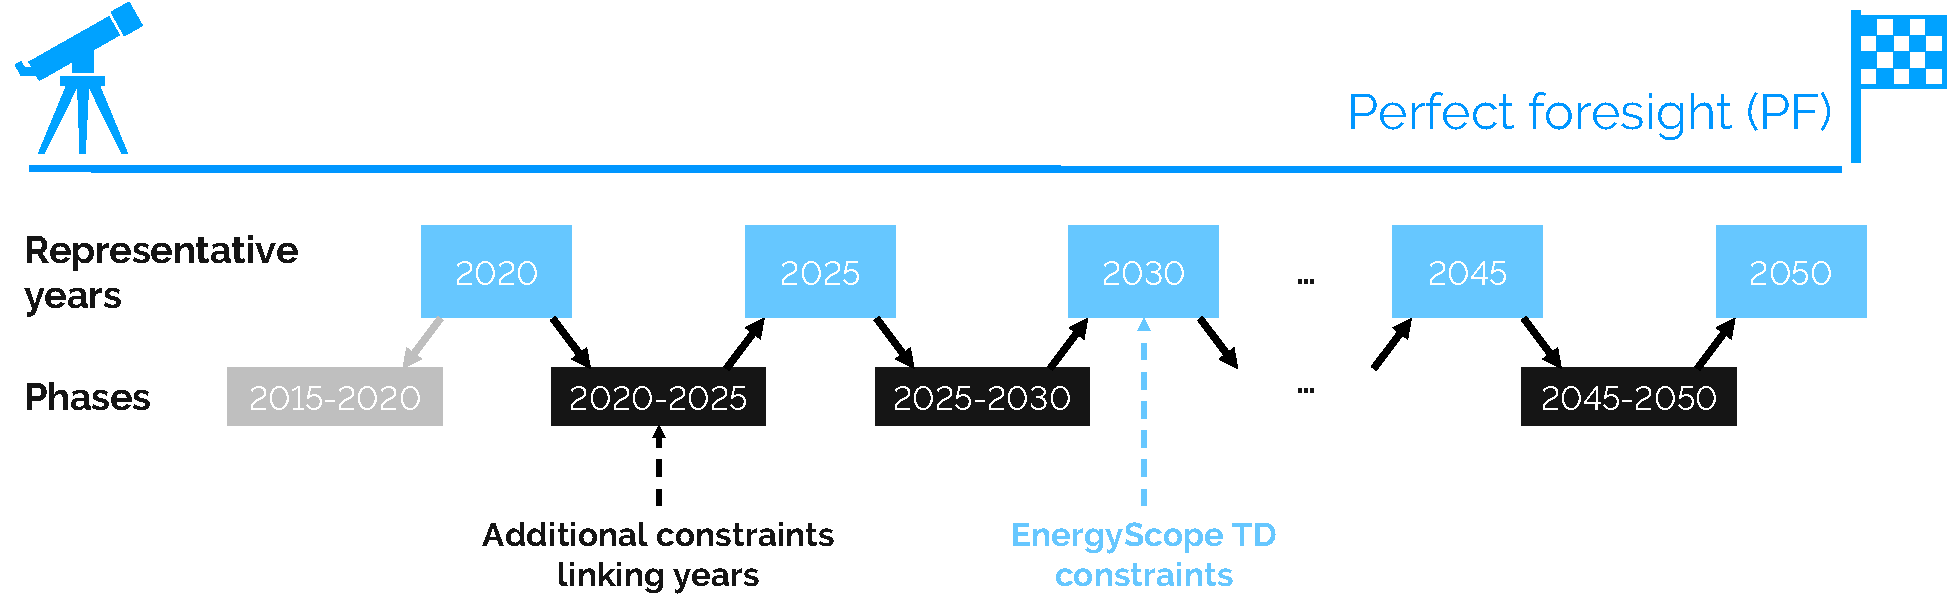
\includegraphics[width=\textwidth]{figures/ES_Pathway.pdf}
\caption{As one every five years paves the way from 2020 to 2050, the pathway methodology relies on 7 representative years (light blue boxes) where the model \acrfull{ESTD} is applied. Moreover, the formulation accounts for additional constraints (black boxes) linking years between each other. Finally, the initialisation of the pathway assumes that all capacities installed in 2020 have been built during the pseudo-phase 2015-2020 (grey box). The overall problem is the pathway model. Graph adapted from \cite{limpens2023pathway}.}
\label{fig:meth_path_methodology}
\end{figure}

\Cref{fig:meth_path_methodology} illustrates the methodology of EnergyScope Pathway\footnote{As represented in \Cref{fig:meth_path_methodology}, in the rest of the paper, the focus will only be put on the perfect foresight formulation where the entire transition is optimised in one optimisation, assuming a complete but uncertain knowledge of the different parameters until 2050. In the contrary, as studied in other works \cite{babrowski2014reducing,fais2016impact,heuberger2018impact}, the myopic approach consists of limiting the foresight and optimising the pathway via a sequence of shorter time windows, \eg 10 years, that might overlap each other. The impact of such a formulation for the model EnergyScope Pathway has also been extensively discussed by \citet{limpens2023pathway}.}. All the variables and constraints of the snapshot model (EnergyScope TD) are kept as is with an extra-dimension to relate them to a specific representative year, $y$. For instance, the energy balance is guaranteed at every hour of each of these years. The different yearly costs are computed similarly:

\begingroup
\belowdisplayskip=2pt
\abovedisplayskip=2pt
\begin{flalign} 
% Objective function + investment 
% adding 25pt space, otherwise flalign with two "&" would flush to the extreme left
\hspace{0pt} 
 \label{eq:c_inv}%3
 &\textbf{C\textsubscript{inv}}(y,j) = c_{\text{\emph{inv}}}(y,j) \textbf{F}(y,j) & \forall y \in \text{\emph{YEARS}}, \forall j \in \text{\emph{TECH}}\\
 \label{eq:c_maint}%4
 &\textbf{C\textsubscript{maint}}(y,j) = c_{\text{\emph{maint}}}(y,j) \textbf{F}(y,j) & \forall y \in \text{\emph{YEARS}}, \forall j \in \text{\emph{TECH}}\\ 
  \label{eq:c_op}%5
 &\textbf{C\textsubscript{op}}(y,i) = \sum_{\mathclap{t \in T }} c_{\text{\emph{op}}}(y,i) \textbf{F\textsubscript{t}}(y,i,t) t_{op} (t)  
 & \forall y \in \text{\emph{YEARS}}, \forall i \in \text{\emph{RES}}
 \end{flalign}
 \endgroup

\noindent where $\textbf{F}$ and $\textbf{F\textsubscript{t}}$ are the variables standing for the size of the installed capacities and the hourly consumption of the resources\footnote{When applied to technologies, $\textbf{F\textsubscript{t}}$ refers to their hourly power outputs.}. In terms of parameters, $c_{\text{\emph{inv}}}$, $c_{\text{\emph{maint}}}$ and $c_{\text{\emph{op}}}$ represent respectively the capex and the opex of the technologies and the cost of purchasing of the resources. For the sake of simplicity, the sum over the 8760 hours of the year is written as the sum over $t \in T $. 

Similarly, the computation of the emissions are also based on the \acrfull{GWP} of the resources:

\begingroup
\belowdisplayskip=2pt
\abovedisplayskip=2pt
\begin{flalign}
\hspace{0pt}
 \label{eq:GWP_tot}%8
 & \textbf{GWP\textsubscript{tot}}(y)  =    \sum_{\mathclap{i \in \text{\emph{RES}}}} \textbf{GWP\textsubscript{op}}(y,i) 
 & \forall y \in \text{\emph{YEARS}}\\
  \label{eq:GWP_op}%7
 & \textbf{GWP\textsubscript{op}}(y,i) = \sum_{\mathclap{t \in T }} gwp_{\text{\emph{op}}}(y,i) \textbf{F\textsubscript{t}}(y,i,t)  t_{op} (t) & \forall y \in \text{\emph{YEARS}}, \forall i \in \text{\emph{RES}}
\end{flalign}
\endgroup

\noindent
where $gwp_{\text{\emph{op}}}$ is the specific emissions (\ie in kt$_{\ce{CO2},\text{eq}}$/GWh) of each resource. Based on a \gls{LCA} approach and developed by the Intergovernmental Panel on Climate Change (IPCC) \cite{stocker2014climate}, this work considers the indicator ``GWP100a - IPCC2013'' to compute the emissions related to the use of resources. This includes the emissions due to the extraction, the transportation and the combustion of the energy carrier. Regarding the technologies, the collection of the ``grey'' \gls{GWP} linked to extraction of materials, the construction and end of life of each technology, $\mathit{gwp}_{\mathrm{constr}}$, is still a work in progress. Consequently, it is not included in this work and not accounted for.

Then, the main constraint to link years with each other is the one dictating the installed capacities at the end of each year:

\begingroup
\belowdisplayskip=2pt
\abovedisplayskip=2pt
\begin{flalign} 
\label{eq:F_newBuilt}%5
&\textbf{F}(y\textsubscript{stop},j) = \textbf{F}(y\textsubscript{start},j)
 + \textbf{F\textsubscript{new}}(p,j)
 - \textbf{F\textsubscript{old}}(p,j)
 - \sum_{\mathclap{p2 \in \text{\emph{PHASE}} \cup \{2015\_2020\}}} \textbf{F\textsubscript{decom}}(p,p2,j)& \notag \nonumber 
 \end{flalign}
\begin{flalign} 
 &&  \forall p \in \text{\emph{PHASE}}, \emph{y\textsubscript{stop}} \in \emph{Y\_STOP}(p), \emph{y\textsubscript{start}} \in \emph{Y\_START}(p), j \in \text{\emph{TECH}}
 \end{flalign}

\endgroup

\noindent
where $\textbf{F\textsubscript{new}}$, $\textbf{F\textsubscript{old}}$ and $\textbf{F\textsubscript{decom}}$ are the capacities respectively newly installed, having reached the end of their lifetime and prematurely decommissioned. Moreover, to account for the society inertia and to prevent unrealistically fast modal share change, constraints limit this change for the sectors of the low-temperature, the passenger mobility and freight mobility demands. The parameters $\Delta_{\mathrm{change,LT\_heat}}$, $\Delta_{\mathrm{change,pass}}$ and $\Delta_{\mathrm{change,freight}}$ respectively limit their respective modal share change up to 33\%, 50\% and 50\% per phase of 5 years.

Next, the total cost of the transition, $\textbf{C\textsubscript{tot,trans}}$, represents the objective function of EnergyScope Pathway model:

\begingroup
\belowdisplayskip=2pt
\abovedisplayskip=2pt
\begin{flalign} 
% Objective function + investment 
\label{eq:obj_func_v2}%1
% adding 25pt space, otherwise flalign with two "&" would flush to the extreme 
\hspace{0pt} \min \text{  } & \textbf{C\textsubscript{tot,trans}} = \textbf{C\textsubscript{tot,capex}} + \textbf{C\textsubscript{tot,opex}}&\\
\label{eq:Capex_v2}
& \textbf{C\textsubscript{tot,capex}} =
\sum_{\mathclap{p \in \text{\emph{PHASE}}\cup \{2015\_2020\}}} 
\textbf{C\textsubscript{inv,phase}}(p)
-
\sum_{\mathclap{j \in \emph{TECH}}} 
\textbf{C\textsubscript{inv,return}}(j)\\
  \label{eq:Copex_tot_v2}%5
& \textbf{C\textsubscript{tot,opex}} =  \textbf{C\textsubscript{opex}}(2020)
+ \emph{t\textsubscript{phase}}\cdot \tau\textsubscript{\emph{phase}}(p) \cdot \sum_{\mathclap{p \in \emph{PHASE}|y\textsubscript{start}\in \emph{P\_START}(p),y\textsubscript{stop}\in \emph{P\_STOP}(p)}} 
 \Big(\textbf{C\textsubscript{opex}}(y\textsubscript{start}) + \textbf{C\textsubscript{opex}}(y\textsubscript{stop}) \Big)/2&\\
\label{eq:path_annu_factor}
& \tau\textsubscript{\emph{phase}}(p) = 1/(1+\emph{i\textsubscript{rate}})^{\emph{diff\_2015\_year(p)}} &
%% GL_correction_v2 %% & \tau\textsubscript{\emph{phase}}(p) = 1/(1+\emph{i\textsubscript{rate}})^{\emph{diff\_2015\_year(p)}} &
\end{flalign}
\endgroup

\noindent
where $\emph{t\textsubscript{phase}}=5\,\text{years}$ and $\emph{diff\_2015\_year(p)}$ are respectively the duration of a phase between two representative years and the number of years between the middle of a phase and 2015 for a correct annualisation. The other variables in Eq. (\ref{eq:Capex_v2}-\ref{eq:Copex_tot_v2}) are detailed here below:

\begingroup
\belowdisplayskip=2pt
\abovedisplayskip=2pt
\begin{flalign} 
\label{eq:opex_yearly}
&\textbf{C\textsubscript{opex}} (y) = \sum_{\mathclap{j \in \emph{TECH}}} \textbf{C\textsubscript{maint}}(y,j) + \sum_{\mathclap{i \in \emph{RES}}} \textbf{C\textsubscript{op}}(y,i)&\forall y\in \emph{YEARS}\\
\label{eq:PhaseInv}%5
&\textbf{C\textsubscript{inv,phase}}(p) = \sum_{\mathclap{j \in \emph{TECH}}} \textbf{F\textsubscript{new}}(p,j)\cdot \tau\textsubscript{\emph{phase}}(p)\cdot \left(\emph{c\textsubscript{inv}}(\emph{y\textsubscript{start}},j) + \emph{c\textsubscript{inv}}(\emph{y\textsubscript{stop}},j)\right)/2&\notag\nonumber
\end{flalign}
\begin{flalign}
&&\forall p \in \emph{PHASE} | y\textsubscript{start}\in \emph{P\_START}(p),y\textsubscript{stop}\in \emph{P\_STOP}(p)
\end{flalign}
\endgroup

\noindent
and $\textbf{C\textsubscript{inv,return}}$ accounts for the residual value, also called \textit{salvage value}, of the technologies installed during the transition and having not reached the end of their lifetime by 2050. This last variable is crucial to avoid penalising heavy (and potentially long-lifetime) investments at the end of the transition as these assets would still be operational beyond 2050. The interested reader will find more information about its implementation and the formulation choices related to it in the work of \citet{limpens2023pathway}. Finally, the total emissions of the system over the transition is computed as an average sum over the different representative years of the emissions due to the consumption of the resources:

\begingroup
\belowdisplayskip=2pt
\abovedisplayskip=2pt
\begin{flalign} 
\label{eq:gwp_tot_transition}
&\textbf{GWP\textsubscript{tot,trans}}= \textbf{GWP\textsubscript{tot}}(2020) + \emph{t\textsubscript{phase}}\sum_{\mathclap{p \in \emph{PHASE}|y\textsubscript{start}\in \emph{Y\_START}(p),y\textsubscript{stop}\in \emph{Y\_STOP}(p)}}\left(\textbf{GWP\textsubscript{tot}}(y\textsubscript{start}) +\textbf{GWP\textsubscript{tot}}(y\textsubscript{stop}) \right)/2 &
\\
\label{eq:limit_gwp_trans}
& \textbf{GWP\textsubscript{tot,trans}} \leq \emph{gwp\textsubscript{lim,trans}}&
\end{flalign}
\endgroup

\subsection{Uncertainty quantification}
\label{subsec:meth:UQ}
In their systematic review, \citet{yue2018review} highlighted that a wide majority of studies addressing the optimisation of energy systems (\ie 75\% out of the 134 reviewed studies) were not investigating the impact of uncertainties. However, disregarding these impacts can have drastic consequences on the system design. For instance, historical low \gls{NG} prices have led to overcapacity of gas \gls{CCGT} in Europe \cite{moret2020overcapacity} and even the prematurely decommissioning of a brand new 1.3~GW \gls{CCGT} in the Netherlands \cite{CCGT_NDLS}. This is why accounting for uncertainty is \gls{ESOMs} is crucial \cite{mavromatidis2018uncertainty}, especially when it comes to optimise several decades in the inherently uncertain future \cite{peace2008insights}.

This section aims then at briefly presenting the method followed to first characterise these uncertainties, then to quantify their impact on the objective function (\ie the total transition cost) as well as other outputs of interest (\eg amount of molecules imported from abroad) and finally, the screening and selection of the parameters to analyse.

\subsubsection{Uncertainty characterisation and sampling}
\label{subsubsec:UQ:UC}
Before quantifying the impact of the uncertainty of the parameters, it is of paramount importance to characterise these as accurately as possible, ideally with their respective probability density functions (PDFs) to carry out stochastic analysis \cite{dantzig1955linear}, for instance. However, such data are often seldom \cite{marnay2006addressing} and workarounds are therefore needed to cope with this challenge. Among others, this work uses the method developed by \citet{Moret2017} that defines relative ranges of variation for different groups of parameters. Originally defined for the Swiss case and the target future year of 2035 (\ie 20 years after the date of the analysis, N=20 in \cite{Moret2017}), these ranges have been adapted for the Belgian energy system and recomputed to align with the 5-year phase between each representative year of the transition. Moreover, some ranges have been added to account for new parameters coming from the pathway formulation described in \Cref{subsec:meth:ES_Pathway} like the society inertia.

\Cref{tab:UC_short} gives the uncertainty ranges of some key parameters. Like other works \cite{li2019renewables,coppitters2021robust}, the uncertain parameters are assumed to be independent and uniformly distributed between their respective lower and upper bounds. A particular attention is to pay to the potential installation of \gls{nuke-SMR}, at the bottom of \Cref{tab:UC_short}. As detailed in \Cref{sec:case_study}, the availability of such a technology is uncertain but would not be before 2040. Consequently, for \gls{nuke-SMR}, the parameter $f_{\mathrm{max,nuclear\,SMR}}$ influences the maximum capacity (\ie 6~GW) to install to translate somehow the readiness of this technology. If it is (i) smaller than 0.6, there is no possibility to install nuke-SMR during the transition; (ii) between 0.6 and 0.8, these 6~GW can be installed only in 2050; (iii) between 0.8 and 0.9, these can be installed from 2045 onward and; (iv) higher than 0.9, the prescribed maximum capacity can be installed from 2040 onward. Based on the local sensitivity analysis carried out by \citet{PATHS2050}, the current work also considers a [-40\%; +44\%] range on the capex of SMR, on top of the uncertainty about the availability. Finally, the the cost of purchasing of renewable electrofuels presents a wide range, [-64.3\%; +179.8\%], like the other imported commodities.

The exhaustive list of the parameters accounted in this work is presented in \Cref{app:UC_full}.

\begin{table}[htbp]
\caption{Illustration of the uncertainty characterisation for different parameters for the year 2025. $^{(a)}$ Per \cite{Moret2017PhDThesis}, \og I: investment-type, II: operation-type (constant uncertainty over time), III: operation-type (uncertainty increasing over time)\fg. $^{(b)}$ The nominal values of each of the parameters is 0, meaning no variation compared to the nominal values of the impacted parameter in the model. $^{(c)}$ This range has been inferred from the local sensitivity analysis performed by \citet{PATHS2050}. Abbreviations: \acrfull{EUD}, \acrfull{FC}, \acrfull{PV}.}
\label{tab:UC_short}
\centering
\resizebox{\textwidth}{!}{
\begin{tabular}{l l l c c c}
\toprule
\multirow{2}{*}{\textbf{Category}} & \multirow{2}{*}{\textbf{Parameter}} & \multirow{2}{*}{\textbf{Meaning}} & \multirow{2}{*}{\textbf{Type}$^{(a)}$}  & \multicolumn{2}{c}{\textbf{Relative variation$^{(b)}$}}\\
    & & & &	 min 	&	 max \\ 	
\midrule		
\multirow{2}{*}{\textbf{Cost of purchasing}} & $c_{\mathrm{op,fossil}}$ & Purchase fossil fuels & II & -64.3\% & 179.8\% \\
& $\bm{c_{\mathrm{op,electrofuels}}}$ & \textbf{Purchase electrofuels} & \textbf{II} & \textbf{-64.3\%} & \textbf{179.8\%} \\
\midrule
\multirow{5}{*}{\textbf{Investment cost}} &$c_{\mathrm{inv,car}}$ & Capex car  & I & -21.6\% & 25.0\% \\
& $c_{\mathrm{inv,e\_prop}}$ & Capex electric motor & I & -39.6\% & 39.6\% \\
& $c_{\mathrm{inv,fc\_prop}}$ & Capex fuel cell engine & I & -39.6\% & 39.6\% \\
& $c_{\mathrm{inv,PV}}$ & Capex PV & I & -39.6\% & 39.6\% \\
& $\bm{c_{\mathrm{inv,nuclear\_SMR}}}$ & \textbf{Capex nuclear SMR}$^{(c)}$ & \textbf{I} & \textbf{-40.0\%} & \textbf{44.0\%} \\
\midrule
\multirow{1}{*}{\textbf{Efficiency}} &$\eta_{\mathrm{e\_prop}}$ & Efficiency electric motor & I & -28.7\% & 28.7\% \\
\midrule
\multirow{2}{*}{\textbf{Potential installed capacity}} &$f_{\mathrm{max,PV}}$ & Max capacity PV & I & -24.1\% & 24.1\% \\
& $f_{\mathrm{max,windon}}$ & Max capacity onshore wind & I & -24.1\% & 24.1\% \\
\midrule
\multirow{2}{*}{\textbf{Hourly load factor}} & $c_{\mathrm{p,t,PV}}$ & Hourly load factor PV & II & -22.1\% & 22.1\% \\
& $c_{\mathrm{p,t,winds}}$ & Hourly load factor wind turbines & II & -22.1\% & 22.1\% \\
\midrule
\multirow{2}{*}{\textbf{Resource availability}} & $avail_{\mathrm{elec}}$ & Available electricity import & I & -32.1\% & 32.1\% \\
& $avail_{\mathrm{biomass}}$ & Available local biomass & I & -32.1\% & 32.1\% \\
\midrule

\multirow{2}{*}{\textbf{End-use demand}} & $pass\_EUD$ & Passenger mobility EUD & III & -7.5\% & 7.5\% \\
& $industry\_EUD$ & Industry EUD & III & -20.5\% & 16.0\% \\
\midrule

\multirow{4}{*}{\textbf{Miscellaneous}} &$i_{\mathrm{rate}}$  & Interest rate & I & -46.2\% & 46.2\% \\
& $\Delta_{\mathrm{change,freight}}$ & Modal share change freight mobility & - & -30\% & 30\% \\
& $\Delta_{\mathrm{change,pass}}$ & Modal share change passenger mobility & - & -30\% & 30\% \\
& $\bm{f_{\mathrm{max,nuclear\,SMR}}}$ & \textbf{Potential capacity nuclear SMR} & \textbf{-} & \textbf{0} & \textbf{1} \\

\bottomrule							

\end{tabular}}
\end{table}

Following the methodology defined by \citet{Moret2017}, uncertainties of types I and II keep the same range for the whole transition. However, parameters with an uncertainty increasing over time, type III, (\ie end-use demands, in this case) will have a wider and wider range over the transition. In this work, a +50\% linear increase has been arbitrarily set between the width of the range of such parameters in 2025 and the same ranges in 2050. In \Cref{fig:ranges_transition}, this means that for type III uncertainties only, $R_{2050}^+$ is 50\% bigger than $R_{2025}^+$ and $R_{2050}^-$ is 50\% smaller than $R_{2025}^-$. For uncertainties of types I and II, the relative variation versus the nominal value remain the same over the transition. Inspired by \citet{guevara2022modeling}, this figure also shows how the values of one parameter are set over the transition for each generated sample: starting from the nominal value in 2020, values of the uncertain parameter do not zigzag from 2025 to 2050 (\ie similar to $\alpha=0$ in \cite{guevara2022modeling}). For instance, if one parameter is sampled at its upper bound, it will stick to this upper band for all the representative years of the transition.

\begin{figure}[!htbp]
\centering
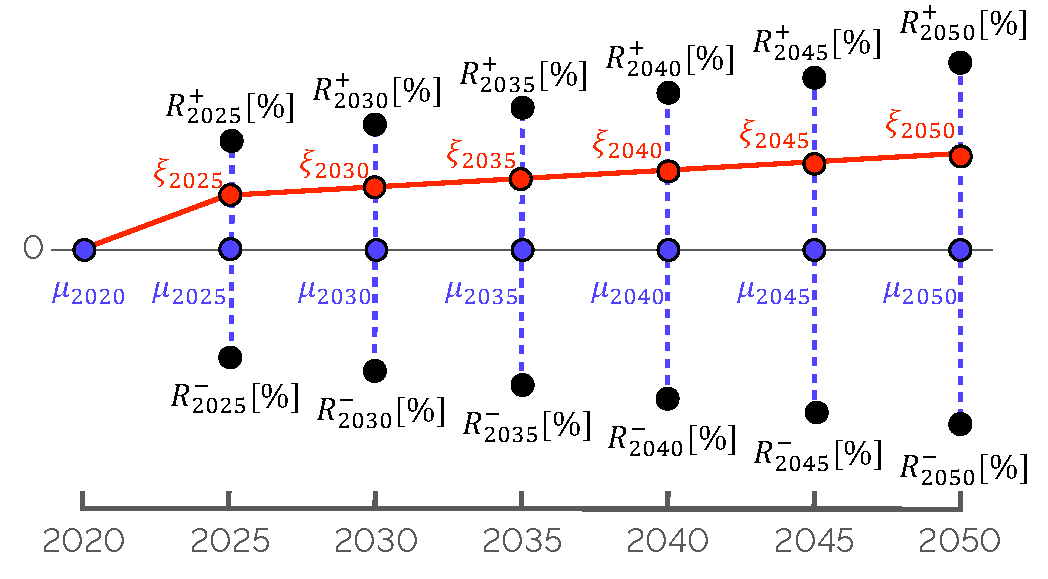
\includegraphics[width=0.5\textwidth]{figures/ranges_transition.pdf}
\caption{$\mu_{2020}$, $\mu_{2025}$, ...,  $\mu_{2050}$ are the nominal values equal to 0 as the uncertain parameters represent a relative increase/decrease of actual parameters of the model. $R^+$ and $R^-$ are respectively the upper and lower bounds of the range and $\xi_{2025}$, $\xi_{2030}$, ...,  $\xi_{2050}$ are the values taken by one parameter for a specific sample for each of the representative years of the transition, always starting from the nominal value in 2020. The graph has been adapted from \cite{guevara2022modeling}.}
\label{fig:ranges_transition}
\end{figure}

\subsubsection{Polynomial Chaos Expansion}
\label{subsubsec:UQ:PCE}

We used \gls{PCE}, an approach for surrogate-assisted \gls{UQ}, to propagate uncertainties in input parameters through the system model. This allowed us to assess statistical moments on the quantity of interest and determine Sobol' indices~\cite{coppitters2020robust}. To construct a PCE of the EnergyScope Pathway model, we employed the open-source Python framework RHEIA~\cite{coppitters2022rheia}, which was developed within our research group.\par

The PCE model ($\hat{M}$) is a representation of the relationship between the input parameters and the output variable of interest in the EnergyScope Pathway model ($M$). This representation is constructed as a truncated series of multivariate orthonormal polynomials $\bm{\Psi}$, weighted by coefficients $u$:

\begin{equation}
\hat{M} \left( \bm{\xi} \right) = \sum_{\bm{\alpha} \in \mathcal{A}^{d,p}} u_{\bm{\alpha}} \bm{\Psi}_{\bm{\alpha}} \left( \bm{\xi} \right) \approx M \left( \bm{\xi} \right), 
\end{equation}

where the vector $\bm{\xi} = (\xi_1,\xi_2, \dots \xi_d)$ comprises the independent random input parameters (\autoref{app:UC_full}), $d$ corresponds to the number of input distributions and $\bm{\alpha}$ is a multi-index. As uniform distributions are considered, the Legendre polynomials are adopted, as they are the associated family of polynomials that are orthogonal with respect to standard uniform distributions~\cite{Sudret2014}.\par 

A truncation scheme is implemented to restrict the number of multivariate polynomials in the series. This is done based on two factors: a specified limiting polynomial order ($p$) and the number of uncertain parameters ($d$) involved. The multivariate polynomial order $|\bm{\alpha}|$ is the summation of the orders for each univariate polynomial in the multivariate polynomials. Thus, only the multi-indices corresponding to an order that is less than or equal to the specified limiting order are retained and stored in the truncated series denoted as $\mathcal{A}^{d,p}$:

\begin{equation}
\mathcal{A}^{d,p} = \left \{ \bm{\alpha} \in \mathbb{N}^d : |\bm{\alpha}| \leq p \right \}. 
\end{equation}

The number of multi-indices satisfying this condition is as follows:
\begin{equation}
\mathrm{card} \left( \mathcal{A}^{d,p} \right) = {p + d \choose p} = \dfrac{\left( d + p \right) !}{d! p!} = P + 1.
\label{eq:pce:nterms}
\end{equation}

The coefficients ($u_0, u_1, \dots, u_{P+1}$) are quantified using a regression method applied to orthonormal polynomials~\cite{Sudret2014}. To ensure a well-posed least-square minimisation, it is recommended to have a number of training samples at least twice the number of coefficients~\cite{Sudret2014}. Therefore, $2 \left( P+1 \right)$ samples are evaluated in the system model, and the model response for each quantity of interest is recorded. To generate the training samples, the quasi-random Sobol' sampling technique is employed~\cite{bratley2003implementing}. As a low-discrepancy sequence, this technique exhibits the main advantage to investigate efficiently and (almost) uniformly the hypercube of uncertainties, unlike uniformly distributed random numbers.\par

The process of defining the polynomial degree includes incrementally increasing it until a desired level of accuracy is achieved~\cite{coppitters2022rheia}. Starting with $p=1$, a PCE is constructed and the \gls{LOO} error is evaluated. If the \gls{LOO} error is below a specified threshold, the corresponding polynomial order is considered sufficient for generating an accurate PCE. However, if the error exceeds the threshold, the order is increased, and additional samples are generated using Eq.~\ref{eq:pce:nterms}.

For the specific study of this work, a polynomial order of 2 is necessary (with 1260 training samples as per Eq.~\ref{eq:pce:nterms}) to achieve a \gls{LOO} error below \SI{1}{\%} for the total transition cost.\par

Lastly, the statistical moments can be analytically derived from the PCE coefficients, eliminating the need for further model evaluations. To clarify, the mean $\mu$ and standard deviation $\sigma$ are obtained as follows:
\begin{align}
\mu &= u_0,\\
\sigma^2 &= \sum_{i \neq 0 } u_{i}^2 .
\label{eq:pce:statmom}
\end{align}

Furthermore, the Sobol' indices can also be determined analytically. The total-order Sobol' indices ($S_i^{T}$) assess the overall influence of a stochastic input parameter on the performance indicator, encompassing all possible interactions:

\begin{equation}
S_i^{T} = \sum_{\bm{\alpha} \in A_i^T}^{} u_{\bm{\alpha}}^2/\sum_{i=1}^P u_i^2 ~~~~~~ A_i^T = \{\bm{\alpha} \in A | \alpha_i > 0\}.
\end{equation}

Here, $A$ denotes the collection of all PCE coefficients, and $\alpha_i$ corresponds to the coefficient associated with the uncertain parameter $i$.\par

\subsubsection{Preliminary grouping, screening and selection}
\label{subsubsec:UQ:screening}
The model accounts for thousands of parameters. The computational burden to consider all of them separately would be completely overwhelming ($\sim 10^7$ model runs). Therefore, similarly to other works \cite{Moret2017,limpens2020impact}, the parameters have been grouped to affect similar parameters. For instance, the uncertainty on the cost of purchasing of renewable electrofuels, $c_{\mathrm{op,electrofuels}}$, identically affects the cost of e-hydrogen, e-methane, e-ammonia and e-methanol. Indeed, besides their respective specificities, each of these fuels will be similarly affected by the variation of cost of electricity or the electrolyser, that drive the majority of their cost of purchasing \cite{h2coalition}. Similarly, the uncertainties impacting the industrial demand, $industry\_EUD$, alters equally the industrial high- and low-temperature and electricity demands as well as the non-energy demand.

After this phase of grouping, a preliminary screening was necessary to identify the key parameters to account for in this \gls{GSA}. \citet{rixhon2021role} performed a similar sensitivity analysis on the 2050 Belgian whole-energy system under different \ce{CO2}-limits using a snapshot model (\ie EnergyScope TD \cite{limpens2019energyscope}). Screening the results of this work, we have selected a subset of parameters and added others that were intrinsic to the pathway formulation, \eg modal share changes, or related to the integration of nuclear SMR, $f_{\mathrm{max,nuclear\,SMR}}$. The exhaustive list of these 34 parameters is presented in Appendix \ref{app:UC_full}.

%%%%%%%%%%%%%%%%%%%%%%%%%%%%%%%%%%%%%%%%%%%%%%%%%%%%%%%%%%%%%%%%%%%%%%%%%%%%%%%%%%%%%%%%%%%%%%%%%%%%%%%%%%%%%%%%%%%%%%%%%%%%%           CASE STUDY %%%%%%%%%%%%%%%%%%%%%%%%%%%%%%%%
%%%%%%%%%%%%%%%%%%%%%%%%%%%%%%%%%%%%%%%%%%%%%%%%%%%%%%%%%%%%%%%%%%%%%%%%%%%%%%%%%%%%%%%%%%%%%%

\section{Case study: the Belgian whole-energy system}
\label{sec:case_study}
As detailed by \citet{limpens2023pathway}, the analysis carried out in this work can be applied to any regional whole-energy system. As a densely-populated and highly-industrialised country with limited local renewable potentials (\ie mainly solar and wind), the transition of Belgium from a fossil-dominated system in 2020 (see Appendix \ref{sec:app:bel_2020}) to carbon-neutrality in 2050 makes it an intricate case study. Moreover, this case study and the subsequent analyses can be transferred - to some extent - to other industrialised countries highly dependent on fossil fuels with limited local renewable potentials (\eg the Netherlands or Germany) \cite{dommisse2020modelling}. This section presents the different demands to satisfy as well as the resources available and the conversion technologies to supply those. The focus here is given to the renewable molecules to import from abroad as well as the techno-economic details of nuclear SMR. For a comprehensive understanding and detailed descriptions of the technologies, please refer to the documentation \cite{readthedocs_pathway}. Finally, the \ce{CO2}-budget to spend over the 2020-2050 transition is presented.


\subsection{Demands}
\label{subsec:cs:demand}

End-use demands, exogenously imposed as inputs to the model, are characterised by yearly quantities to satisfy and are also spread over the different hours of each representative years of the transition, in order to account for their daily or seasonal variability. In this work, the yearly \gls{EUD} for all sectors are calculated from the rather slightly increasing forecast carried out by the European Commission for Belgium (see Appendix 2 in report \cite{EuropeanCommission2021}). Although, given a significant and unsubstantiated discrepancy in the non-energy use forecasts compared to their previous report (\ie +80\% over the 2020-2030 time window), the evolution trend of the \gls{NED} of the current work has been inferred from this previous edition, published in 2016, \cite{EuropeanCommission2016}. Looking at \Cref{fig:cs_demands}, between 2020 and 2050, one observes a noteworthy increase of the electricity (+40\%), passenger (+45\%) and freight mobility (+35\%) demands. The rise of the non-energy demand is more limited, \ie +6\%, whereas the heating demands is forecast to decrease: -11\% and -3\% respectively for the low and high-temperature heat demands. Regarding the center graph of \Cref{fig:cs_demands}, it is nothing more than the aggregation of the same data as the left graph but per category, rather than per sector, with the non-energy demand being associated with the industry. This illustrates how industrialised is Belgium, compared to households and services, and, consequently, highly energy intensive.
As far as the hourly discretisation of these demands is concerned, time series are based on historical values of 2015 for parts of electricity and low-temperature heating demands \cite{Limpens2020}. A daily time series is used for the passenger mobility and applied similarly to every typical days. Finally, for the other demands, the yearly demand is distributed uniformly over the different hours of the year.

\begin{figure}[!htbp]
\centering

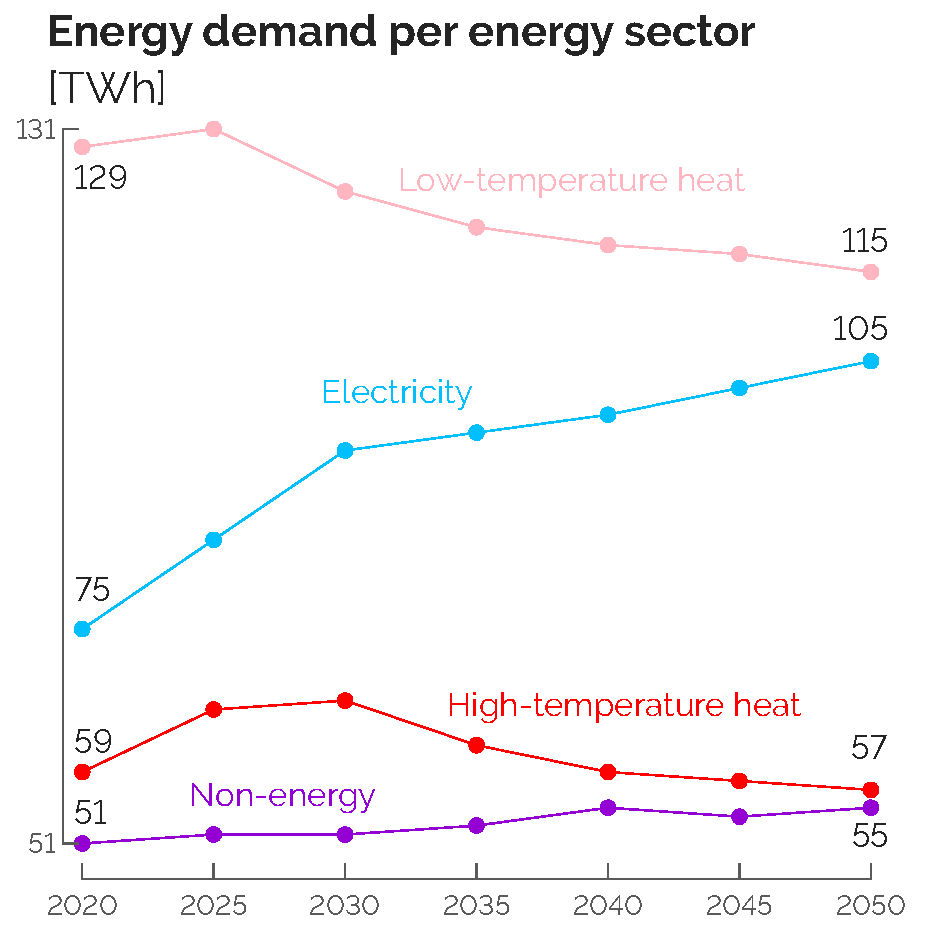
\includegraphics[width=0.32\textwidth]{figures/EUD_sec.pdf}
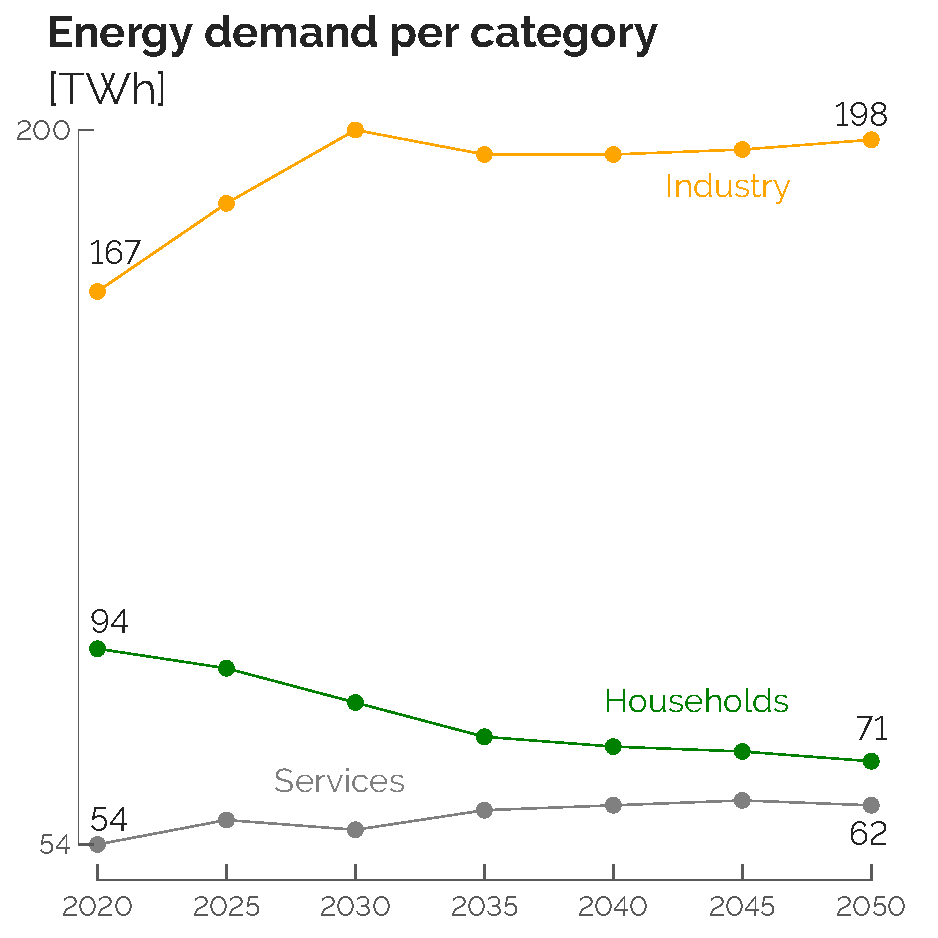
\includegraphics[width=0.32\textwidth]{figures/EUD_cat.pdf}
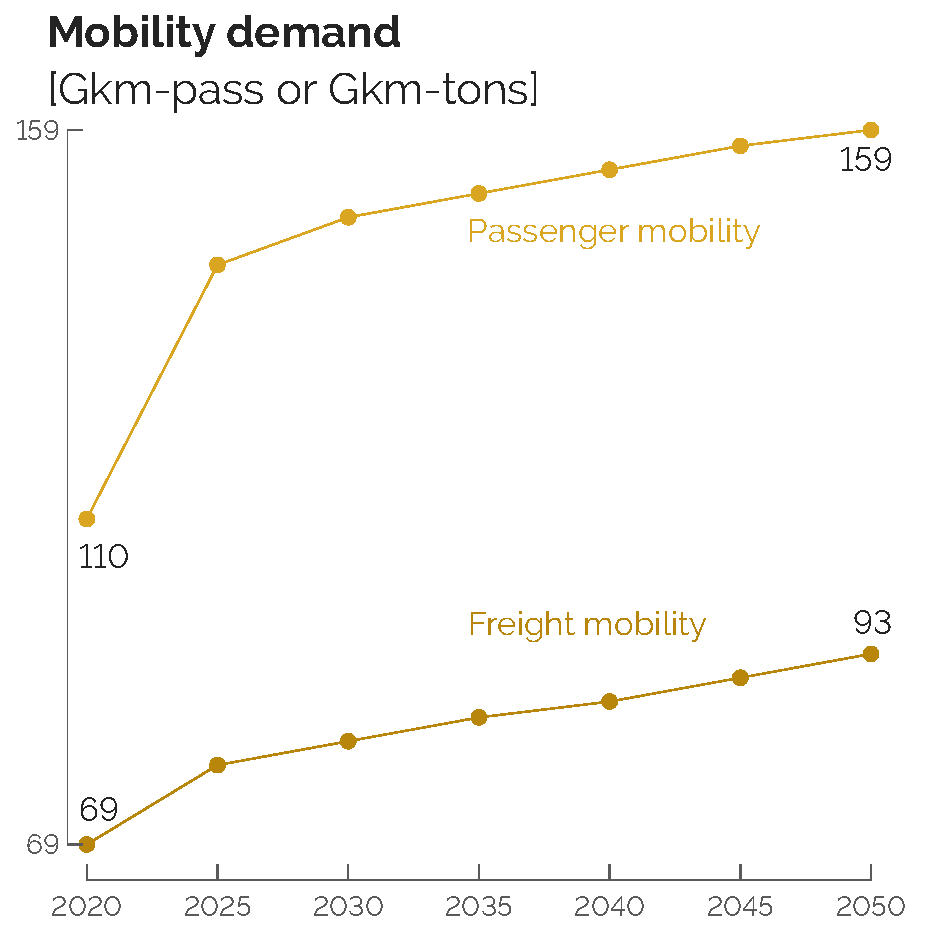
\includegraphics[width=0.32\textwidth]{figures/EUD_mob.pdf}
\caption{EnergyScope splits the whole-energy system \acrfull{EUD} in two sets: the ones that can be expressed in terms of energy (TWh) and the others regarding the mobility, expressed in distance (kilometers). This figure presents the nominal values of each of these demands. The only difference between the left and center graphs is the aggregation of the same data either per sector or per category. In the center graph, the non-energy demand has been associated with the industrial demand. As detailed by \citet{rixhon2022integration}, the non-energy demand is expressed in tons of physical products (\ie \acrfull{HVC}, ammonia and methanol) and then translated into their respective energy equivalent, in TWh. The sharp rise of the two mobility demands most probably come from the assumption to come back the original trends after the COVID crisis. Graphs have been adapted from \cite{limpens2023pathway}.}
\label{fig:cs_demands}
\end{figure}

\subsection{Resources}
\label{subsec:cs:resources}
To supply the aforementioned demands, EnergyScope Pathway implements a variety of resources defined by their cost of purchasing, $\mathit{c}_{\mathrm{op}}$, their global warming potential, $\mathit{gwp}_{\mathrm{op}}$, as well as their 
availability, as detailed by \citet{limpens2023pathway}. Besides the evolution of their respective cost (see \Cref{fig:cs_resources_cost}), the resources are either limited or unlimited in terms of availability and either renewable or not. The limitation in terms of availability can be direct or indirect. On one hand, woody (23.4\,TWh) and wet biomass (38.9\,TWh) are limited by their local potentials and the consumption of waste (17.8\,TWh) and coal (33.4\,TWh) is assumed not to exceed the current use. On the other hand, wind, solar, hydro and uranium are limited by the technical potentials respectively, of \gls{PV} panels (59.2\,GW), onshore (10\,GW) and offshore (6\,GW) wind turbines, run-of-the-river power plants (0.1\,GW) and nuclear power plants (6\,GW). Imported electricity is limited in two ways: the potential of instantaneous capacity of interconnection with neighbouring countries (\ie 11.9\,GW by 2050 \cite{ELIA_2050}) and a limitation to 30\% of the yearly electricity end-use demand (\ie 32.4\,TWh by 2050). Then, looking at the renewability of a resource, an energy carrier is assumed to be renewable (\ie $\mathit{gwp}_{\mathrm{op}}=0$\,kt$_{\ce{CO2},\text{eq}}$/GWh) when it is produced from renewable energy sources \cite{eu2003directive} that are \textit{non-fossil sources naturally replenished on a human timescale (\ie wind, solar, geothermal, wave, tidal, hydro-power, biomass)} \cite{ellabban2014}. In the current work, the electrofuels (\ie e-methane, e-hydrogen, e-methanol and e-ammonia) are assumed to be ``sustainable" in the sense that they do not increase the concentration of \ce{CO2} in the atmosphere \cite{rixhon2021terminology}. Regarding specifically at these electrofuels, \citet{h2coalition} has carried out an extensive techno-economic analysis to assess their respective cost of purchasing, identifying some key locations from which exporting these energy carriers (\eg Chile, Australia or Morocco). As the amount to import from each of these locations is hard to forecast, the current work considers average cost between the different locations. Besides these, every other resources have their specific \gls{GWP} like coal ($\mathit{gwp}_{\mathrm{op,coal}}=0.40$\,kt$_{\ce{CO2},\text{eq}}$/GWh), natural gas ($\mathit{gwp}_{\mathrm{op,NG}}=0.27$\,kt$_{\ce{CO2},\text{eq}}$/GWh) or the fossil-based molecules equivalent to the electrofuels (\eg $\mathit{gwp}_{\mathrm{op,ammonia}}=0.46$\,kt$_{\ce{CO2},\text{eq}}$/GWh or $\mathit{gwp}_{\mathrm{op,methanol}}=0.41$\,kt$_{\ce{CO2},\text{eq}}$/GWh).



\begin{figure}[!htbp]
\centering

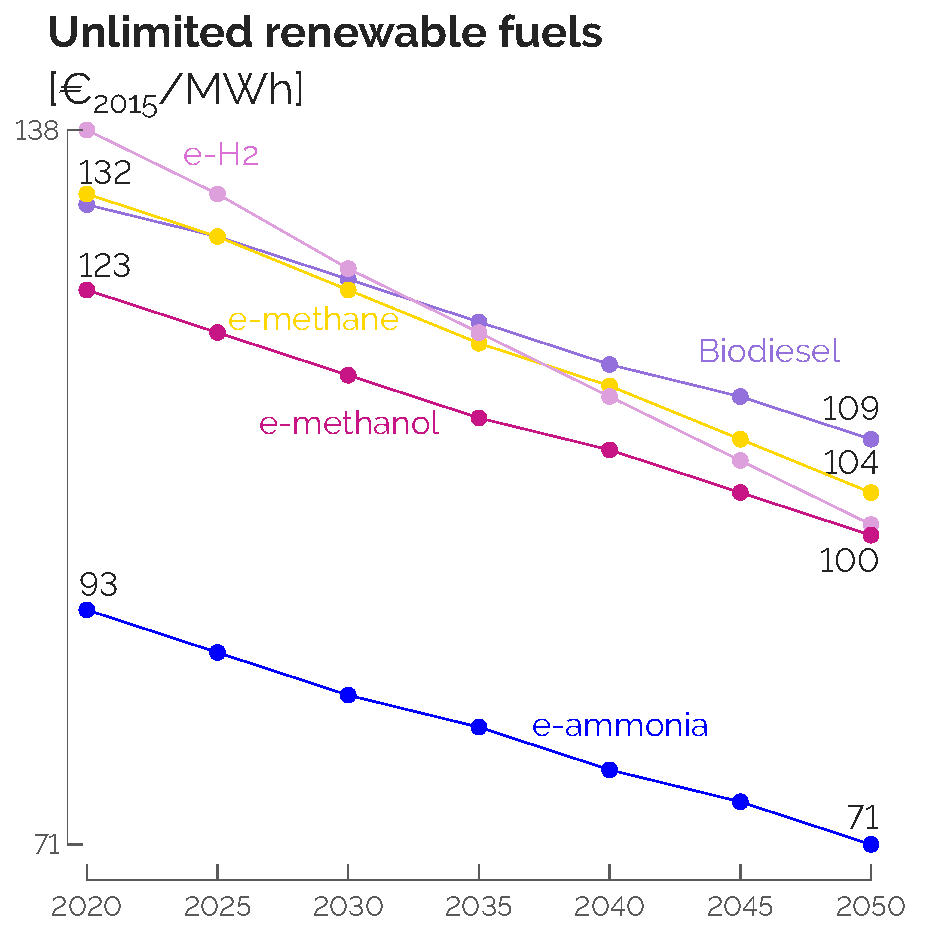
\includegraphics[width=0.32\textwidth]{figures/Res_ren.pdf}
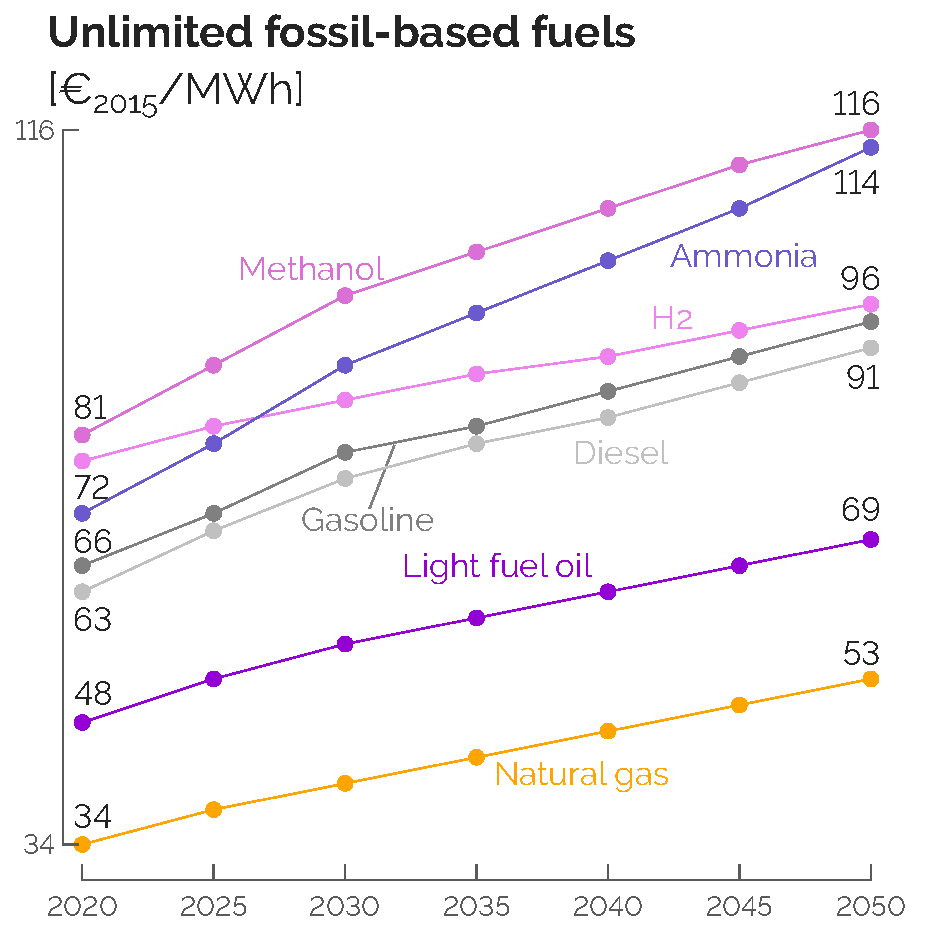
\includegraphics[width=0.32\textwidth]{figures/Res_foss.pdf}
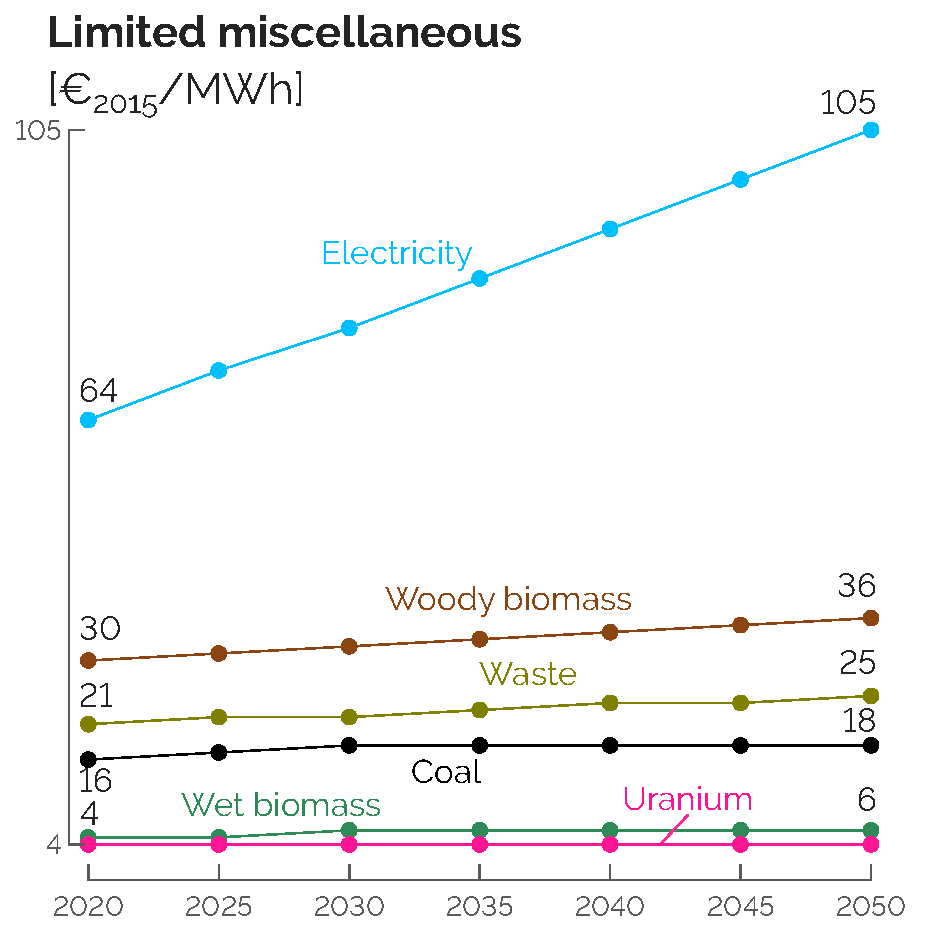
\includegraphics[width=0.32\textwidth]{figures/Res_misc.pdf}
\caption{Cost of purchasing of the different resources. Besides the free local renewables (\ie sun, wind and hydro) limited by technical potentials, EnergyScope accounts for renewable energy carriers and their respective fossil counterparts (left and center graphs). These fuels can be imported from abroad without limitation on their availability. On the other hand, other carriers are limited either by their local potentials (\ie biomass and waste) or other considerations like the power grid interconnections or the capacity of nuclear power plants respectively for the electricity and the uranium.}
\label{fig:cs_resources_cost}
\end{figure}


\subsection{Nuclear SMR and other conversion technologies}
\label{subsec:cs:technologies}
Finally, as the end-use demands are defined as energy (and non-energy with the \gls{NED}) services rather than a certain volume of oil or solar irradiance, technologies are implemented to convert these resources into the end-use demands. Each technology is defined by a CAPEX ($c_{\text{\emph{inv}}}$) that is annualised, an annual OPEX ($c_{\text{\emph{maint}}}$) and a lifetime. Production and conversion technologies (\ie \gls{CCGT}, car or boiler) have a conversion efficiency where storage technologies (\ie thermal storage, battery or molecule storage) exhibit their own charge/discharge losses. Eventually, there are also infrastructure technologies like the grid or the \gls{DHN} that allow to account for the investment necessary, respectively, to integrate more intermittent renewables in the power sector and the expand the use of centralised heating systems.

A specific attention is to put on the implementation of nuclear small modular reactors whereas the 6\,GW of conventional nuclear are assumed to drop to 2\,GW in 2025 and total phase-out by 2035. Similarly to the analysis of \citet{PATHS2050} and in line with the Belgian Nuclear Research Centre (SCK-CEN) \cite{SCK-CEN_SMR}, nuclear SMR is implemented with the features listed in \Cref{tab:SMR_features}. Where most of the features are similar to conventional nuclear power plants, it differs from these on two main points: their potential year start, 2040, and their flexibility. Indeed, unlike the current nuclear power plants, constrained in the model to produce a constant power output at every hour of the year, SMRs, as the name suggests, are modular in the sense that their production is flexible between 0 and their full capacity independently at each hour.


\begin{table}[htbp]
\caption{Nominal features of the nuclear small modular reactors (SMR) in EnergyScope. SMR exhibits the advantage to have a fully flexible production (\ie between 0 to the full capacity) unlike conventional nuclear that is constrained to produce a constant baseload at every hour of the year. $^{(a)}$ As SMRs are foreseen, if installed, to be around the same locations (\ie Thiange and Doel) as the conventional nuclear power plants and using the same area in kW/ha, the same 6\,GW are assumed to be the maximum capacity for SMRs. $^{(b)}$ This annual availability accounts for yearly maintenance where the reactors might not operate or, at least, not at their maximum capacity. $^{(c)}$ 2040 is the soonest year at which \gls{nuke-SMR} could be available. It is a very ambitious and optimistic objective as SCK-CEN announces a demonstrator operational by 2035-2040.}
\label{tab:SMR_features}
\centering
\begin{tabular}{l c c|c}
\toprule
\multirow{2}{*}{\textbf{Feature}} & \multirow{2}{*}{\textbf{Value}} & \multirow{2}{*}{\textbf{Unit}} & \textbf{Similarity with}\\
 & & & \textbf{conventional nuclear}\\
\midrule
Capex & 4850 & €/kW & \checkmark\\
Annual Opex & 103 & €/kW/year & \checkmark\\
Lifetime & 60 & year & \checkmark\\
Efficiency & 40\% & -& \checkmark\\
Maximum capacity & 6$^{(a)}$ & GW & \checkmark\\
Annual availability & 85\%$^{(b)}$ & -& \checkmark\\
\midrule
Operational year & 2040$^{(c)}$ & - & \xmark\\
Flexibility & Full & - & \xmark\\
\bottomrule							

\end{tabular}
\end{table}

\subsection{Transition \ce{CO2}-budget}
\label{subsec:cs:CO2-budget}
In most of the studies carried out on the pathway optimisation of a whole-energy system, a \ce{CO2}-trajectory is \textit{a priori} set to reach carbon-neutrality by 2050. \citet{nerini2017myopic} used the emission trajectory indicated by the UK's Committee on Climate Change in their analysis of the impact of limited foresight to achieve the target of 80\% reduction of \gls{GHG} by 2050 in the United Kingdom. In their assessment of the impacts of economy-wide emissions policies in the water-energy-land nexus, \citet{licandeo2023assessing} analysed different \ce{CO2}-trajectories considering more or less severely water scarcity for the US. \citet{poncelet2016myopic} with LUSYM (Leuven University SYstem Model) and \citet{PATHS2050} with TIMES-BE also set decreasing emission trajectories in their analysis of respectively the Belgian power sector and whole-energy system.  Others only set the objective as the carbon-neutrality by 2050. For instance, \citet{heuberger2018impact} investigated the impact of different factors (\eg limit of the foresight in the future, availability of ``unicorn technologies'' or committed versus market-driven decarbonisation strategies) to reach this ultimate objective in the UK system.

In this work, the authors have decided to take a different approach since the effect of greenhouse gases is cumulative over time. Indeed, the \ce{CO2}, as well as the other greenhouse gases, emitted today will remain in atmosphere for a long time and keep on contributing to the global warming. Consequently, the current analysis does not set a limit of emissions for every of the representative years but rather on the overall emissions over the transition. In other words, starting from the annual 123\,Mt$_{\ce{CO2},\text{eq}}$ in 2020, an budget has been arbitrarily attributed to the Belgian whole-energy system until 2050. This budget, 1.2\,Gt$_{\ce{CO2},\text{eq}}$, has been computed using a rule of three between the emissions of Belgium in 2020, these of the world (\ie 34.8\,Gt$_{\ce{CO2},\text{eq}}$ \cite{ourworldindata_CO2_world} and the global budget to have a decent chance (medium confidence) of limiting warming to 1.5°C of 420\,Gt$_{\ce{CO2},\text{eq}}$ \cite{IPCC_CO2_budget}. Therefore, in this work, a limit has been put on $\emph{gwp\textsubscript{lim,trans}}=1.2\,\text{Gt}_{\ce{CO2},\text{eq}}$ in
Eq.\,(\ref{eq:limit_gwp_trans}). This is another sign of the urgency to act to mitigate climate change as this 30-year budget represents only 10 years of the current emissions.

%%%%%%%%%%%%%%%%%%%%%%%%%%%%%%%%%%%%%%%%%%%%%%%%%%%%%%%%%%%%%%%%%%%%%%%%%%%%%%%%%%%%%%%%%%%%%%%%%%%%%%%%%%%%%%%%%%%%%%%%%%%%%           RESULTS  %%%%%%%%%%%%%%%%%%%%%%%%%%%%%%%%
%%%%%%%%%%%%%%%%%%%%%%%%%%%%%%%%%%%%%%%%%%%%%%%%%%%%%%%%%%%%%%%%%%%%%%%%%%%%%%%%%%%%%%%%%%%%%%


\section{Results}
\label{sec:results}
Now that the model and frameworks have been introduced (\Cref{sec:methodo}) and the case study presented (\Cref{sec:case_study}), this section focuses on the results in two ways. First, Section \ref{subsec:results_deter} targets the impact on the whole-energy system, in a deterministic way (\ie considering only nominal values of the parameters), of integrating nuclear SMR from 2040 onward. Second, accounting for uncertainties as presented in Section \ref{subsec:meth:UQ}, Section \ref{subsec:results_uq} will identify the key factors driving higher or lower imports of electrofuels as well as the installation of nuclear SMR. 

\subsection{Deterministic impact of integrating nuclear SMR in 2040}
\label{subsec:results_deter} 
In this section, like in the rest of the paper, the \textbf{REF} case is the one without any deployment of nuclear SMR anytime during the transition and whereas the \textbf{SMR} case consists of the one where this technology is available, up to 6\,GW, from 2040 onward. After investigating the deployment of nuclear SMR through the power sector, the first part of this section deeps in this impact on the other through  macro/system-level considerations (\ie overall transition costs, primary energy mix and yearly emissions per sector). The second part will deep in the impact of nuclear SMR on each of the other sectors of the system.

\subsubsection{Power sector}
\label{subsubsec:results_deter_power_sector}
\Cref{fig:results_deter_tech_cap_elec} shows that \gls{nuke-SMR} is deployed as soon as possible, \ie 2040, to their maximum capacity, \ie 6\,GW, substituting other flexible power generation units: no ammonia-\gls{CCGT} at the end of the transition and the anticipatory reduction of gas \gls{CCGT} (\ie 2.1\,GW in 2040 versus 3.7\,GW for the REF case). To a lower extent, the deployment of solar-\gls{PV} is slightly delayed as the capacity in 2025 is 1.3\,GW smaller than in the REF case. Overall, given the smaller efficiency, \ie 39\% versus 51\% for ammonia-\gls{CCGT}, the restriction on yearly availability and the slightly higher electrification (see \Cref{fig:results_deter_layer_elec}), the total power capacity installed by 2050 is 3.5\% higher for the SMR case.
\begin{figure}[!htbp]
\centering
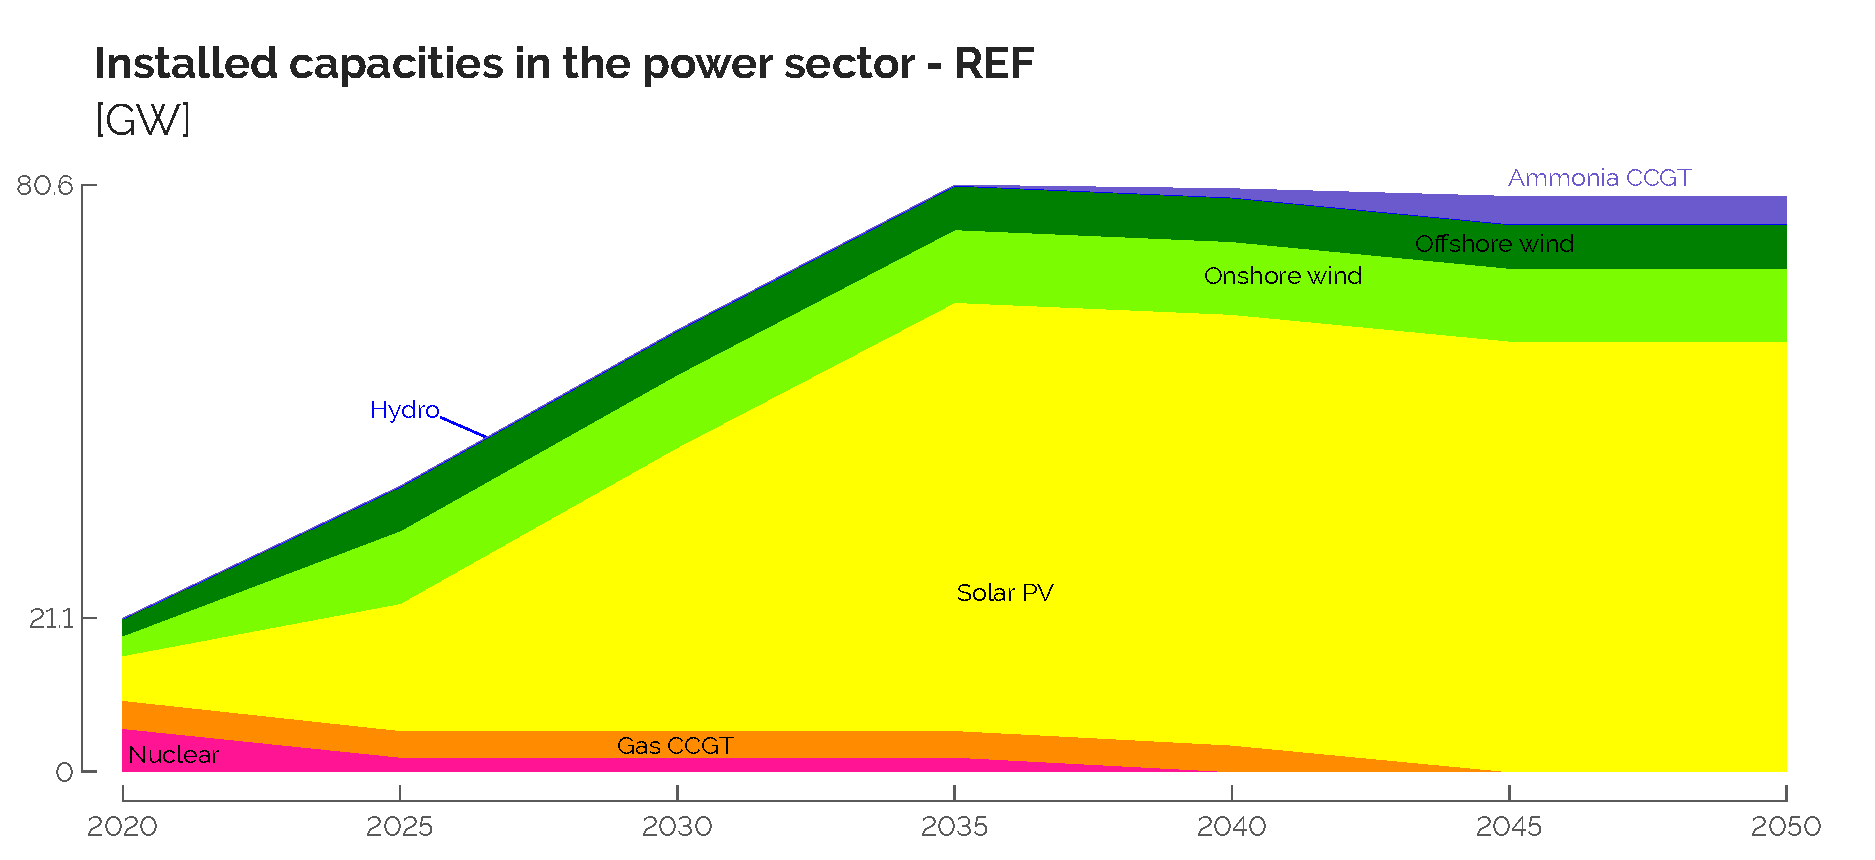
\includegraphics[width=0.49\textwidth]{figures/Elec_Tech_Cap_REF.pdf}
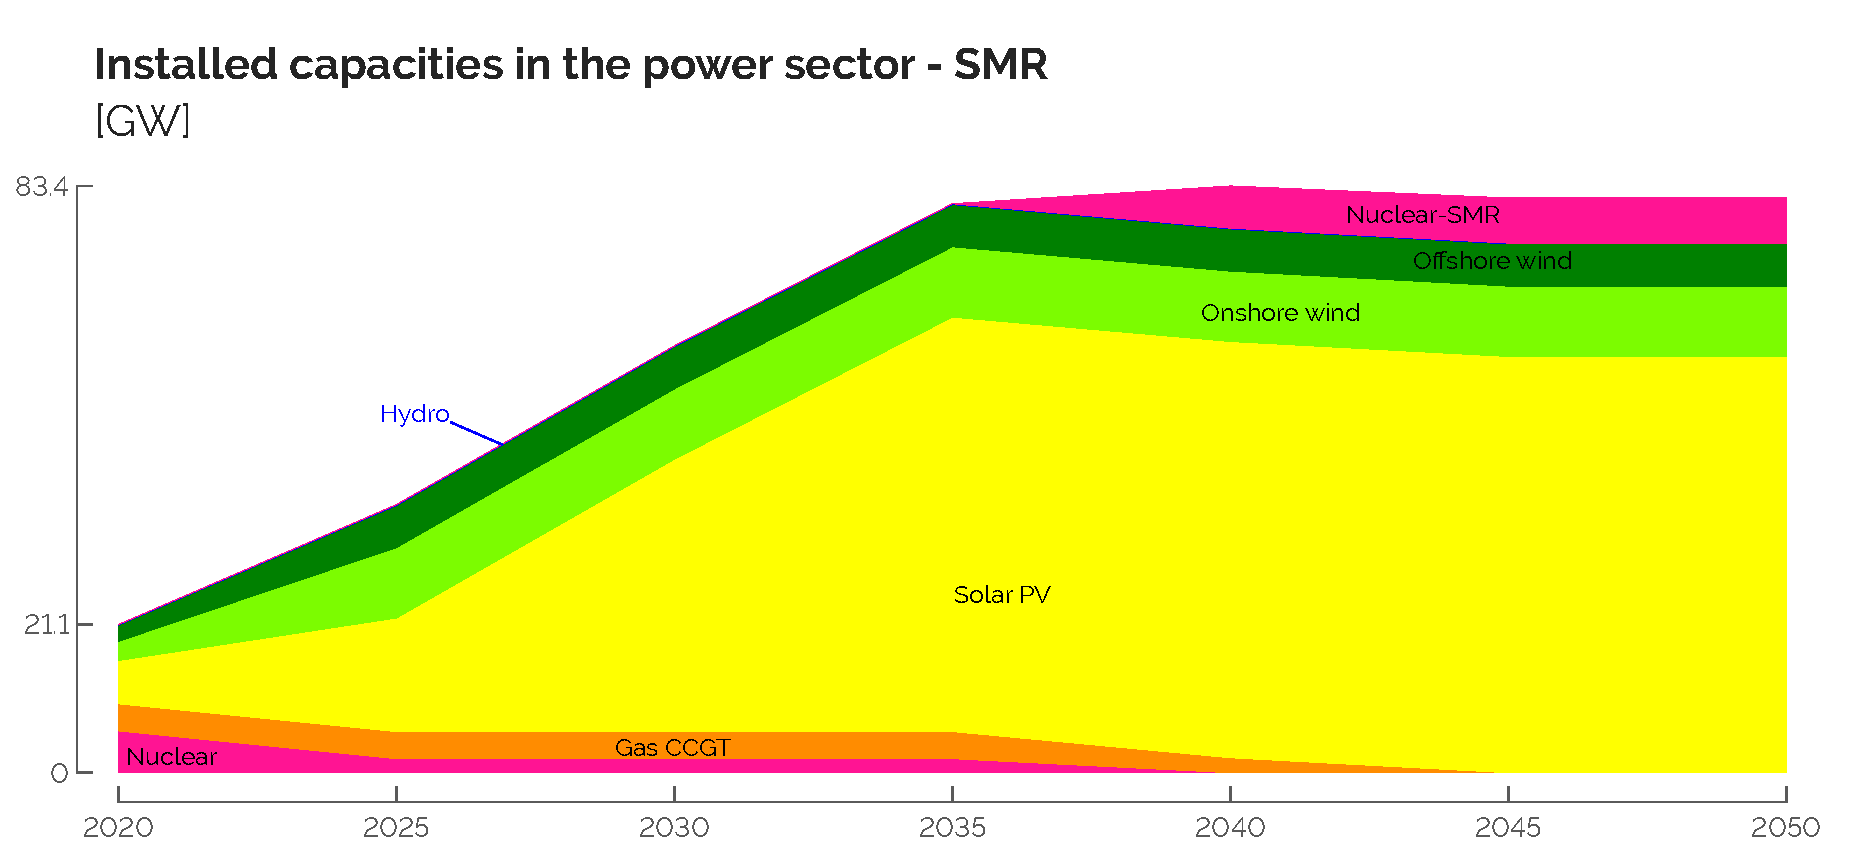
\includegraphics[width=0.49\textwidth]{figures/Elec_Tech_Cap_SMR.pdf}
\caption{As soon as available (\ie 2040), nuclear small modular reactors (SMR) are deployed to their maximum potential (\ie 6\,GW) to substitute more expensive flexible generation units (\ie gas and ammonia \gls{CCGT}). Abbreviations: \acrfull{CCGT}, \acrfull{PV}.}
\label{fig:results_deter_tech_cap_elec}
\end{figure}

When assessing the electricity production-versus-consumption-balance (\Cref{fig:results_deter_layer_elec}), nuclear SMR, as a cheap\footnote{Even though the reactor itself is a cost-intensive asset, the long lifetime assumed in this study makes it, after annualisation and discounting the salvage value in 2050, a low-cost investment. Moreover, besides the smaller energy-efficiency compared to \gls{CCGT}, the fuel to supply SMR, \ie uranium, is assumed to be up to 97\% cheaper than renewable ammonia as shown in \Cref{fig:cs_resources_cost}.}, flexible and low-emitting power generation system, produces to its full capacity, given the 15\% maintenance off-time assumed in this work: 44.6\,TWh. By 2050, it represents 24.6\% of the total electricity production which is less than the current share of conventional nuclear in Belgium, 38.5\%. This resurgence of nuclear electricity occurs at the expense of other, although more efficient technologies: \gls{CCGT} and industrial \gls{CHP}. Then, besides the unchanged end-use-demand, we observe a slight increase of the electrification of the rest of the system: +9.4\% which corresponds to +5.8\,TWh, mostly consumed by electric heaters (+48\%) to produce industrial high-temperature heat.

\begin{figure}[!htbp]
\centering
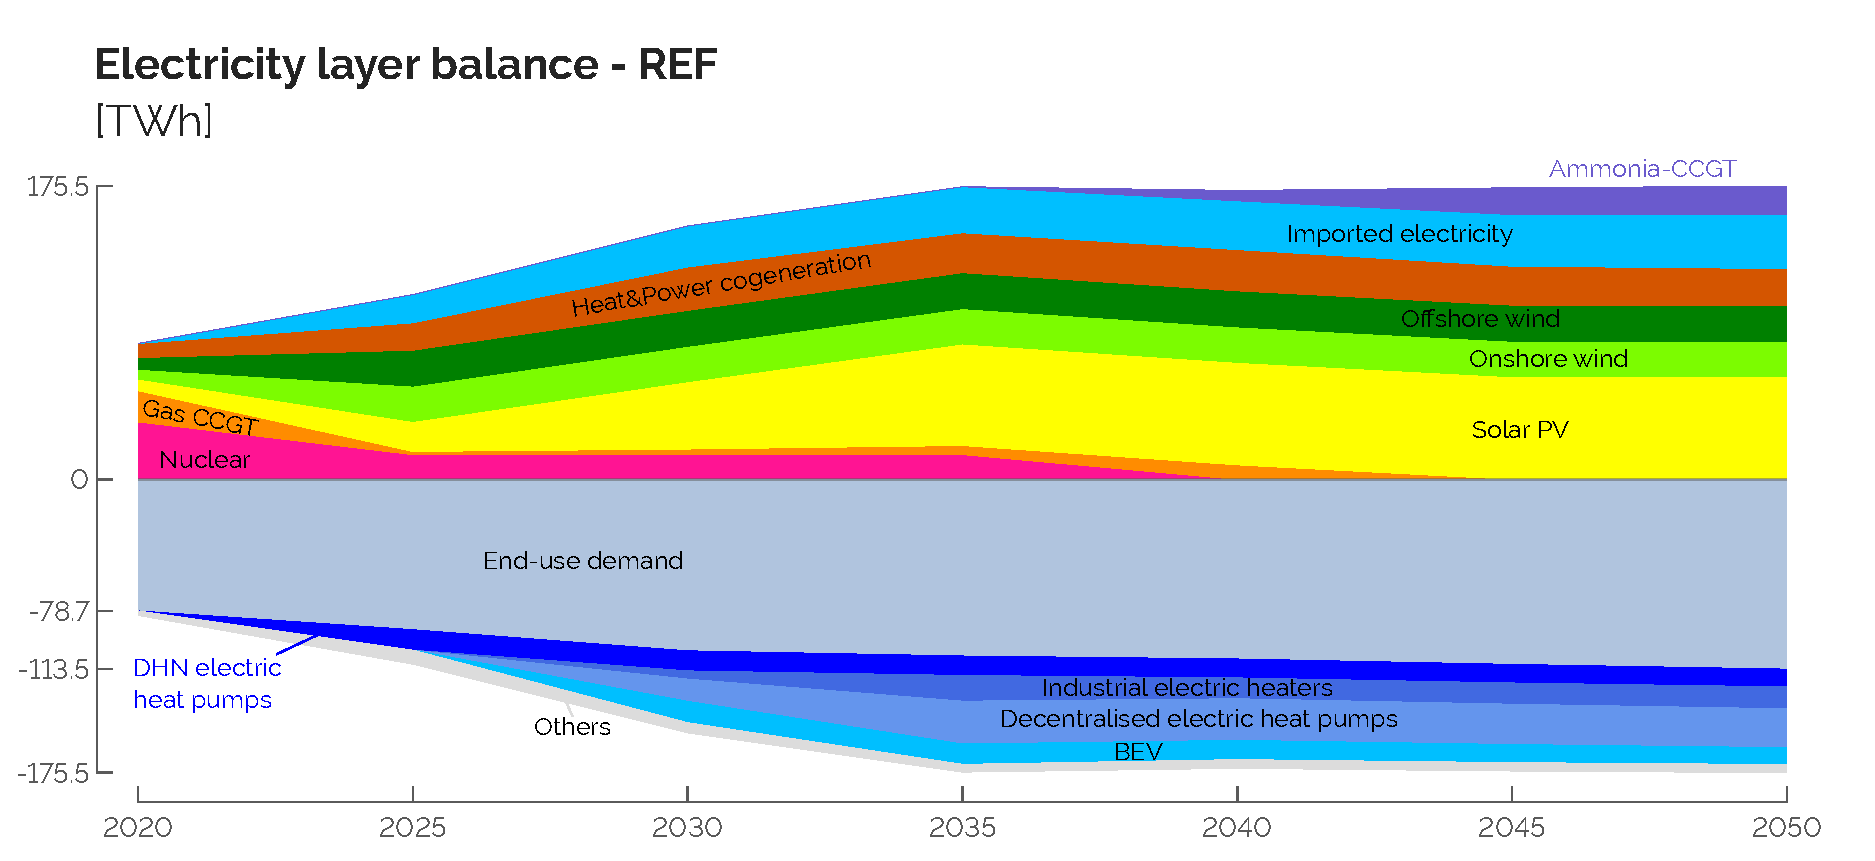
\includegraphics[width=0.49\textwidth]{figures/Elec_Layer_REF.pdf}
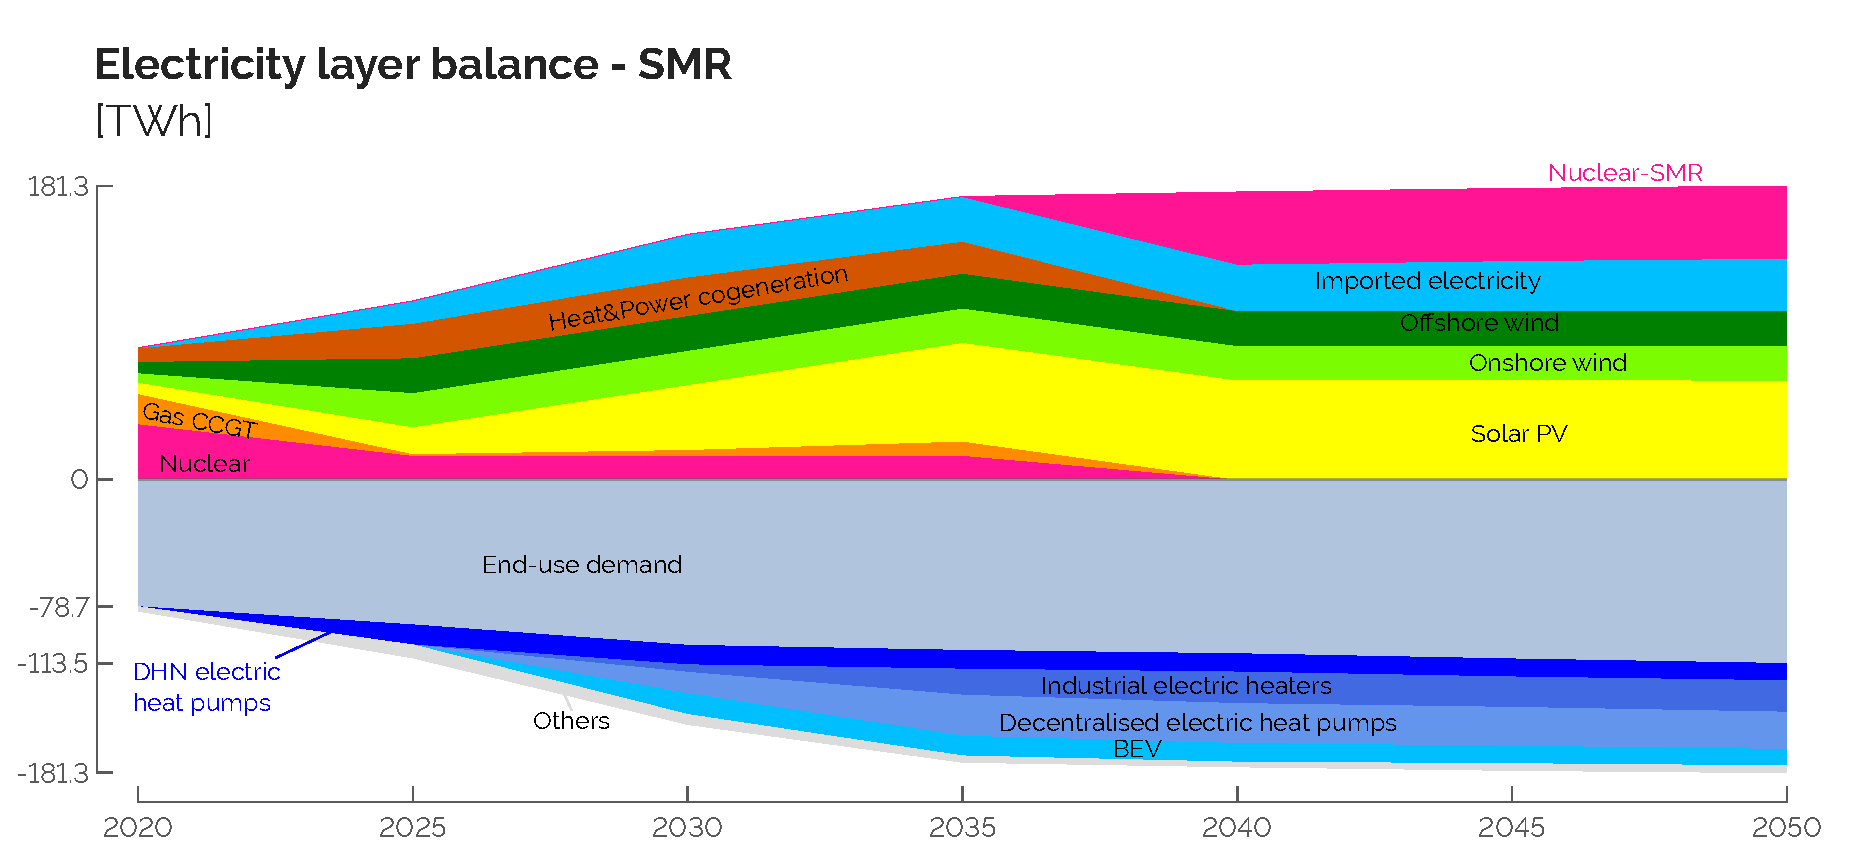
\includegraphics[width=0.49\textwidth]{figures/Elec_Layer_SMR.pdf}
\caption{The production of electricity from nuclear SMR substitutes more efficient technologies (\ie \gls{CCGT} and \gls{CHP}) and boosts the electrification of the rest of the system, mostly the industrial high-temperature heat sector. Abbreviations: \acrfull{BEV}, \acrfull{CCGT}, \acrfull{CHP}, \acrfull{DHN}, \acrfull{PV}.}
\label{fig:results_deter_layer_elec}
\end{figure}


\subsubsection{System-level impacts}
\label{subsubsec:results_deter_overall}
First of all, as far as the objective function (\ie the total transition cost) is concerned, \Cref{fig:results_deter_overall_cost} shows that the 6\,GW nuclear SMR installed from 2040 allow to reach a 36.9\,b€ (-3.3\%) cheaper overall transition. Interestingly, as the model can freely spend the constrained \ce{CO2}-budget over the transition, knowing ahead (\ie perfect foresight) that cheap and low-emitting nuke-SMR will be available in the future, cost-savings, that are more important after 2040, also occur before 2040. As explained later on, this is mostly due to the extended use of cheaper fossil fuels at the beginning of the transition. Then, the capital-intensive investments in nuclear SMR, mostly recovered by the end of the transition as salvage value, are widely compensated by the smaller resource-related opex. This leads, at the end, aggregating the opex and the annualised capex, to a system that is yearly 8.8\% less expensive by 2050.

\begin{figure}[!htbp]
\centering
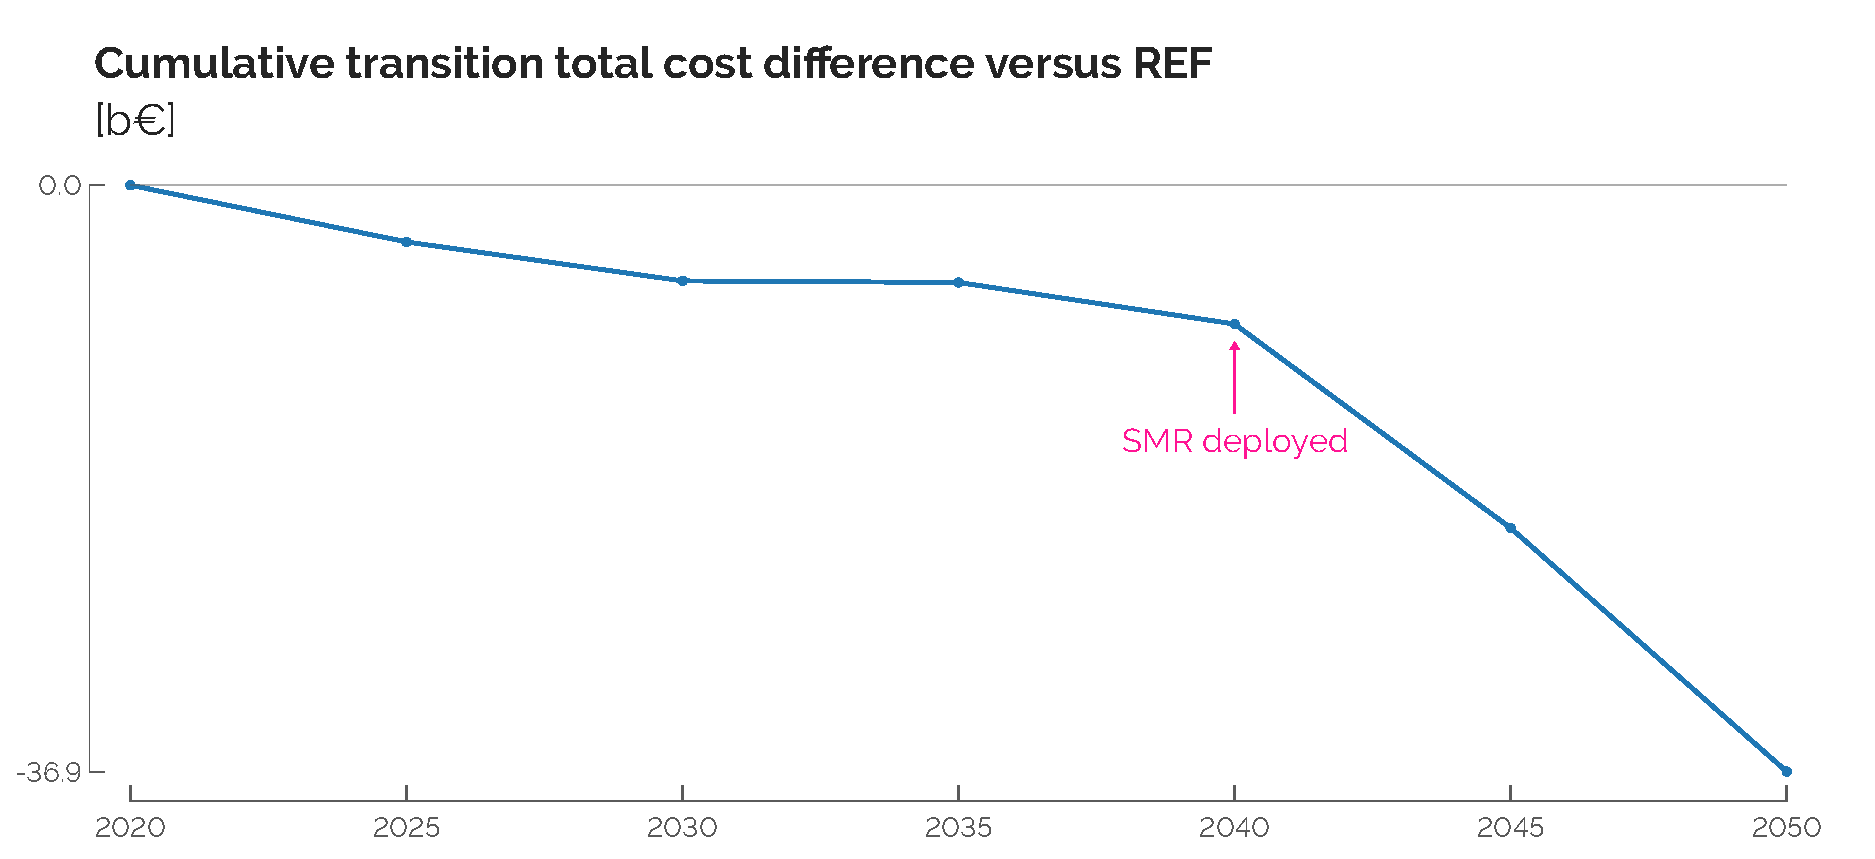
\includegraphics[width=0.6\textwidth]{figures/Cum_total_cost_diff_REF.pdf}
\caption{Cumulative transition cost difference between the SMR and the REF cases. Including nuclear SMR ends up in a cheaper overall transition (\ie -36.9\,b€, -3.3\%).}
\label{fig:results_deter_overall_cost}
\end{figure}

Then, considering the primary energy mix shown on \Cref{fig:results_deter_energy_mix}, three phases in the transition can be identified. Before 2040, thanks to the perfect foresight approach, the model finds it more economical in 2025 to keep on using 33.2\,TWh of \gls{LFO} to produce \gls{HVC} through naphtha/LPG-cracking. In 2040, uranium-driven nuclear SMR substitutes the electricity originally produced from industrial \gls{CHP} and \gls{CCGT} running respectively on fossil gas and renewable ammonia. Finally, from 2045 onward, the significant drop in the consumption of electrofuels comes from the same industrial \gls{CHP}. Here is the illustration of the atom-molecules dilemma where the consumption of local renewables are, on their side, kept as is. In other words, nuclear SMR competes with importing electrofuels while both support the integration of local solar and wind energies. Then, like the power sector, the SMR case ends up in a less efficient whole-energy system by 2050 at it consumes 47\,TWh (+12.7\%) primary energy more to supply an unchanged \gls{EUD}. Interestingly, in both cases, given the assumptions made on the \gls{GWP} of the resources (\ie $\mathit{gwp}_{\mathrm{op,electrofuels}}=0$\,kt$_{\ce{CO2},\text{eq}}$/GWh and $\mathit{gwp}_{\mathrm{op,uranium}}=0.004$\,kt$_{\ce{CO2},\text{eq}}$/GWh), the only constraint on the \ce{CO2}-budget leads to ``carbon-neutrality'' by 2050\footnote{The model being constrained to keep on using all the waste that would keep on being locally produced, the system in 2050 reaches a $\sim 3.5\,Mt_{\ce{CO2},\text{eq}}$/year.}.

\begin{figure}[!htbp]
\centering
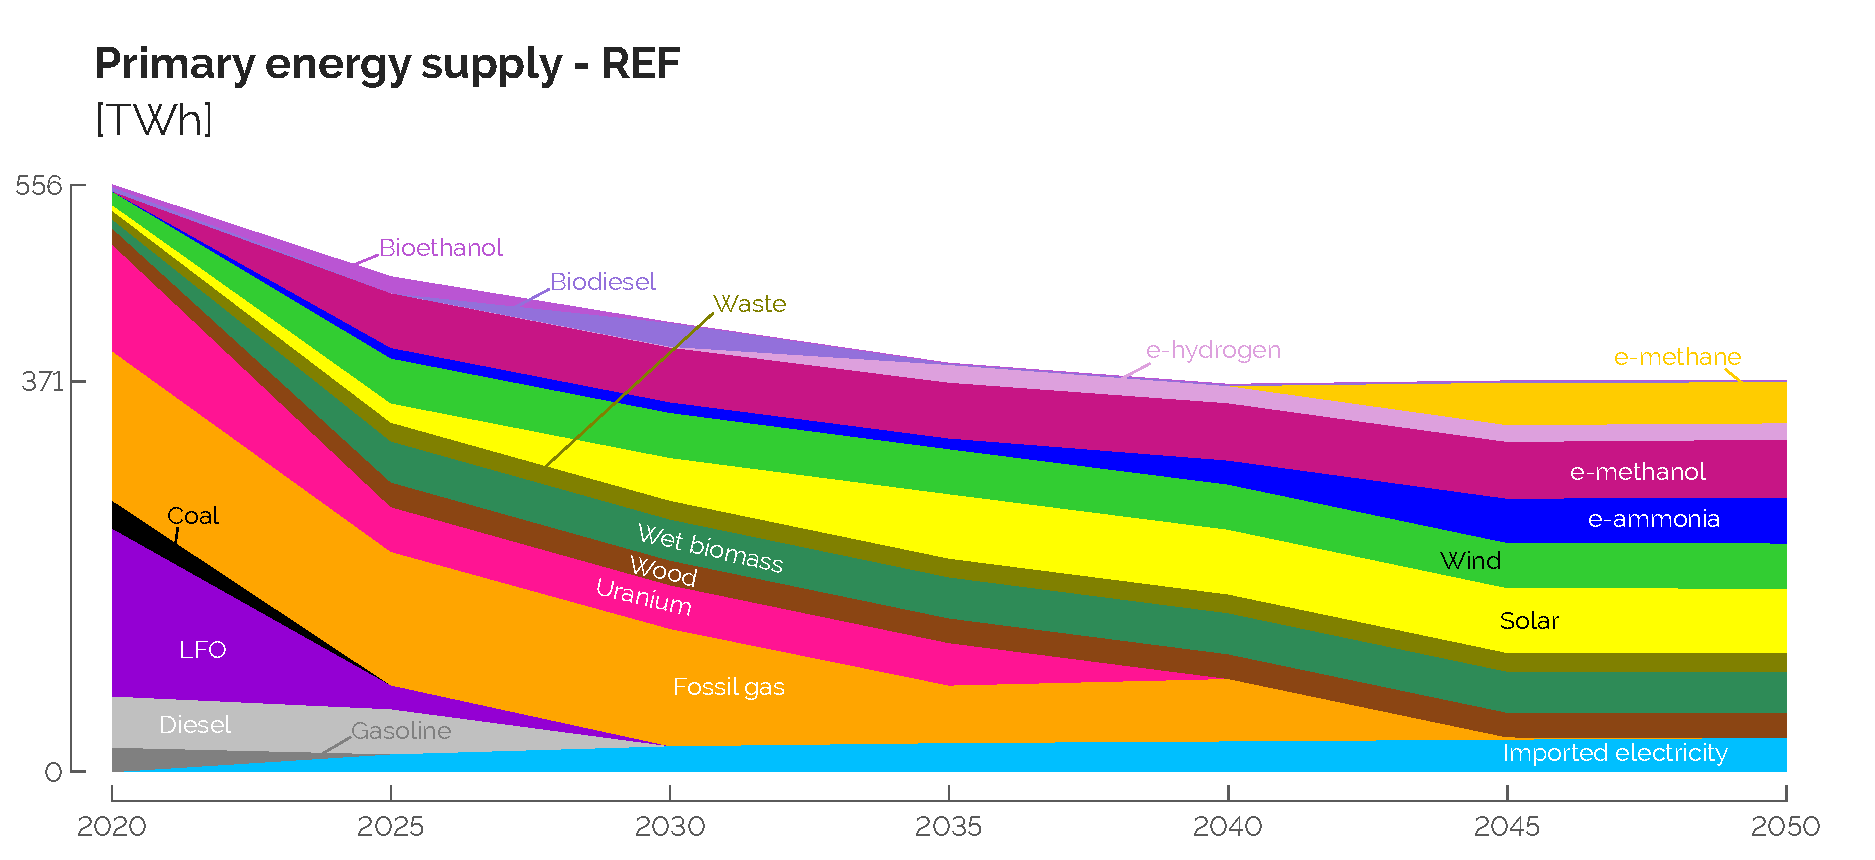
\includegraphics[width=0.49\textwidth]{figures/Primary_mix_REF.pdf}
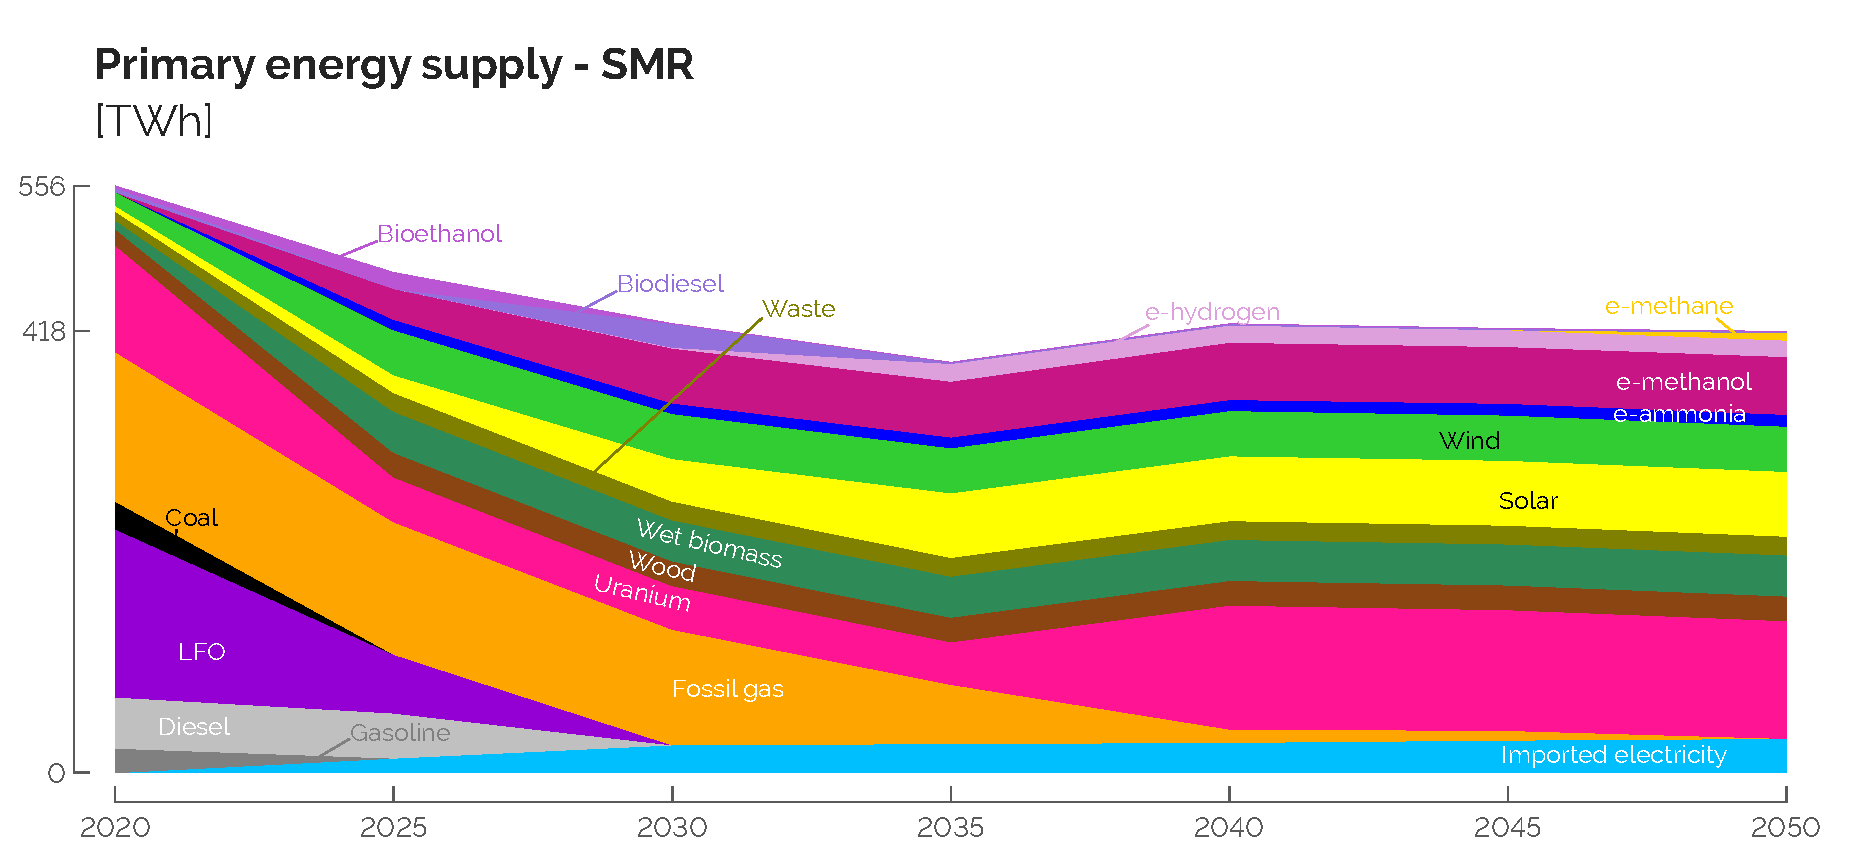
\includegraphics[width=0.49\textwidth]{figures/Primary_mix_SMR.pdf}
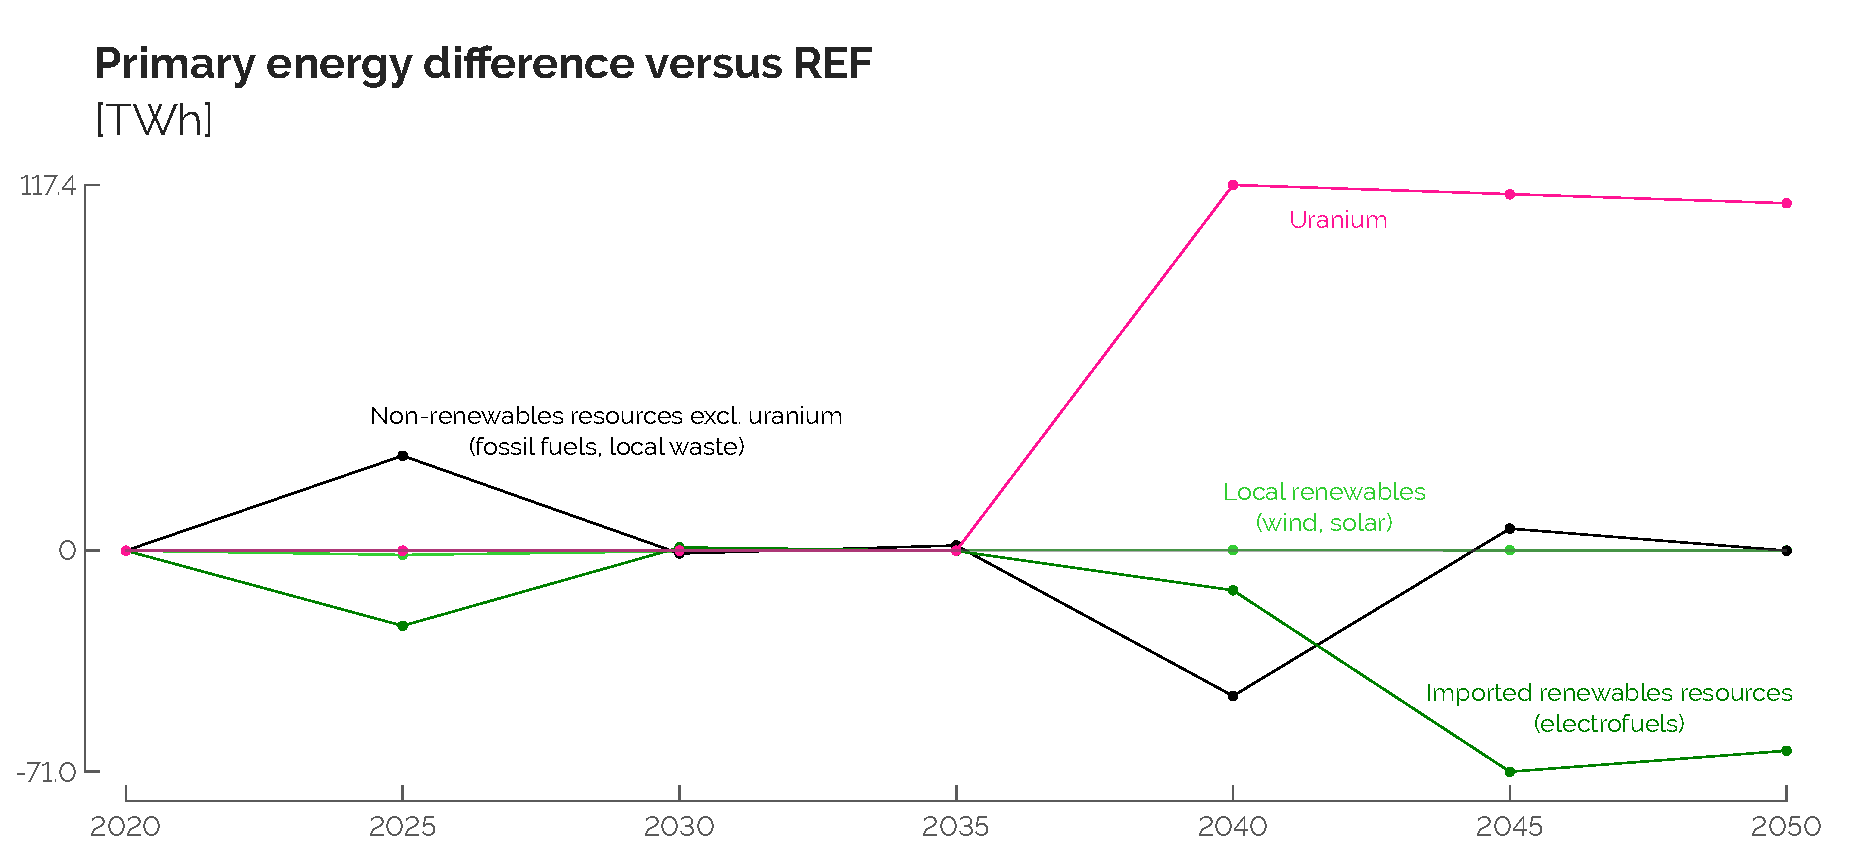
\includegraphics[width=0.49\textwidth]{figures/Primary_mix_diff_uranium.pdf}
\caption{(Top) Primary energy mix over the transition for the REF and SMR cases. (Bottom) Difference of these mix between the two cases after aggregation per category. In the latter, uranium, considered as a non-renewable resource in line with \citet{rixhon2021terminology}, is nevertheless dissociated from other non-renewable resources for the sake of clarity. The imported electricity is split between imported non-renewable and renewable resources assuming a linear decrease between the current share of renewables, \ie 37.41\% \cite{eurostat_share_re_elec}, and an assumed 100\%-renewable European electricity mix by 2050. Abbreviations: \acrfull{LFO}.}
\label{fig:results_deter_energy_mix}
\end{figure}

\subsubsection{Other non-power sectors}
\label{subsubsec:results_deter_others}
\paragraph*{High-temperature heat}
As aforementioned, the main impact of including nuclear SMR from 2040 onward on the high-temperature heat sector is (i) its higher direct electrification and (ii) the reduction of overall more efficient heat-and-power co-generation in the benefit of single-output industrial boilers. On one hand, in the REF case, industrial electric heaters are mainly used to absorb, instead of curtailing, the ``over-production" of the 59\,GW solar-PV, when fully deployed, in the sunny days. With nuclear SMR, by 2050, an additional 1.7\,GW (+13\%) of these heaters can rely on a more constant supply of defossilised electricity, consequently increasing their load factor and yearly production respectively by 31\% and 48\%. On the other hand, given the 44.6\,TWh of electricity produced by nuclear SMR, cogeneration units are less relevant and, by 2050, 2.6\,GW industrial gas boilers completely substitute \gls{CHP} to produce 16.6\,TWh (\ie 23\% of the total production of high-temperature heat).

\paragraph*{Low-temperature heat}
This sector is marginally impacted. In both cases, the major shift of supply from decentralised to centralised productions operates early in the transition, to hit the constraint that \gls{DHN} can not supply more than 37\% of the \gls{LT}-heat production. Then, from a mix between oil (53\%), gas (43\%) and wood (4\%) boilers for the decentralised production of \gls{LT}-heat in 2020, the system progressively shifts towards only electric \gls{HP}. Similarly, the most efficient and economic option for the centralised production.

\paragraph*{Mobility}
The passenger mobility is not affected neither as the electrification of the system is initially favoured towards this sector with \gls{BEV} progressively substituting \gls{ICE} cars for the private sector. About the public mobility, trains and tramways supply their \textit{a priori} set maximum share, respectively, 50\% and 30\% complemented by \gls{CNG} buses substituting diesel-driven buses. Similarly, considering the freight transport, technology shifts (\ie from diesel to \gls{FC} trucks) or modal shares (\ie 53\%-47\% split between \gls{NG} and (bio)-diesel boats) are identical between the two cases.

\paragraph*{Non-energy demand}
The supply of ammonia (\ie from Haber-Bosch to direct import of renewable ammonia) and methanol (\ie import of renewable methanol) are unchanged between the two cases. However, as introduced previously, to produce \gls{HVC}, the full substitution of naphtha/LPG-cracking by \gls{MTO} is delayed as the emissions of the former are compensated by the later integration of nuclear SMR.

\subsection{Uncertainty quantification on the cost, the atom and the molecules}
\label{subsec:results_uq}
``\textit{It is difficult to make predictions, especially about the future.}" (Niels Bohr). Consequently, besides the deep understanding of the deterministic results, it is important to challenge these conclusions out-of-sample, accounting for the uncertainty of the parameters. To mitigate the computational burden, we have then used the \gls{PCE} approach (see \Cref{subsec:meth:UQ}) on the monthly version of EnergyScope Pathway. As detailed by \citet{limpens2023pathway}, this simplified model does not implement daily storage technologies and integrates much more easily intermittent renewables (PVs and wind turbines) in the system as the daily supply-demand intermittency and mismatch are not at stake. Although, it allows to quantify the full set of 34 uncertain parameters (\ie 1260 samples for an order-2 \gls{PCE}) in an hour, and avoid the computation burden of the hourly pathway (\ie roughly two weeks for the same number of runs). Nevertheless, comparing the \gls{UQ} on the hourly pathway with a limited set of uncertain parameters and on the monthly model, Appendix \ref{app:UQ_transition_cost} shows that the most impacting parameters are correctly captured by the latter.

After briefly assessing the \gls{GSA} on the main output of the model, the total transition cost, this section keeps on investigating the atom-molecules dilemma, using the same samples of uncertain parameters. This time, the Sobol' indices will be computed for import of renewable molecules and installed capacities of nuclear SMR.

\subsubsection{Total transition cost}
\label{subsubsec:results_uq_cost}
Exhaustively listed in Appendix \ref{app:UQ_transition_cost}, \Cref{tab:UQ_short} gathers the most impacting parameters\footnote{Per \citet{Turati2017}, parameters are considered as ``impacting'' if their Sobol' index is above the threshold $=1/d$, $d$ being the total number of uncertain parameters after the pre-selection phase. In this case, $d=34$, and, consequently, the threshold is equal to 2.9\%.} on the total transition cost, highlighting the cost of purchasing of electrofuels as well as the potentiality to install nuclear SMR and its capex. The former is the most impacting parameter whereas the two others have much more negligible influence on the variation of the total transition cost. Given the uncertainty characterisation presented in Section \ref{subsubsec:UQ:UC}, there are 60\% chance that no nuclear SMR could be installed. Moreover, given its characteristics detailed in \Cref{tab:SMR_features}, mostly its cheap and low-emitting fuel (\ie uranium) and the long lifetime leading to lower annualised capex and higher salvage value, this explains why nuclear SMR has this limited impact. In the contrary, more expensive renewable electrofuels are always imported, to a smaller or larger extent depending on the sample. For instance, in the REF case (see Section \ref{subsubsec:results_deter_overall}), the imported electrofuels represent, by 2050, 152.9\,TWh (\ie 41\% of the primary energy mix) with an average 93€/MWh cost of purchasing and, over the entire transition, a 273\,b€ cumulative opex (\ie 25\% of the total transition cost).

\begin{table}[htbp]
\caption{Total Sobol' indices of the uncertain parameters over the total transition cost. Where the cost of purchasing of electrofuels is the top-1 parameter, nuclear SMR-related parameters have a negligigble impact on this cost. Abbreviations: \acrfull{EUD}.}
\label{tab:UQ_short}
\centering
\begin{tabular}{l c c}
\toprule
\textbf{Parameter}  & \textbf{Ranking} & \textbf{Sobol' index} \\	
\midrule
\textbf{Purchase electrofuels} & 1 & 47.4\% \\
Industry EUD & 2 & 23.5\% \\
Interest rate & 3 & 11.0\% \\
Purchase fossil fuels  & 4 & 6.9\% \\
$\vdots$ & $\vdots$ & $\vdots$\\
\textbf{Potential capacity nuclear SMR} & 11 & 0.9\% \\
$\vdots$ & $\vdots$ & $\vdots$\\
\textbf{Capex nuclear SMR} & 32 & $<$0.1\% \\
\bottomrule							

\end{tabular}
\end{table}

Given the relatively wide uncertainty range (\ie up to [-30.8\%; +24.0\%] by 2050) and, above all, the major share among the total demand, between 53\% and 60\%, the industrial \gls{EUD} is the second most impacting parameter. Then, as the driving factor for the annualisation and the salvage value of the assets, the interest rate has a 11\% Sobol' index. Finally, similarly to electrofuels, the cost of purchasing of fossil fuels is also to consider in the perspective to reduce the uncertainty over the total transition. However, due to the ambitious \ce{CO2}-budget, phasing out of fossil fuels is urgent and makes their uncertain impact smaller than their renewable alternatives.

\subsubsection{Atom and molecules}
The samples used to carry out the \gls{GSA} on the total transition cost, also provide the distribution of other outputs of the model. Among them, \Cref{fig:results_uq_electrofuels} shows the evolution of the import of renewable electrofuels over the transition. Appendix \ref{app:UQ_electrofuels} gives a more detailed information. On one hand, it compares the statistics features (\ie quartiles and median) with these values in the REF and SMR cases. On the other hand, this appendix shows the distributions of the different sources of supply and consumption of gas, hydrogen, ammonia and methanol.

As the general trends are increasing, discrepancies exist between the different energy carriers. E-methane, as the renewable alternative to fossil natural gas, substitutes it, sometimes at a very early stage of the transition, 2025, and to a somehow unrealistically large extent, 173\,TWh, which is more than 13\% more than the total import of electrofuels in the REF case. The necessity to import this molecule is progressive through the transition to supply mostly industrial \gls{CHP} and boilers. 

E-hydrogen becomes rapidly the main stream of hydrogen in the system, on top of steam-methane-reforming or electrolysis, to reach a median and a maximum values of, respectively 13.6\,TWh and 40.7\,TWh in 2050. Hydrogen is more frequently used in the mobility sector. Like in the REF case, fuel cell trucks are often the first option but, in some outlying cases, fuel cell cars and buses appear to completely substitute respectively \gls{BEV} cars and \gls{CNG} buses by 2050. Moreover, some samples lead to local production of methanol via the methanolation process, to produce up to 16.3\,TWh of methanol (\ie 30\% of the total supply of methanol of the nominal REF and SMR cases). 

Then, the import e-ammonia, becoming rapidly cost-competitive against its fossil alternative (see \Cref{fig:cs_resources_cost}), quickly substitutes it and the Haber-Bosch process. Where the initial purpose of ammonia is to satisfy a relatively limited \acrfull{NED} (\ie 10 $\pm$ 3\,TWh by 2050), the variation of its import is mostly due to the higher or lower need for ammonia-\gls{CCGT} as a flexible option to produce electricity. From 2035, out of the four considered electrofuels, the import e-ammonia is the one exhibiting the largest uncertainty with, for instance, an interquartile range (IQR)\footnote{The interquartile range is the difference between the third quartile ($Q3$ or $P_{75}$) and the first ($Q1$ or $P_{25}$). It is an indicator of statistical dispersion around the median, $Q2$ or $P_{50}$.} of about 50\,TWh. In some extreme cases, e-ammonia is the most imported molecules, \ie up to 233\,TWh or 63\% of the total primary mix in the REF case in 2050. 

Likewise, e-methanol early becomes the selected option to supply methanol even though alternatives like biomass-to-methanol or synthetic methanolation exist in some outlying cases. Its own \gls{NED} being even smaller (\ie 1.5$\pm$0.5\,TWh by 2050), the variation of imported e-methanol is almost exclusively due to its role in the industrial production of \gls{HVC}, \ie 78\% of the total \gls{NED}, through the \acrfull{MTO} process. In some rare samples, methanol is also used to supply the freight transport sector via boats or trucks.

\begin{figure}[!htbp]
\centering
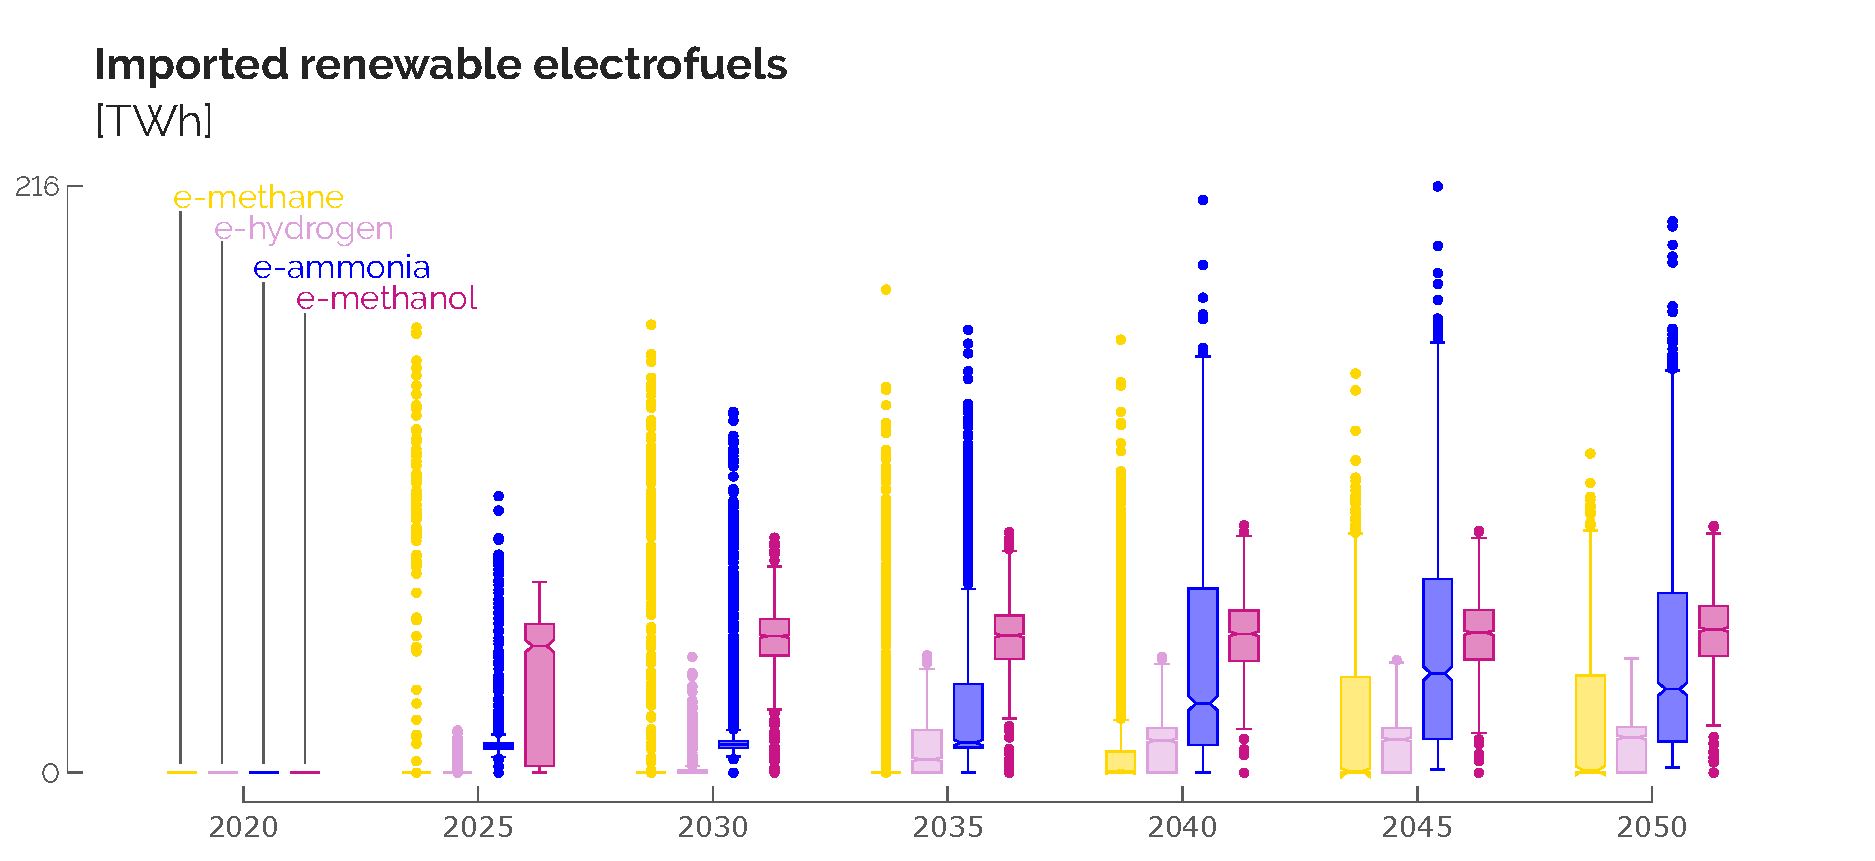
\includegraphics[width=0.6\textwidth]{figures/UQ_Electrofuels.pdf}
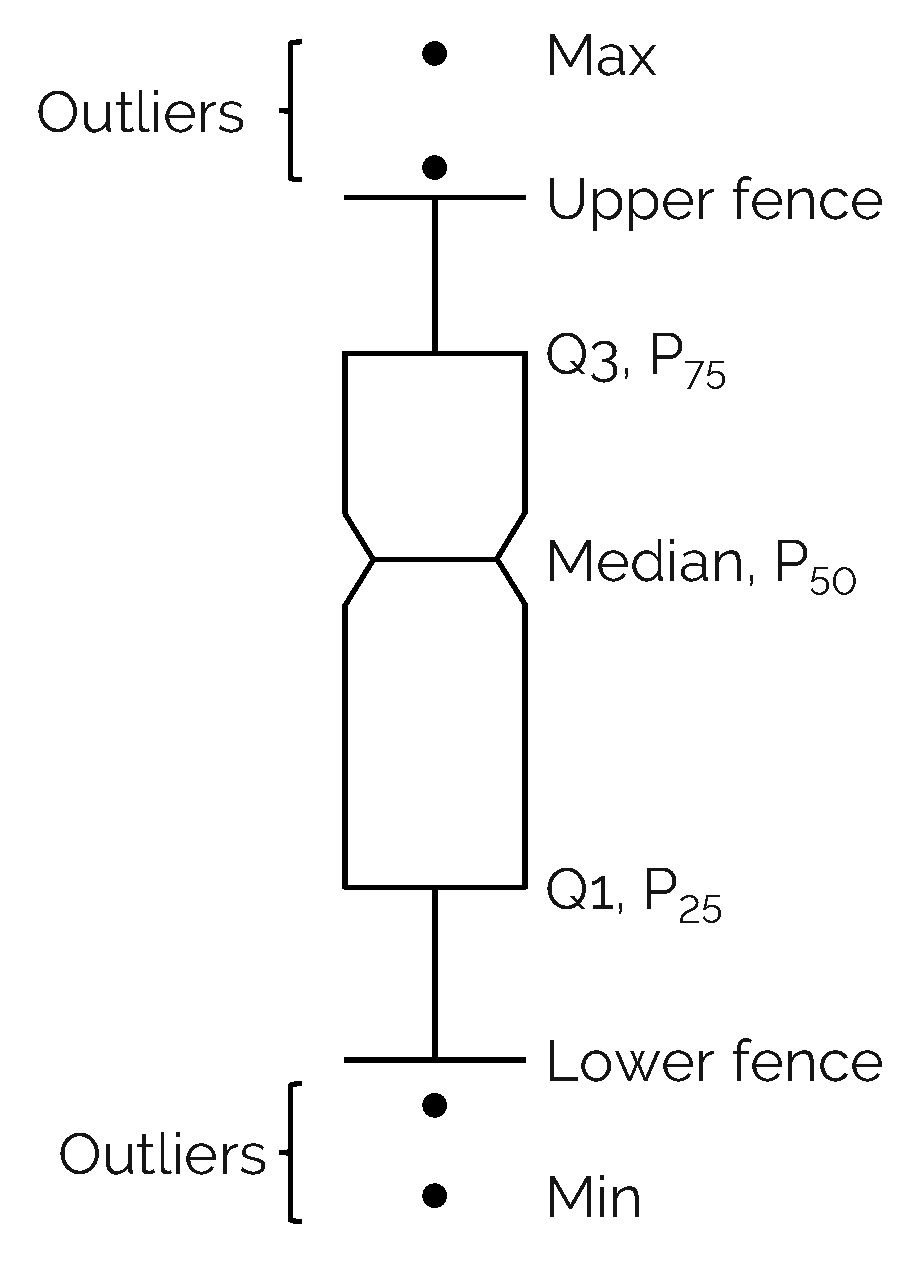
\includegraphics[height=4cm]{figures/Schematic_boxplot.pdf}
\caption{Distribution of the imported renewable electrofuels over the transition. Starting from no electrofuel in 2020, their respective import rises progressively along the transition (\ie increasing median) at different growth rates and with different ranges of values. Outliers are defined as is if the observation is either 1.5 times the interquartile range less than the first quartile (Q1) or 1.5 times the interquartile range greater than the third quartile (Q3).}
\label{fig:results_uq_electrofuels}
\end{figure}

After investigating the distribution of imports of the electrofuels over the transition, this part assesses the uncertain space of uncertainties, like \citet{pickering2022diversity} who investigated the space of feasibility to reach carbon neutrality in Europe. \Cref{fig:results_uq_samples} highlights the top- and bottom-15\% of the samples, out of the 1260 ones of the \gls{GSA}, for these imports in 2050\footnote{The authors picked this specific year as it is the one where electrofuels, if imported, are imported in the largest amount, in general, compared to the other years of the transiton.}, as well the installed capacities of nuclear SMR. Where the bottom line of the each figure gives the corresponding total transition cost, the middle rows give the parameters impacting the most the output of interest in the first row. Next to the name of a parameter, one can read its Sobol' index versus the output of interest\footnote{For these output of interest, differement from the total transition cost, the \gls{LOO} error is generally higher than the threshold of \SI{1}{\%} defined in Section \ref{subsubsec:UQ:PCE}. Consequently, the Sobol' indices are less accurate but already allow a fair relative comparison between the different comparison.}. The values of each row are normalised between their respective minimum and maximum values. Diamonds give an indication of the values taken by the different features in the REF (green), the SMR (pink) or both (orange) cases.

As aforementioned, the industrial \gls{EUD} impacts the most the import of e-methane. The tipping-point being roughly the nominal value, this parameter directly dictates the demand of industrial high-temperature heat for which industrial gas \gls{CHP}, and industrial gas boilers to a lower extent, represent, on average over all the samples, respectively 25.6\% and 6.1\% of the total production. Then, considering the smaller-impact parameters, we notice that nuclear SMR plays a non-negligible role. Indeed, if deployed and combined with a much lower industrial \gls{EUD}, nuclear SMR produces abundant low-emitting electricity for industrial electric heaters that substitute, even completely, gas alternatives. This confirms the observation made in Section \ref{subsubsec:results_deter_others}. 

As far as e-hydrogen is concerned, besides the cost of purchasing of the electrofuels, the higher the less are the imports of e-hydrogen, the driving parameters are mostly related to the transport sector. As shown on \Cref{fig:results_uq_prod_cons} in Appendix \ref{app:UQ_electrofuels}, the more frequent use of hydrogen in the system is the \gls{FC} trucks, then, to a lower extent, \gls{FC} cars and buses. The former supplies, on average, 63.5\% of the total road freight transport. Consequently, the higher is the capex of fuel cell engines, the less the system imports e-hydrogen. This goes the same way with the cost of purchasing of the electrofuels. Then comes the cost of purchasing of the biofuels as the third most impacting parameter. As the mostly picked alternative to \gls{FC} trucks, those running on biodiesel provides, on average, 27.6\% of the total. To a smaller extent, behind the \gls{CNG} buses that drive 34.9\% of the passengers in the public road transport, \gls{FC} buses provide 11.2\% against biodiesel and hybrid biodiesel buses accounting respectively for 27.8\% and 26.1\%. Finally, the last noticeable parameter at stake is the capex of electric motors. In competition with \gls{BEV} that stand for 83.4\% on average of the private mobility sector, the cheaper these motors are, the more cost-competitive are these vehicles, and vice versa, versus \gls{FC} cars (\ie 13.7\% of the total passenger mobility, on average).

As already pointed out in Section \ref{subsubsec:results_deter_power_sector}, the installation of nuclear SMR drastically reduces the import of e-ammonia. As ammonia \gls{CCGT} is the biggest consumer of ammonia by the end of the transition, low-emitting and cheap electricity flexibly produced by nuclear SMR substitute the \gls{CCGT}. With higher cost of purchasing of the electrofuels, this import of e-ammonia drops down to 7.3\,TWh, 83.4\% less than in the REF case. Then, with a 9\%-Sobol' index, industrial \gls{EUD} also influences the need for this molecule, due to its \gls{NED}.

Eventually, the conclusions are more straightforward for the import of e-methanol and the installed capacity of nuclear SMR. For the former, industrial \gls{EUD} is, by far (\ie 81\% Sobol' index), the key factor. Due to its own \gls{NED} but, above all, since it is the low-emitting alternative picked by the model to supply the significant \gls{NED} of \gls{HVC}, the lower this demand, the lower the need to import e-methanol, and vice versa. For the latter, it is the availability of the technology that drives its installation. The pink diamond highlights this 60\% threshold below which no nuclear SMR is deployable. Surprisingly, the [-40\%; +44\%]  variation of its capex has a negligible impact, with a Sobol' index of 0.9\%.

\begin{figure}[!htbp]
\centering
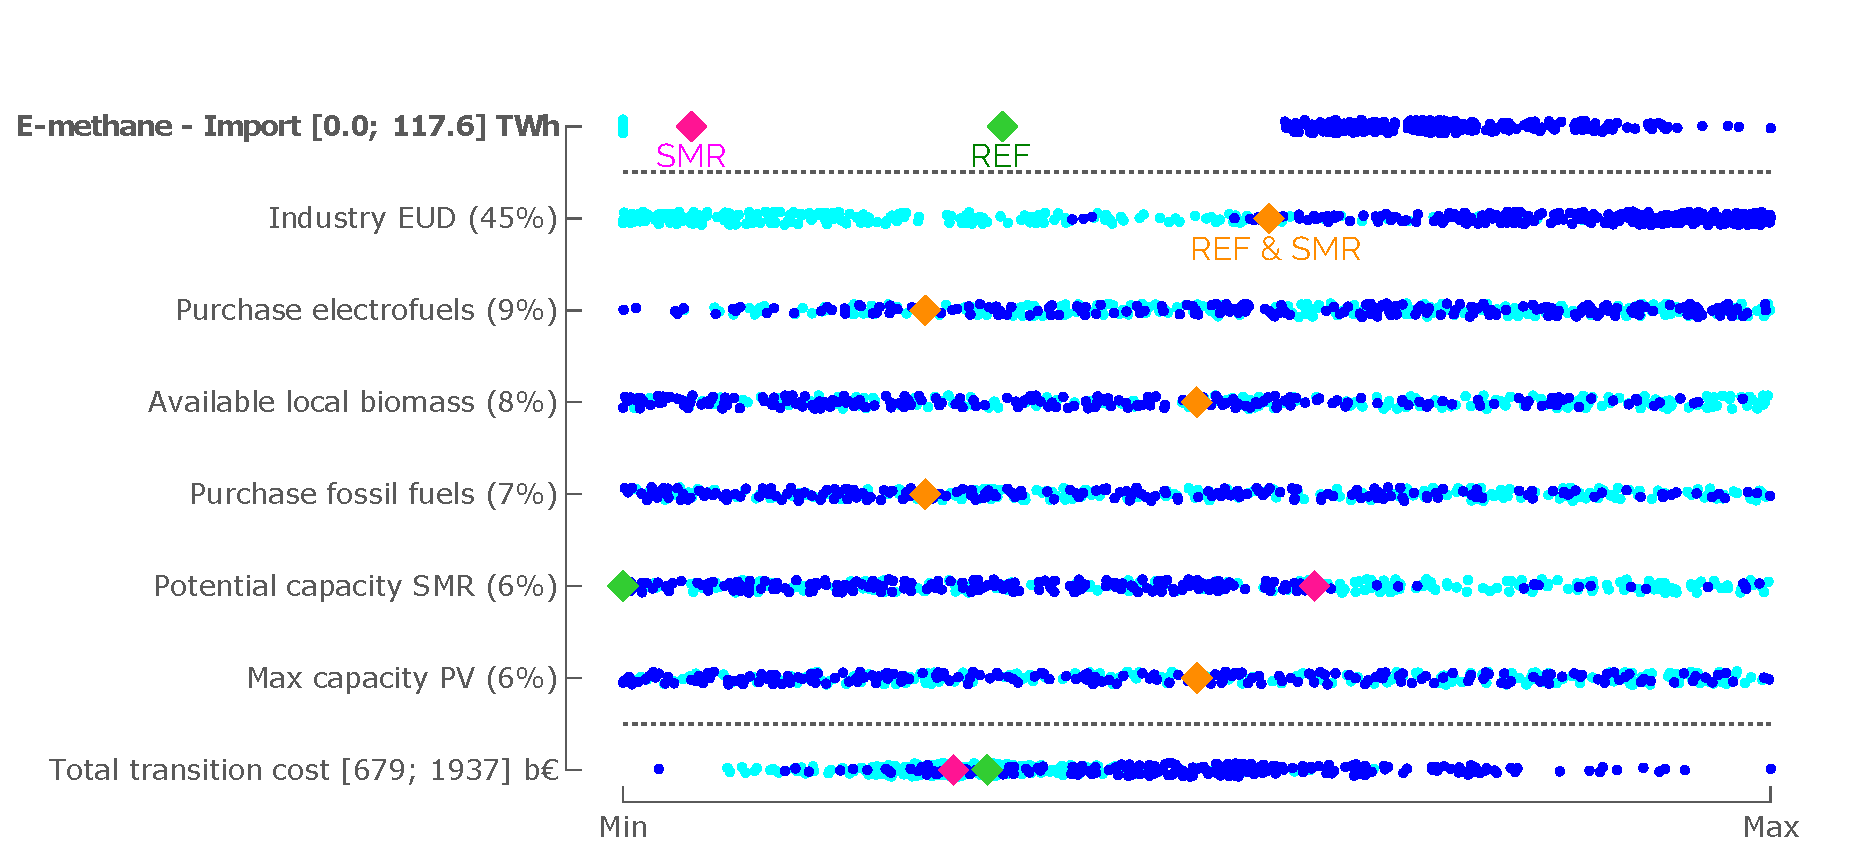
\includegraphics[width=0.49\textwidth]{figures/UQ_Gas_samples.pdf}
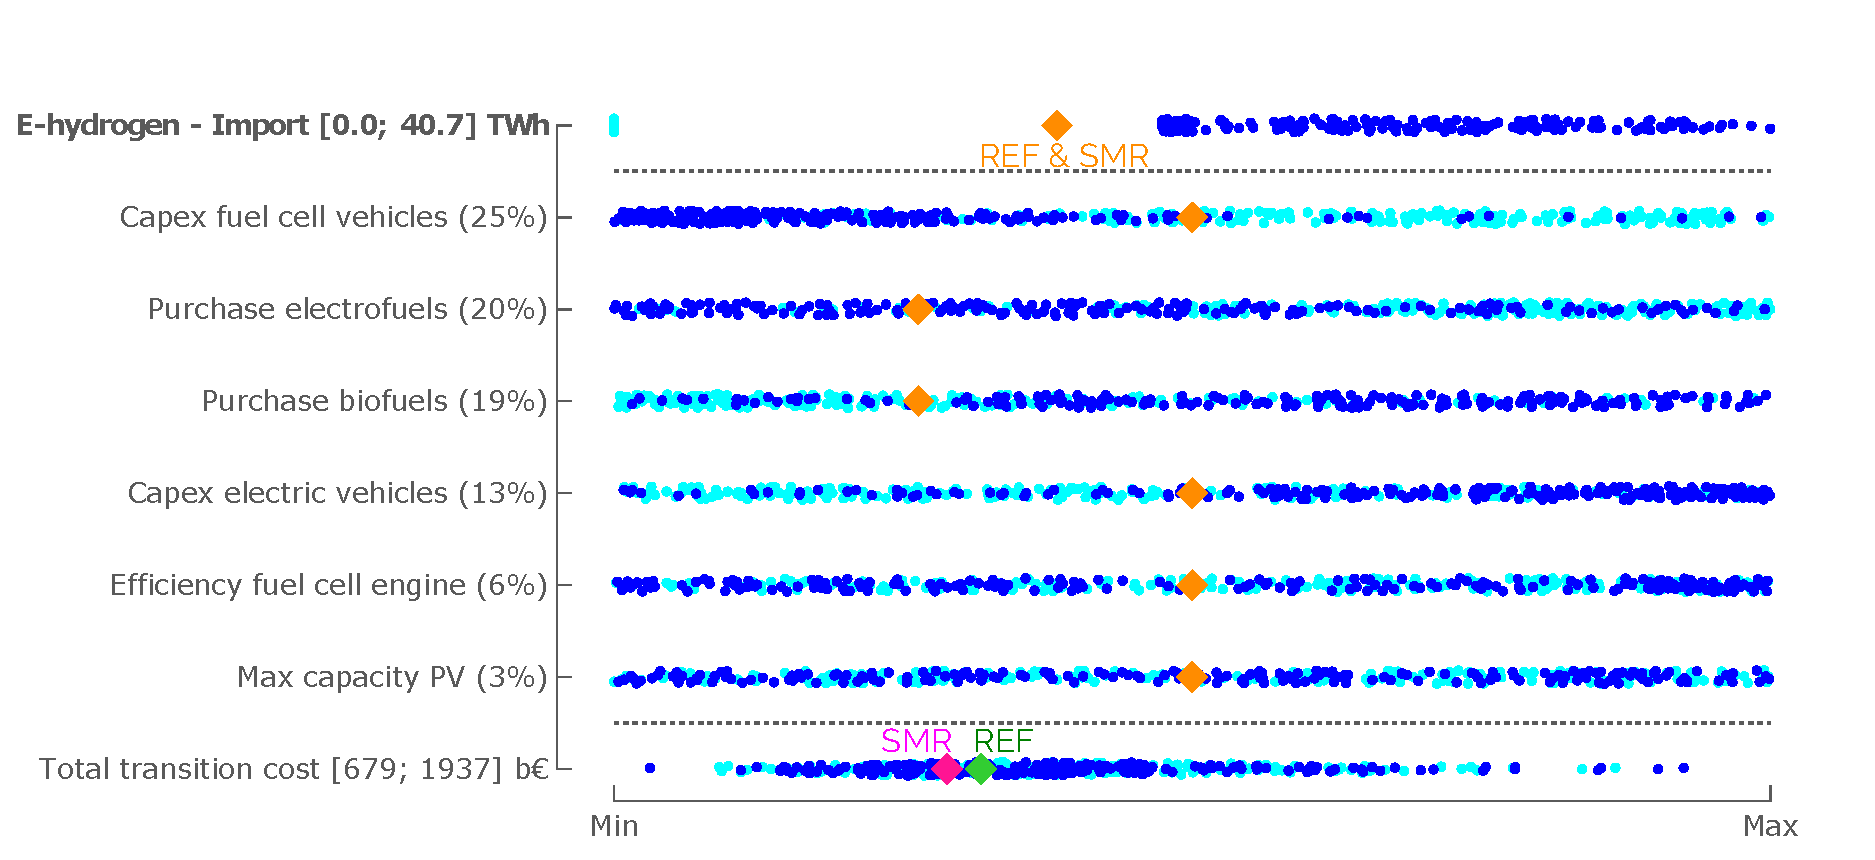
\includegraphics[width=0.49\textwidth]{figures/UQ_H2_samples.pdf}
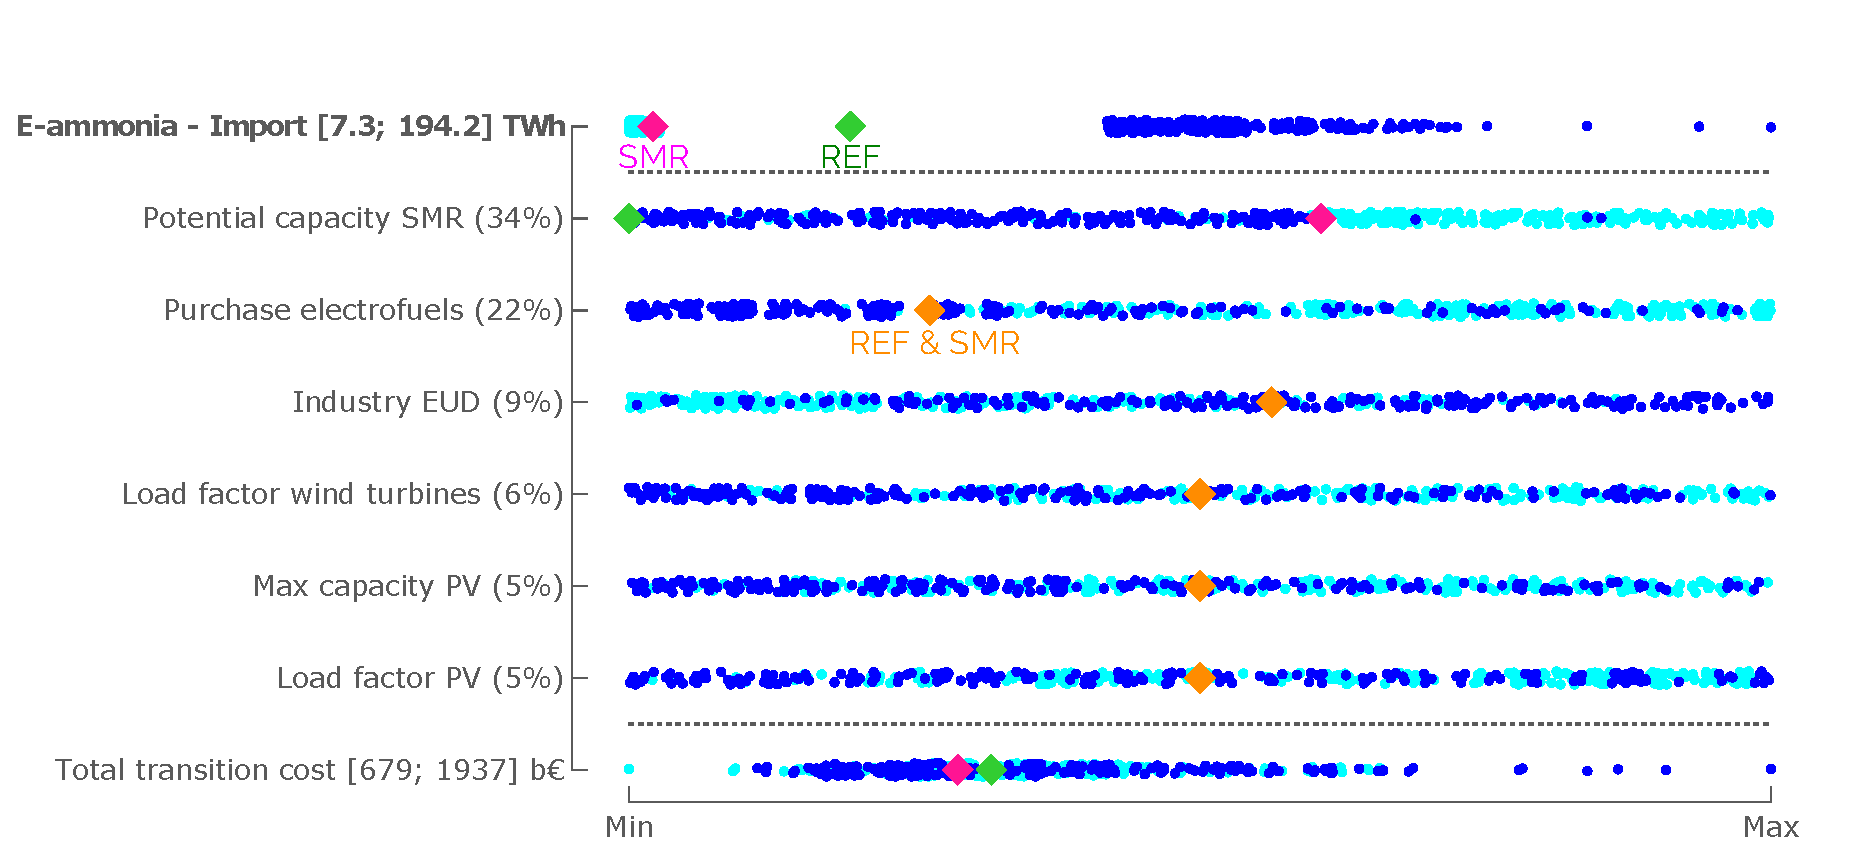
\includegraphics[width=0.49\textwidth]{figures/UQ_Ammonia_samples.pdf}
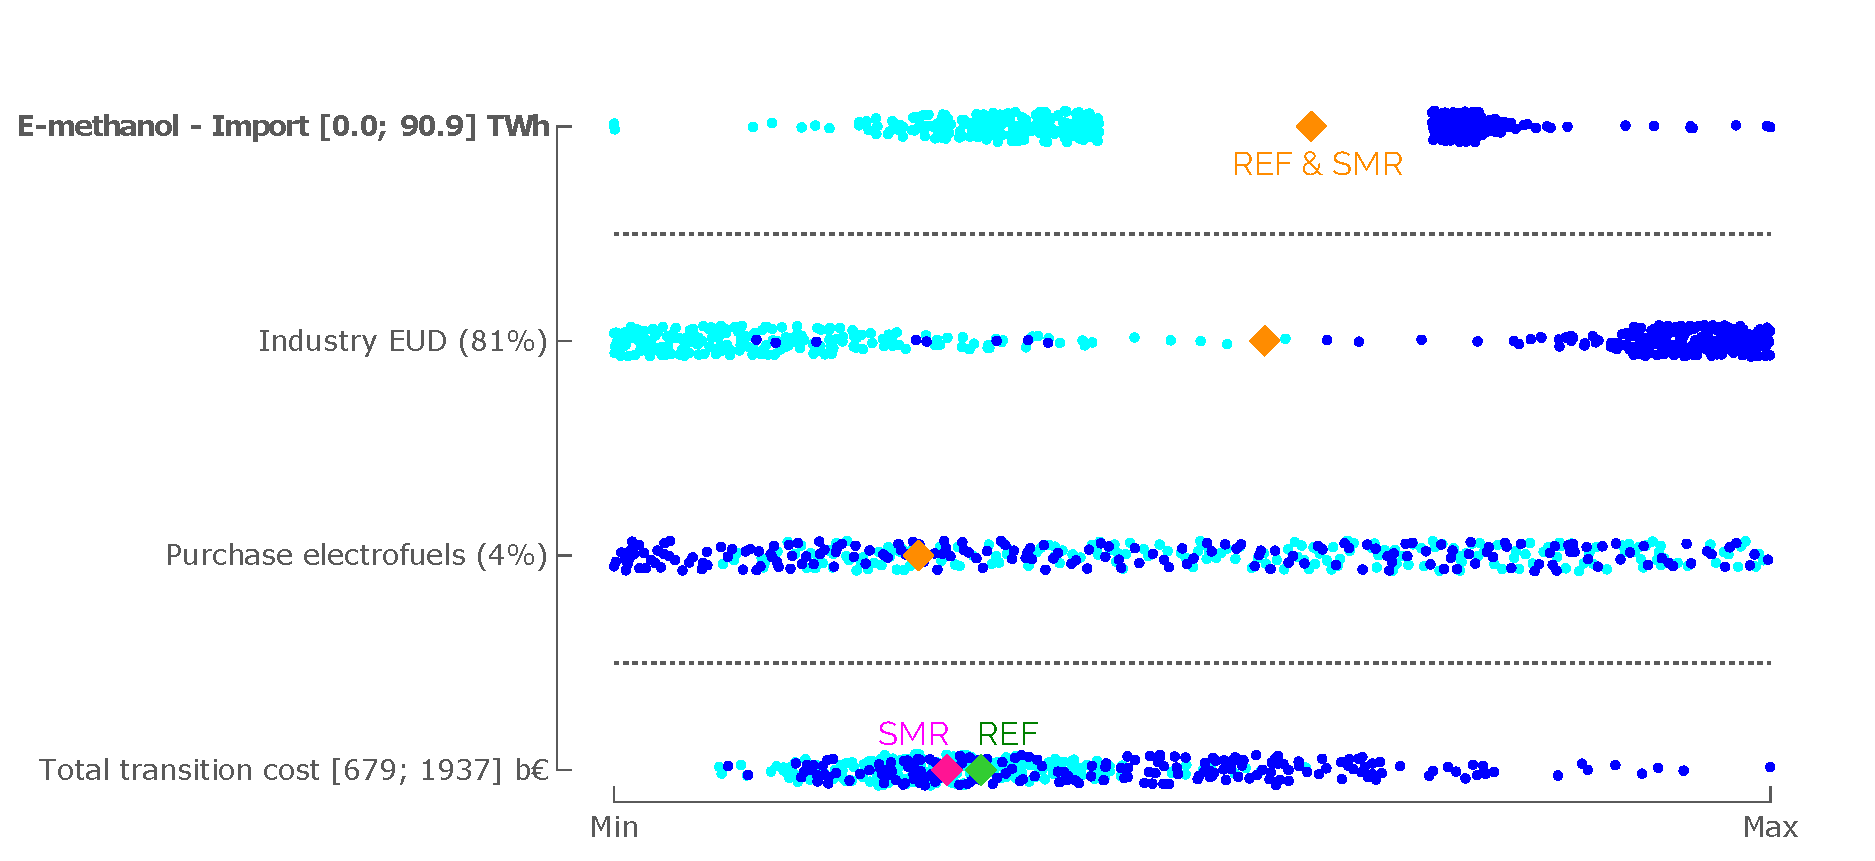
\includegraphics[width=0.49\textwidth]{figures/UQ_Methanol_samples.pdf}
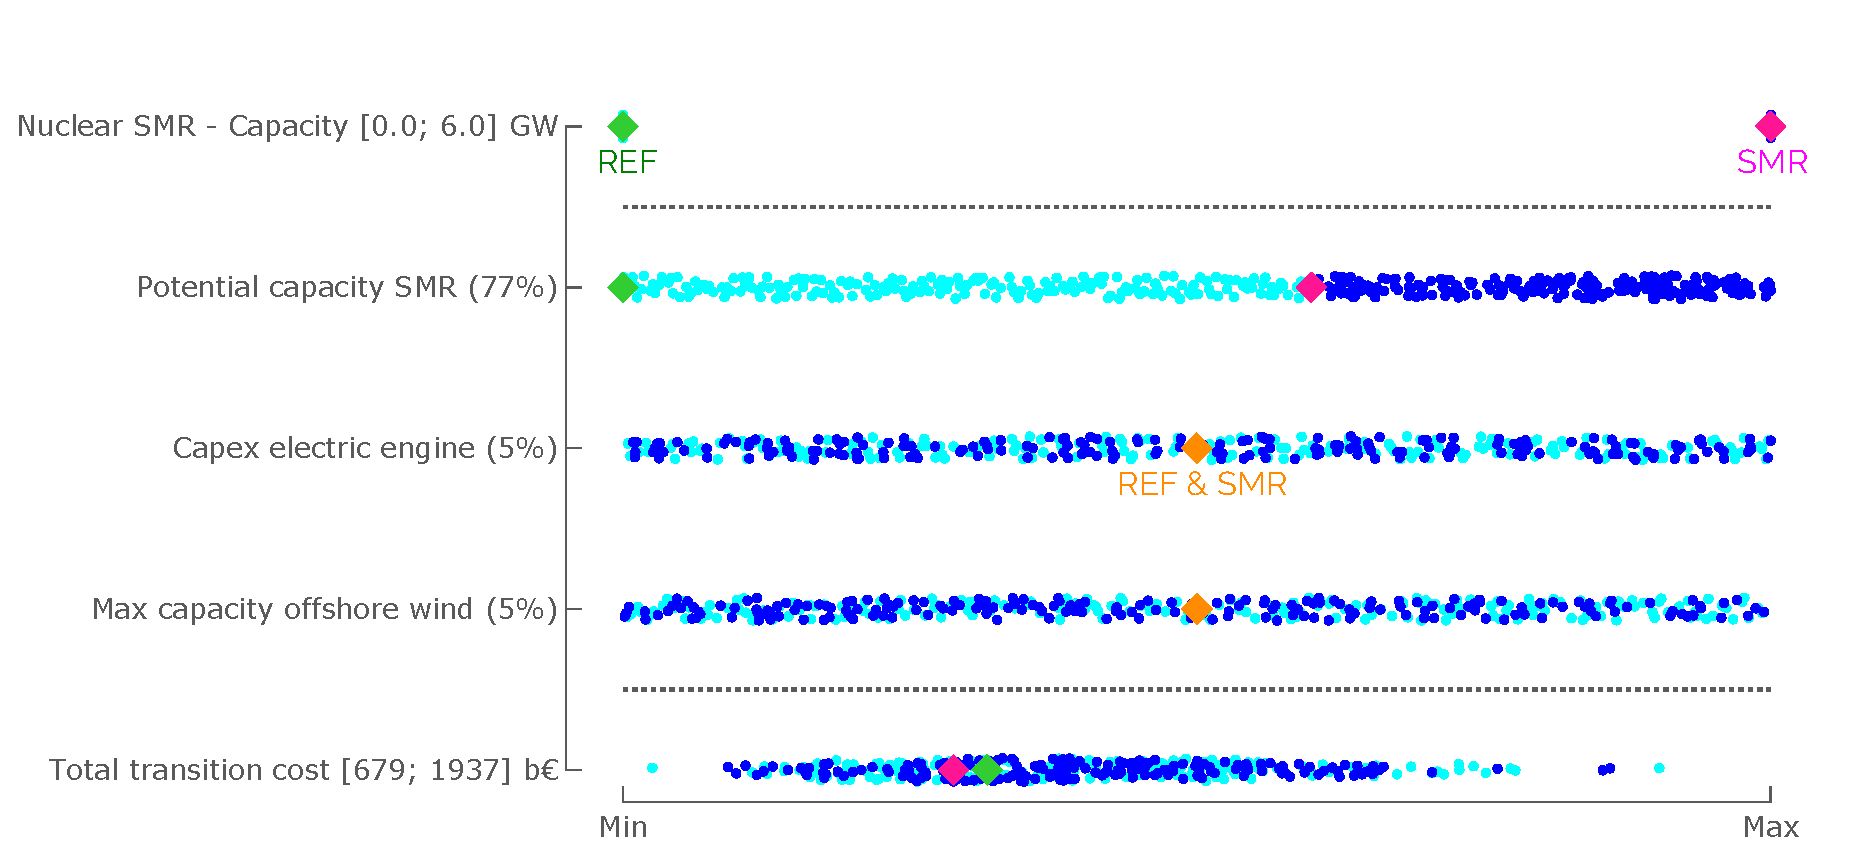
\includegraphics[width=0.49\textwidth]{figures/UQ_SMR_samples.pdf}
\caption{Out of the 1260 samples of the \gls{GSA}, samples leading, in 2050, to the top-15\% (dark blue) and bottom-15\% (cyan) of the import of e-methane, e-hydrogen, e-ammonia and e-methanol and the installed capacity of nuclear SMR. In the middle rows, are the parameters impacting the most the considered output of interest, with their indicative Sobol' index between brackets. Finally, in the bottom line, are the corresponding total transition costs. The values of each row are normalised between their respective minimum and maximum values. Green and pink diamonds represent the value of the related feature in, respectively, the REF and SMR cases. The diamonds are orange when the nominal value is identical for both of these cases. Abbreviations: \acrfull{EUD}, \acrfull{PV}.}
\label{fig:results_uq_samples}
\end{figure}

%%%%%%%%%%%%%%%%%%%%%%%%%%%%%%%%%%%%%%%%%%%%%%%%%%%%%%%%%%%%%%%%%%%%%%%%%%%%%%%%%%%%%%%%%%%%%%%%%%%%%%%%%%%%%%%%%%%%%%%%%%%%%           CONCLUSION %%%%%%%%%%%%%%%%%%%%%%%%%%%%%%%%
%%%%%%%%%%%%%%%%%%%%%%%%%%%%%%%%%%%%%%%%%%%%%%%%%%%%%%%%%%%%%%%%%%%%%%%%%%%%%%%%%%%%%%%%%%%%%%

\section{Conclusions and discussions}
\label{sec:conclusion}
\textbf{Quid autre que techno-economic Nucléaire-SMR?}
\textbf{Quid demande plus faible?}
\textbf{Quid importation massive de molécules}
Hervé Kempf - \url{https://www.seuil.com/ouvrage/le-nucleaire-n-est-pas-bon-pour-le-climat-herve-kempf/9782021512922}

\begin{itemize}
    \item Other dimensions to consider: societal, etc.
    \item Reducing the demand. Refer to Hugo Baudson
    \item Will we be able to import as many molecules as we need? Refer to \cite{lefebvre2022electrofuel}.
\end{itemize}

Parier sur l'arrivée du SMR peut être considéré comme une fuite vers l'avant quant à l'abandon des ressources fossiles, (to a smaller extent) ralentir le déploiement du renouvelable local, vers moins de sector coupling (moins de CHP), Less efficiency

A significant decrease on the demand-side is probably one of the cornerstones of the energy transition \cite{millward2020providing, contino_sobriety}.

comparaison avec \cite{heuberger2018impact} et \cite{PATHS2050}

Relying on nuclear would not especially increase our national self-sufficiency, in the contrary (more import of energy in general, by 2050)

Discussion on the \ce{CO2}-budget allocated to Belgium that could/should be lower to allow other countries in development reaching the floor of the donuts (donuts theory) $-->$ reducing the demand?

\textbf{Further works}
\begin{itemize}
    \item Quid si on attend (same strat jusque 2040) et que finalement, il n'arrive jamais. Quel serait le surcoût? La surconso d'électrofuels. Intéressant de mettre en place une policy robuste pour parer cette éventualité, surtout étant donné la vision plus myopique des choses $-->$ Reinforcement learning
    \item Limit the import of electrofuels, at least the beginning of the transition, as well as limit the import of fossil fuels by the end of it
    \item Analyse what the system looks like in the extreme cases where the imports are massive
\end{itemize}


\begin{appendices}
%%%%%%%%%%%%%%%%%%%%%%%%%%%%%%%%%%%%%%%%%%%%%%%%%%%%%%%%%%%%%%%%%%%%%%%%%%%%%%%%%%%%%%%%%%%%%%%%%%%%%%%%%%%%%%%%%%%%%%%%%%%%%           APP SOA 		 %%%%%%%%%%%%%%%%%%%%%%%%%%%%%%%%
%%%%%%%%%%%%%%%%%%%%%%%%%%%%%%%%%%%%%%%%%%%%%%%%%%%%%%%%%%%%%%%%%%%%%%%%%%%%%%%%%%%%%%%%%%%%%%
\section{Belgian energy system in 2020}
\label{sec:app:bel_2020}The Belgian whole-energy system of 2020 was largely based (88.6\% of the primary energy mix) on \og conventional fuels\fg (\ie oil and oil products (38.2\%), natural gas (29.5\%), uranium (16.3\%) and solid fossil fuels (4.6\%) while the rest mainly accounts for 26.7\,TWh of lignocellulosic and wet biomass, 12.8\,TWh of wind and 5.1\,TWh of solar \cite{spf_economy_2022}. Given the data available in the literature (mostly for the power sector) and, when not available, following the assumptions made by \citet{Limpens2020}, \Cref{tab:Belgium_2020} gives the major technologies used in 2020 to supply the different demands of \Cref{fig:cs_demands}.

\begin{table}[htbp]
\caption{Major technologies used to supply the 2020-demands of \Cref{fig:cs_demands} in terms of share of production and installed capacity. $^{(a)}$ The decentralised heating units provide 98\% of the low-temperature heat demand. $^{(b)}$ The private mobility accounts for 80\% of the passengers mobility. Abbreviations: \acrfull{CCGT}, \acrfull{CHP}, \acrfull{CNG}, decentralised (DEC), \acrfull{DHN}, \acrfull{HEV}, passenger (pass.), temperature (Temp.).}
\label{tab:Belgium_2020}
\begin{minipage}{\linewidth}
\centering
\begin{tabular}{l c c c}
\toprule
\multirow{2}{*}{\textbf{End-use demand}} & \textbf{Major} & \textbf{Share of} & \textbf{Installed}\\
    &	 \textbf{technology} 	& \textbf{supply} & \textbf{capacity}	 \\ 	
\midrule							
\multirow{3}{*}{Electricity}
 & Nuclear & 39\% & 5.9\,GW\\
 & CCGT & 21\% & 3.9\,GW\\
 & Wind turbines & 14\% & 5.0\,GW\\
\midrule
\multirow{3}{*}{Heat High-Temp.}
 & Gas boiler & 36\% & 3.3\,GW\\
 & Coal boiler & 30\% & 2.3\,GW\\
 & Oil boiler & 20\% & 1.5\,GW\\
\midrule
\multirow{3}{*}{Heat Low-Temp. (DEC)$^{(a)}$}
 & Oil boiler & 48\% & 21.4\,GW\\
 & Gas boiler & 40\% & 17.5\,GW\\
 & Wood boiler & 10\% & 4.4\,GW\\
\midrule
\multirow{3}{*}{Heat Low-Temp. (DHN)}
 & Gas CHP & 59\% & 0.3\,GW\\
 & Gas boiler & 15\% & 0.3\,GW\\
 & Waste CHP & 15\% & 0.1\,GW\\
\midrule
\multirow{2}{*}{Private mobility$^{(b)}$}
 & Diesel car & 49\% & 93.5\,Mpass.-km/h\\
 & Gasoline car & 49\% & 94.7\,Mpass.-km/h\\
 & HEV & 2\% & 5.9\,Mpass.-km/h\\
\midrule
\multirow{3}{*}{Public mobility}
 & Diesel bus & 43\% & 3.6\,Mpass.-km/h\\
 & Train & 43\% & 3.9\,Mpass.-km/h\\
 & CNG bus & 5\% & 0.8\,Mpass.-km/h\\
\midrule
\multirow{3}{*}{Freight mobility}
 & Diesel truck & 74\% & 62.7\,Mt.-km/h\\
 & Diesel boat & 15\% & 10.8\,Mt.-km/h\\
 & Train & 11\% & 2.5\,Mt.-km/h\\
\midrule
HVC & Naphtha/LPG cracking & 100\% & 4.6\,GW\\
Ammonia & Haber-Bosch & 100\% & 1\,GW\\
Methanol & Import & 100\% & -\\
\bottomrule							
\end{tabular}
\end{minipage}
\end{table}

\section{Uncertainty characterisation} 
\label{app:UC_full}
Table \ref{tab:UC_full} summarises the uncertainty ranges for the different groups of technologies and resources, for the year 2025. Refer to \cite{Moret2017, Moret2017PhDThesis} for the methodology and sources. As the model optimises the system every 5 years, $N=5$ has been selected to get the final ranges of uncertainties of type II and III, based on the work of \citet{Moret2017PhDThesis}. For type III uncertainties (\ie uncertainty ranges increasing with time), a 50\% increase has been set arbitrarily between the ranges for 2025 and these same ranges for 2050. In other words, for these specific uncertainties, the ranges for 2050 are 50\% larger than for 2025.

\citet{rixhon2021role} analysed the impact of these parameters on the total cost of the snapshot Belgian whole-energy system in 2050 subject to different \gls{GWP} limits. Based on this work, we have selected a subset of impacting uncertainties, added others due to the pathway formulation (\eg $\Delta_{\mathrm{change,pass}}$), and listed them in Table \ref{tab:UC_full}. The uncertainty characterisation gives the uncertainty ranges per parameter or group of parameters (category). Indeed, some parameters are correlated \textit{a priori}, such as the cost of purchasing of fossil fuels or the cost of vehicles running on electric motors.

This work considers nine groups of uncertain parameters: (i) the cost of purchasing of imported energy carriers; (ii) the investment cost (\ie capex) of some technologies, mostly related to the mobility sector and the integration of renewables; (iii) the maintenance cost (\ie opex) of every technology; (iv) the efficiency of electric motors and fuel cells in the mobility sector; (v) the potential installed capacity of renewables; (vi) the hourly load factor of renewables accounting for variability of solar irradiance or wind speed; (vii) the availability of resources considered as limited (\ie biomass and electricity); (viii) the end-use-demands split per sector of activities (\ie households, services, passenger mobility and industry) and (ix) other parameters like the interest rate or the modal share change in different key sectors.

% \textcolor{red}{\textbf{See low-wind speed in 2021 from energy key data edition february 2023 (wind-based production decreased 6.4\% despite additional wind farm installations), to justify the -22\% for c,p,t}}

\begin{table}[htbp]
\caption{Application of the uncertainty characterization method to the EnergyScope Pathway model for the year 2025. $^{(a)}$ Per \cite{Moret2017PhDThesis}, \og I: investment-type, II: operation-type (constant uncertainty over time), III: operation-type (uncertainty increasing over time)\fg. $^{(b)}$ The nominal values of each of the parameters is 0, meaning no variation compared to the nominal values of the impacted parameter in the model. $^{(c)}$ For nuclear small modular reactors, this parameter will influence the maximum capacity (\ie 6~GW) to install to translate somehow the readiness of this technology. If it is (i) smaller than 0.6, there is no possibility to install nuke-SMR during the transition; (ii) between 0.6 and 0.8, these 6~GW can be installed only in 2050; (iii) between 0.8 and 0.9, these can be installed from 2045 onward and; (iv) higher than 0.9, the prescribed maximum capacity can be installed from 2040 onward. $^{(c)}$ This range has been inferred from the local sensitivity analysis performed by \citet{PATHS2050}. Abbreviations: \acrfull{EUD}, \acrfull{FC}, \acrfull{HH}, \acrfull{ICE}, \acrfull{LT}, \acrfull{PV}.}
\label{tab:UC_full}
\centering
\resizebox{\textwidth}{!}{
\begin{tabular}{l l l c c c}
\toprule
\multirow{2}{*}{\textbf{Category}} & \multirow{2}{*}{\textbf{Parameter}} & \multirow{2}{*}{\textbf{Meaning}} & \multirow{2}{*}{\textbf{Type}$^{(a)}$}  & \multicolumn{2}{c}{\textbf{Relative variation$^{(b)}$}}\\
    & & & &	 min 	&	 max \\ 	
\midrule		
\multirow{4}{*}{\textbf{Cost of purchasing}} & $c_{\mathrm{op,fossil}}$ & Purchase fossil fuels & II & -64.3\% & 179.8\% \\
& $c_{\mathrm{op,elec}}$ & Purchase electricity & II & -64.3\% & 179.8\% \\
& $\bm{c_{\mathrm{op,electrofuels}}}$ & \textbf{Purchase electrofuels} & \textbf{II} & \textbf{-64.3\%} & \textbf{179.8\%} \\
& $c_{\mathrm{op,biofuels}}$ & Purchase biofuels & II & -64.3\% & 179.8\% \\
\midrule
\multirow{9}{*}{\textbf{Investment cost}} &$c_{\mathrm{inv,car}}$ & Capex car  & I & -21.6\% & 25.0\% \\
& $c_{\mathrm{inv,bus}}$ & Capex bus & I & -21.6\% & 25.0\% \\
& $c_{\mathrm{inv,ic\_prop}}$ & Capex ICE & I & -21.6\% & 25.0\% \\
& $c_{\mathrm{inv,e\_prop}}$ & Capex electric motor & I & -39.6\% & 39.6\% \\
& $c_{\mathrm{inv,fc\_prop}}$ & Capex fuel cell engine & I & -39.6\% & 39.6\% \\
& $c_{\mathrm{inv,efficiency}}$ & Capex efficiency measures & I & -39.3\%  & 39.3\% \\
& $c_{\mathrm{inv,PV}}$ & Capex PV & I & -39.6\% & 39.6\% \\
& $c_{\mathrm{inv,grid}}$ & Capex power grid & I & -39.3\% & 39.3\% \\
& $c_{\mathrm{inv,grid\_enforce}}$ & Capex grid reinforcement & I & -39.3\% & 39.3\% \\
& $\bm{c_{\mathrm{inv,nuclear\_SMR}}}$ & \textbf{Capex nuclear SMR}$^{(c)}$ & \textbf{I} & \textbf{-40.0\%} & \textbf{44.0\%} \\
\midrule
\textbf{Maintenance cost} & $c_{\mathrm{maint,var}}$ & Variable opex of technologies & I & -48.2\% & 35.7\% \\
\midrule
\multirow{2}{*}{\textbf{Efficiency}} &$\eta_{\mathrm{e\_prop}}$ & Efficiency electric motor & I & -28.7\% & 28.7\% \\
& $\eta_{\mathrm{fc\_prop}}$ & Efficiency fuel cell engine & I & -28.7\% & 28.7\% \\
\midrule
\multirow{3}{*}{\textbf{Potential installed capacity}} &$f_{\mathrm{max,PV}}$ & Max capacity PV & I & -24.1\% & 24.1\% \\
& $f_{\mathrm{max,windon}}$ & Max capacity onshore wind & I & -24.1\% & 24.1\% \\
& $f_{\mathrm{max,windoff}}$ & Max capacity offshore wind & I & -24.1\% & 24.1\% \\
\midrule
\multirow{2}{*}{\textbf{Hourly load factor}} & $c_{\mathrm{p,t,PV}}$ & Hourly load factor PV & II & -22.1\% & 22.1\% \\
& $c_{\mathrm{p,t,winds}}$ & Hourly load factor wind turbines & II & -22.1\% & 22.1\% \\
\midrule
\multirow{2}{*}{\textbf{Resource availability}} & $avail_{\mathrm{elec}}$ & Available electricity import & I & -32.1\% & 32.1\% \\
& $avail_{\mathrm{biomass}}$ & Available local biomass & I & -32.1\% & 32.1\% \\
\midrule

\multirow{4}{*}{\textbf{End-use demand}} &$HH\_EUD$ & Households EUD & III & -13.8\% & 11.2\% \\
& $services\_EUD$ & Services EUD & III & -14.3\% & 11\% \\
& $pass\_EUD$ & Passenger mobility EUD & III & -7.5\% & 7.5\% \\
& $industry\_EUD$ & Industry EUD & III & -20.5\% & 16.0\% \\
\midrule

\multirow{6}{*}{\textbf{Miscellaneous}} &$i_{\mathrm{rate}}$  & Interest rate & I & -46.2\% & 46.2\% \\
& $\%_{\mathrm{pub,max}}$ & Max share of public transport & I & -10\% & 10\% \\
& $\Delta_{\mathrm{change,freight}}$ & Modal share change freight mobility & - & -30\% & 30\% \\
& $\Delta_{\mathrm{change,pass}}$ & Modal share change passenger mobility & - & -30\% & 30\% \\
& $\Delta_{\mathrm{change,LT\_heat}}$ & Modal share change LT-heat & - & -30\% & 30\% \\
& $\bm{f_{\mathrm{max,nuclear\,SMR}}}$ & \textbf{Potential capacity nuclear SMR} & \textbf{-} & \textbf{0} & \textbf{1} \\

\bottomrule							

\end{tabular}}
\end{table}

\section{Uncertainty quantification}
\label{app:UQ}
\subsection{Total transition cost}
\label{app:UQ_transition_cost}

\Cref{fig:UQ_PDF_total_transition_cost} shows the \gls{PDF} of the total transition cost given the 1260 samples. Stretching between 0.68\,b€ and 2.01\,b€, the mean, the median and the nominal value (\ie REF case) are close to each other, respectively 1.16\,b€, 1.15\,b€ and 1.08\,b€. Similarly to the analysis carried out by \citet{coppitters2023optimizing}, one observes here that the distribution is right-skewed. It could then be qualified as ``fragile" as the top 50\% of the samples cover a bigger range (\ie between 1.15 and 2.01) than the bottom 50\% of the samples (\ie between 0.68 and 1.15). In other words, the bad scenarios, resulting in a total transition cost higher than the median, have a bigger effect on this cost, making it increase more rapidly than the good scenarios having a good effect.

\begin{figure}[!htbp]
\centering
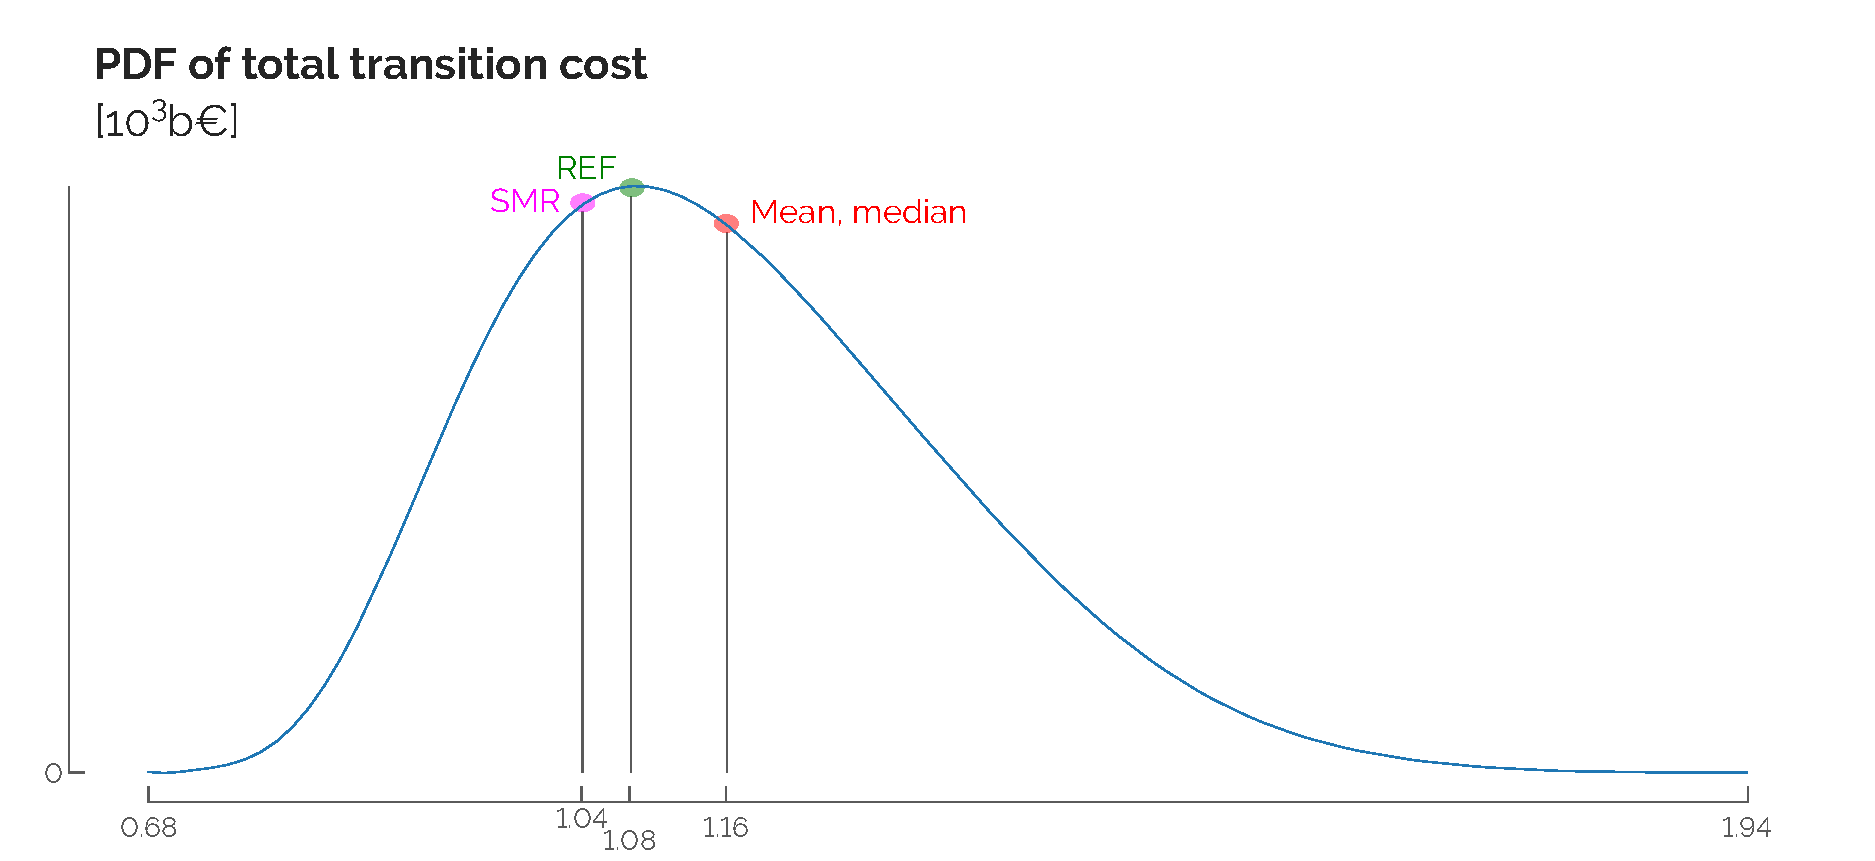
\includegraphics[width=0.6\textwidth]{figures/UQ_PDF_total_transition_cost.pdf}
\caption{\acrfull{PDF} of the total transition cost. The mean, $\mu=1.16\cdot10^3$\,b€, is slightly higher than the median ($P_{50}=1.15\cdot10^3$\,b€) and the nominal cases cost, $1.08\cdot10^3$\,b€ and $1.04\cdot10^3$\,b€ respectively for the REF and SMR cases. Also, with a standard deviation, $\sigma=185$\,b€, a 95\%-confidence interval would be about [0.8; 1.5]$\cdot10^3$\,b€.}
\label{fig:UQ_PDF_total_transition_cost}
\end{figure}

\Cref{tab:UQ_full} gives the ranking and total Sobol index over the total transition cost of each of the 34 parameters listed in \Cref{tab:UC_full}. The first column shows these indicators for the \gls{GSA} applied on the monthly pathway model that has some limitations \cite{limpens2023pathway} but has the main advantage to run much faster. The second column gives the same indicators but for an uncertainty quantification carried out on the hourly pathway model and only using the impacting parameters respecting the good practice rule-of-thumb \cite{Turati2017}\footnote{Parameters are considered as ``impacting'' if their Sobol' index is above the threshold $= 1/d$ (where $d=34$ is the total number of uncertain parameters after the pre-selection phase)}, \ie the top-4 parameters, and some more. Given the similar rankings of the parameters between these two, this comparison shows that the monthly model can be a computationally efficient proxy to quantify the uncertainties of the actual hourly model and point out the key parameters on optimisation-driving objective, the total transition cost. 

Besides the top-4 parameters, rankings are slightly different. However, this does not jeopardize the comparative analysis given the similar Sobol' indices. Given their wide range of uncertainty [-64.3\%; 179.8\%] and their significant role to meet the \ce{CO2}-budget, the cost of purchasing of electrofuels is the first, by far, impacting parameter. Next, comes, naturally, the industrial \gls{EUD}, representing, at the nominal value, 60\% of the total demands by 2050. The top-3 is completed by the variation of the interest rate, directly impacting the annualisation and the salvage values of the assets. Finally, since the current Belgian whole-energy system deeply relies on fossil resources, and would still do in the near future, the cost of purchasing of fossil fuels is part of the impacting parameters. In the contrary, due to the very low annualised, cost, long lifetime leading to a significant salvage value  and a low-emitting fuel, the parameters related to nuclear SMR barely impact the total transition cost.

\begin{table}[htbp]
\caption{Total Sobol' indices of the uncertain parameters over the total transition cost in the monthly and hourly pathway models. The similar rankings (and indices) show the validity of using the faster (even though less accurate) monthly model to assess uncertainties over the hourly model. Abbreviations: \acrfull{EUD}, \acrfull{FC}, \acrfull{HH}, \acrfull{ICE}, \acrfull{LT}, \acrfull{PV}.}
\label{tab:UQ_full}
\centering
\begin{tabular}{l c c| c c}
\toprule
\multirow{2}{*}{\textbf{Parameter}}  & \multicolumn{4}{c}{\textbf{Ranking (Sobol' index)}}\\
 & \multicolumn{2}{c|}{Monthly model} 	& \multicolumn{2}{c}{Hourly model} \\ 	
\midrule
\textbf{Purchase electrofuels} & 1 & (47.4\%) & 1 & (44.4\%) \\
Industry EUD & 2 & (23.5\%) & 2 & (26.4\%)  \\
Interest rate & 3 & (11.0\%) &  3 & (13.2\%)  \\
Purchase fossil fuels  & 4 & (6.9\%) & 4 & (6.9\%)   \\
\midrule
Variable opex of technologies & 5 & (2.9\%) & 6 & (3.0\%) \\
Purchase biofuels & 6 & (2.6\%) & 5 & (3.0\%) \\
Hourly load factor PV & 7 & (1.9\%) & 9 & (1.3\%) \\
Capex electric motor & 8 & (1.9\%) & 7 & (2.5\%) \\
Hourly load factor wind turbines & 9 & (1.3\%) & 8 & (1.4\%) \\
Max capacity PV & 10 & (1.1\%) & 14 & (0.5\%) \\
\textbf{Potential capacity nuclear SMR} & 11 & (0.9\%) & 11 & (1.0\%) \\
Available local biomass & 12 & (0.8\%) & 12 & (0.7\%) \\
Capex car & 13 & (0.7\%) & 10 & (1.2\%) \\
Passenger mobility EUD & 14 & (0.7\%) & 13 & (0.7\%) \\
\midrule
Modal share change LT-heat & 15 & (0.5\%) & \multicolumn{2}{c}{-} \\
Households EUD & 16 & (0.5\%) & \multicolumn{2}{c}{-} \\
Services EUD & 17 & (0.4\%) & \multicolumn{2}{c}{-} \\
Max capacity onshore wind & 18 & (0.3\%) & \multicolumn{2}{c}{-} \\
Max share of public transport & 19 & (0.3\%) & \multicolumn{2}{c}{-} \\
Capex PV & 20 & (0.2\%) & \multicolumn{2}{c}{-} \\
Max capacity offshore wind & 21 & (0.2\%) & \multicolumn{2}{c}{-} \\
Efficiency electric motor & 22 & (0.1\%) & \multicolumn{2}{c}{-} \\
Capex fuel cell engine & 23 & (0.1\%) & \multicolumn{2}{c}{-} \\
Capex ICE & 24 & (0.1\%) & \multicolumn{2}{c}{-} \\
Efficiency fuel cell engine & 25 & ($<$0.1\%) & \multicolumn{2}{c}{-} \\
Modal share change freight mobility & 26 & ($<$0.1\%) & \multicolumn{2}{c}{-} \\
Modal share change passenger mobility & 27 & ($<$0.1\%) & \multicolumn{2}{c}{-} \\
Capex efficiency measures & 28 & ($<$0.1\%) & \multicolumn{2}{c}{-} \\
Capex bus & 29 & ($<$0.1\%) & \multicolumn{2}{c}{-} \\
Capex grid reinforcement & 30 & ($<$0.1\%) & \multicolumn{2}{c}{-} \\
Capex power grid & 31 & ($<$0.1\%) & \multicolumn{2}{c}{-} \\
\textbf{Capex nuclear SMR} & 32 & ($<$0.1\%) & \multicolumn{2}{c}{-} \\
Available electricity import & 33 & ($<$0.1\%) & \multicolumn{2}{c}{-} \\
Purchase electricity & 34 & ($<$0.1\%) & \multicolumn{2}{c}{-} \\
\bottomrule							

\end{tabular}
\end{table}

% \begin{table}[htbp]
% \caption{Total Sobol' indices of the uncertain parameters over the total transition cost in the monthly and hourly pathway models. The similar rankings (and indices) show the validity of using the faster (even though less accurate) monthly model to assess uncertainties over the hourly model. Abbreviations: \acrfull{EUD}, \acrfull{FC}, \acrfull{HH}, \acrfull{ICE}, \acrfull{LT}, \acrfull{PV}.}
% \label{tab:UQ_full}
% \centering
% \begin{tabular}{l c c| c c}
% \toprule
% \multirow{2}{*}{\textbf{Parameter}}  & \multicolumn{4}{c}{\textbf{Ranking (Sobol' index)}}\\
%  & \multicolumn{2}{c|}{Hourly model} 	& \multicolumn{2}{c}{Model model} \\ 	
% \midrule
% Purchase electrofuels & 1 & (44.4\%) & 1 & (47.4\%) \\
% Industry EUD & 2 & (26.4\%) & 2 & (23.5\%)  \\
% Interest rate & 3 & (13.2\%) &  3 & (11.0\%)  \\
% Purchase fossil fuels & 4 & (6.9\%)  & 4 & (6.9\%)  \\
% \midrule
% Purchase biofuels & 5 & (3.0\%) & 6 & (2.6\%)  \\
% Variable opex of technologies & 6 & (3.0\%) & 5 & (2.9\%) \\
% Capex electric motor & 7 & (2.5\%) & 8 & (1.9\%)  \\
% Hourly load factor wind turbines & 8 & (1.4\%) & 9 & (1.3\%) \\ 
% Hourly load factor PV & 9 & (1.3\%) & 7 & (1.9\%)  \\
% Capex car & 10 & (1.2\%) & 13 & (0.7\%) \\
% \textbf{Potential capacity nuclear SMR} & 11 & (1.0\%) & 11 & (0.9\%)  \\
% Available local biomass & 12 & (0.7\%)  & 12 & (0.8\%) \\
% Passenger mobility EUD & 13 & (0.7\%) & 14 & (0.7\%) \\
% Max capacity PV & 14 & (0.5\%) & 10 & (1.1\%)  \\
% \midrule
% Modal share change LT-heat & \multicolumn{2}{c}{-} & 15 & (0.5\%)  \\
% Households EUD & \multicolumn{2}{c}{-} & 16 & (0.5\%) \\
% Services EUD & \multicolumn{2}{c}{-} & 17 & (0.4\%) \\
% Max capacity onshore wind & \multicolumn{2}{c}{-} & 18 & (0.3\%) \\
% Max share of public transport & \multicolumn{2}{c}{-} & 19 & (0.3\%) \\
% Capex PV & \multicolumn{2}{c}{-} & 20 & (0.2\%) \\
% Max capacity offshore wind & \multicolumn{2}{c}{-} & 21 & (0.2\%)\\
% Efficiency electric motor & \multicolumn{2}{c}{-}  & 22 & (0.1\%) \\
% Capex fuel cell engine & \multicolumn{2}{c}{-}  & 23 & (0.1\%) \\
% Capex ICE & \multicolumn{2}{c}{-} & 24 & (0.1\%)\\
% Efficiency fuel cell engine & \multicolumn{2}{c}{-}  & 25 & ($<$0.1\%) \\
% Modal share change freight mobility & \multicolumn{2}{c}{-}  & 26 & ($<$0.1\%) \\
% Modal share change passenger mobility & \multicolumn{2}{c}{-}  & 27 & ($<$0.1\%)\\
% Capex efficiency measures & \multicolumn{2}{c}{-}  & 28 & ($<$0.1\%)\\
% Capex bus & \multicolumn{2}{c}{-}  & 29 & ($<$0.1\%)\\
% Capex grid reinforcement & \multicolumn{2}{c}{-} & 30 & ($<$0.1\%) \\
% Capex power grid & \multicolumn{2}{c}{-} & 31 & ($<$0.1\%)\\
% \textbf{Capex nuclear SMR} & \multicolumn{2}{c}{-} & 32 & ($<$0.1\%) \\
% Available electricity import & \multicolumn{2}{c}{-}  & 33 & ($<$0.1\%) \\
% Purchase electricity  & \multicolumn{2}{c}{-} & 34 & ($<$0.1\%)\\
% \bottomrule							

% \end{tabular}
% \end{table}

\subsection{Imported renewable electrofuels}
\label{app:UQ_electrofuels}
\begin{table}[htbp]
\caption{Comparison of the quantities of imported renewable electrofuels, in TWh, between the REF case, the SMR case and the statistical features from the \gls{GSA} (\ie Q1, median and Q3). 2020 is not in the table as, per assumption, no renewable electrofuel is imported for this year. For the sake of clarity, zeros are replaced by ``-''.}
\label{tab:uq_ref_smr_med}
\begin{minipage}{\linewidth}
\centering
\begin{tabular}{l l | c c c c}
\toprule
\textbf{Year} & \textbf{Case} & \textbf{e-methane} & \textbf{e-hydrogen} & \textbf{e-ammonia} & \textbf{e-methanol}\\	
\toprule							
\multirow{5}{*}{2025}
 & REF & - & - & 10 & 52\\
 & SMR & - & -  & 10 & 29\\
 \cmidrule{2 - 6}
 & Q1 & - & - & 9 & 2\\
 & Median & - & - & 10 & 46\\
 & Q3 & - & - & 11 & 55\\
\toprule
\multirow{5}{*}{2030}
 & REF & - & 1 & 10 & 52\\
 & SMR & - & 1 & 10 & 52\\
 \cmidrule{2 - 6}
 & Q1 & - & - & 9 & 43\\
 & Median & - & - & 10 & 51\\
 & Q3 & - & 1 & 12 & 57\\
\toprule
\multirow{5}{*}{2035}
 & REF & - & 17 & 10 & 53\\
 & SMR & - & 17 & 10 & 53\\
 \cmidrule{2 - 6}
 & Q1 & - & - & 9 & 44\\
 & Median & - & 4 & 11 & 52\\
 & Q3 & - & 16 & 32 & 58\\
\toprule
\multirow{5}{*}{2040}
 & REF & - & 16 & 23 & 54\\
 & SMR & - & 16 & 10 & 54\\
 \cmidrule{2 - 6}
 & Q1 & - & - & 12 & 43\\
 & Median & - & 12 & 36 & 53\\
 & Q3 & 10 & 16 & 68 & 60\\
\toprule
\multirow{5}{*}{2045}
 & REF & 40 & 16 & 42 & 54\\
 & SMR & - & 16 & 11 & 54\\
 \cmidrule{2 - 6}
 & Q1 & - & - & 24 & 43\\
 & Median & - & 13 & 49 & 52\\
 & Q3 & 44 & 17 & 77 & 60\\
\toprule
\multirow{5}{*}{2050}
 & REF & 39 & 16 & 44 & 55\\
 & SMR & 7 & 16 & 11 & 55\\
 \cmidrule{2 - 6}
 & Q1 & - & - & 20 & 44\\
 & Median & 19 & 14 & 44 & 53\\
 & Q3 & 51 & 17 & 72 & 61\\
\bottomrule							
\end{tabular}
\end{minipage}
\end{table}

\begin{figure}[!htbp]
\centering
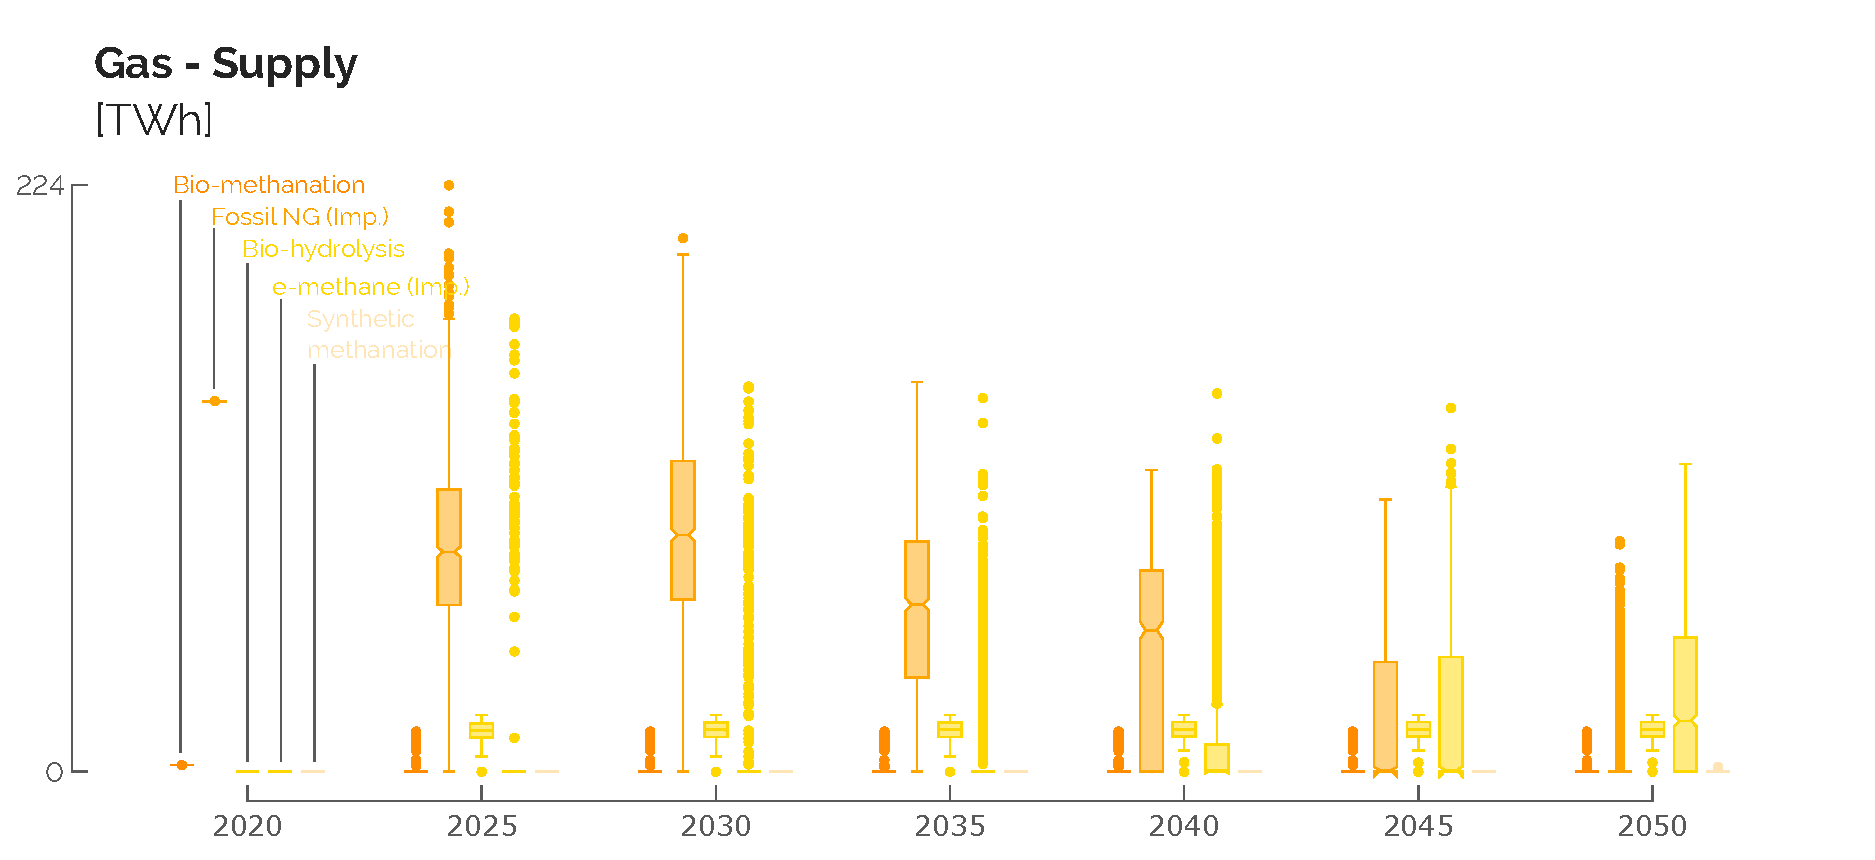
\includegraphics[width=0.49\textwidth]{figures/UQ_Gas_Prod.pdf}
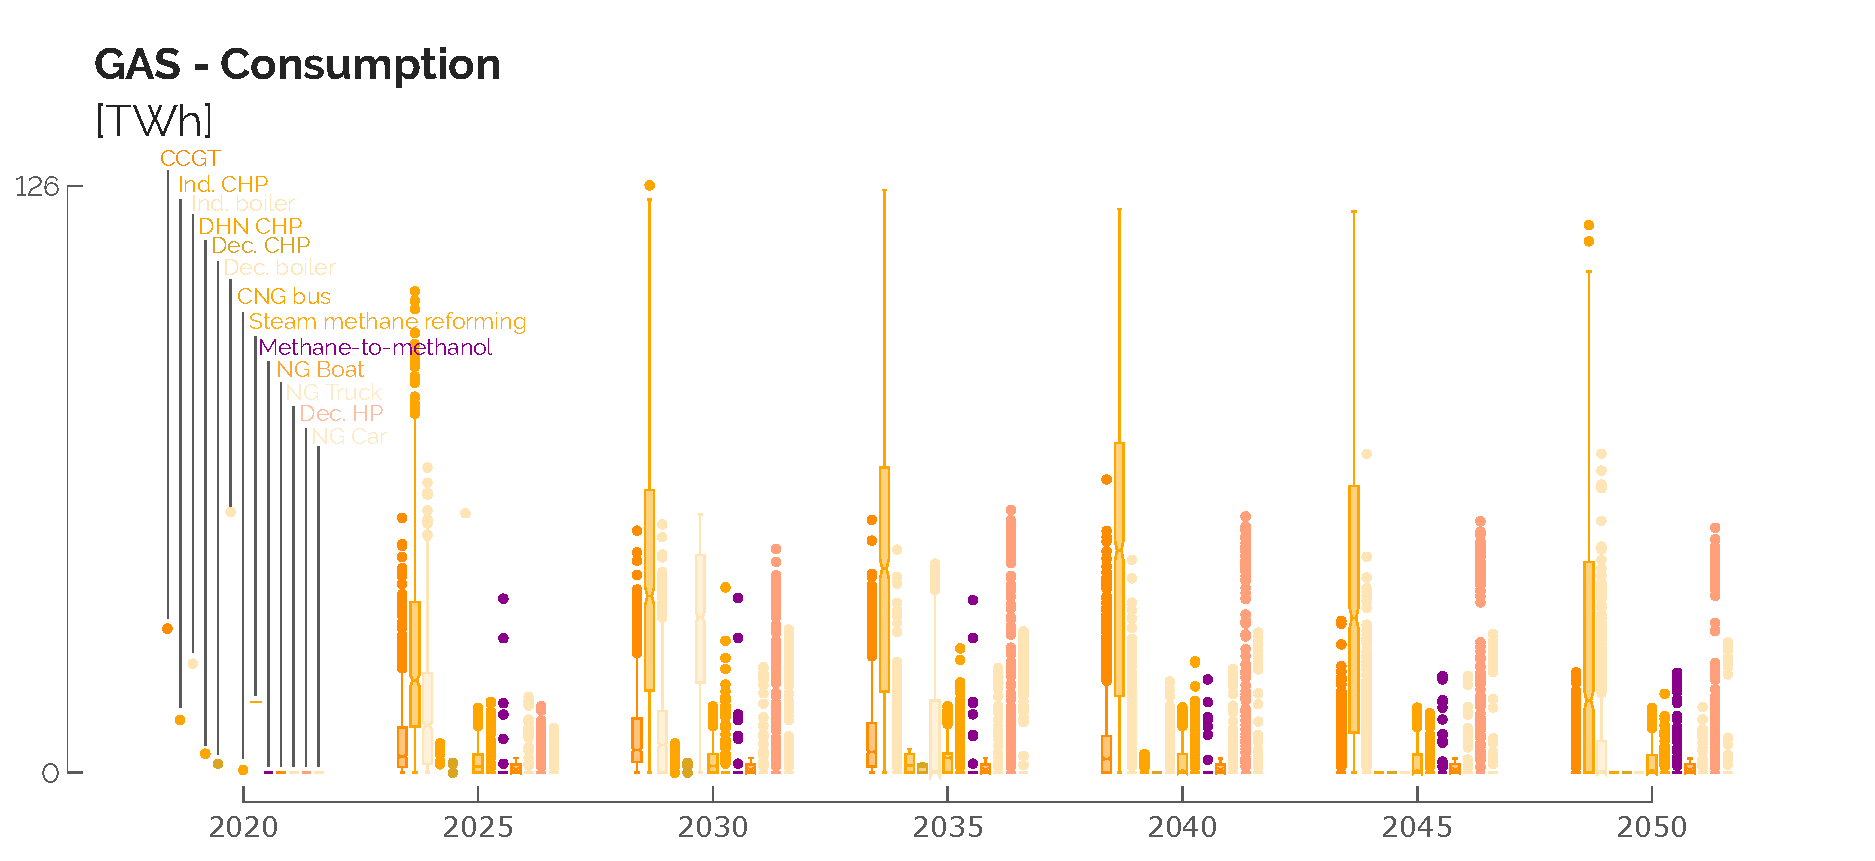
\includegraphics[width=0.49\textwidth]{figures/UQ_Gas_Cons.pdf}
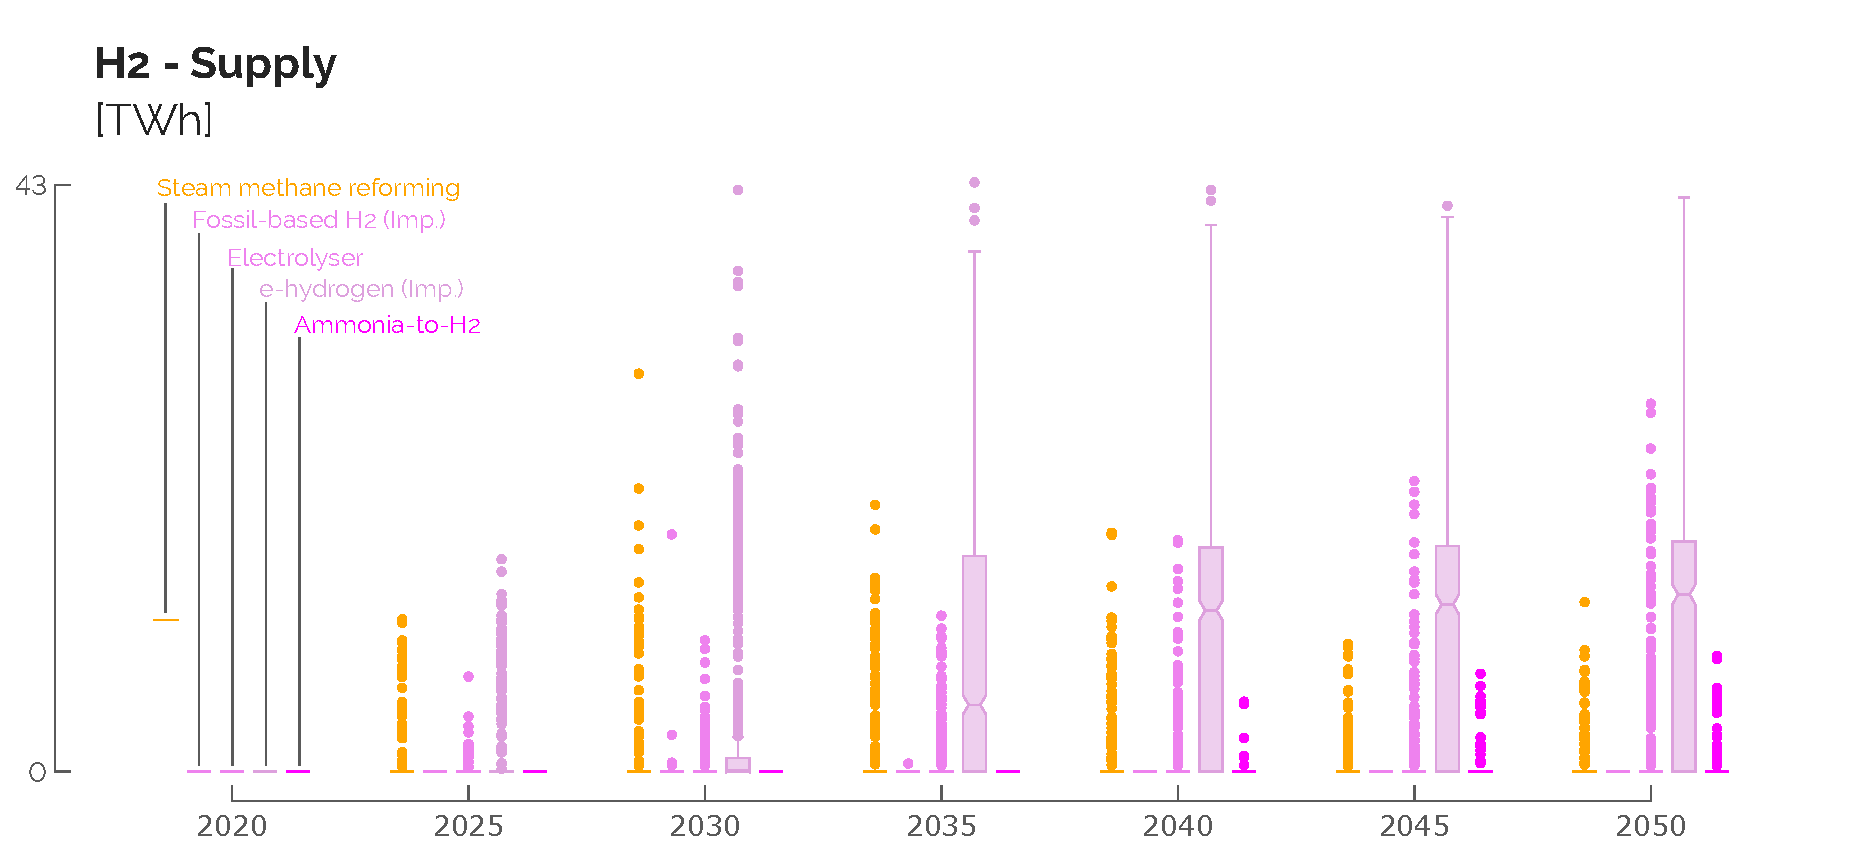
\includegraphics[width=0.49\textwidth]{figures/UQ_H2_Prod.pdf}
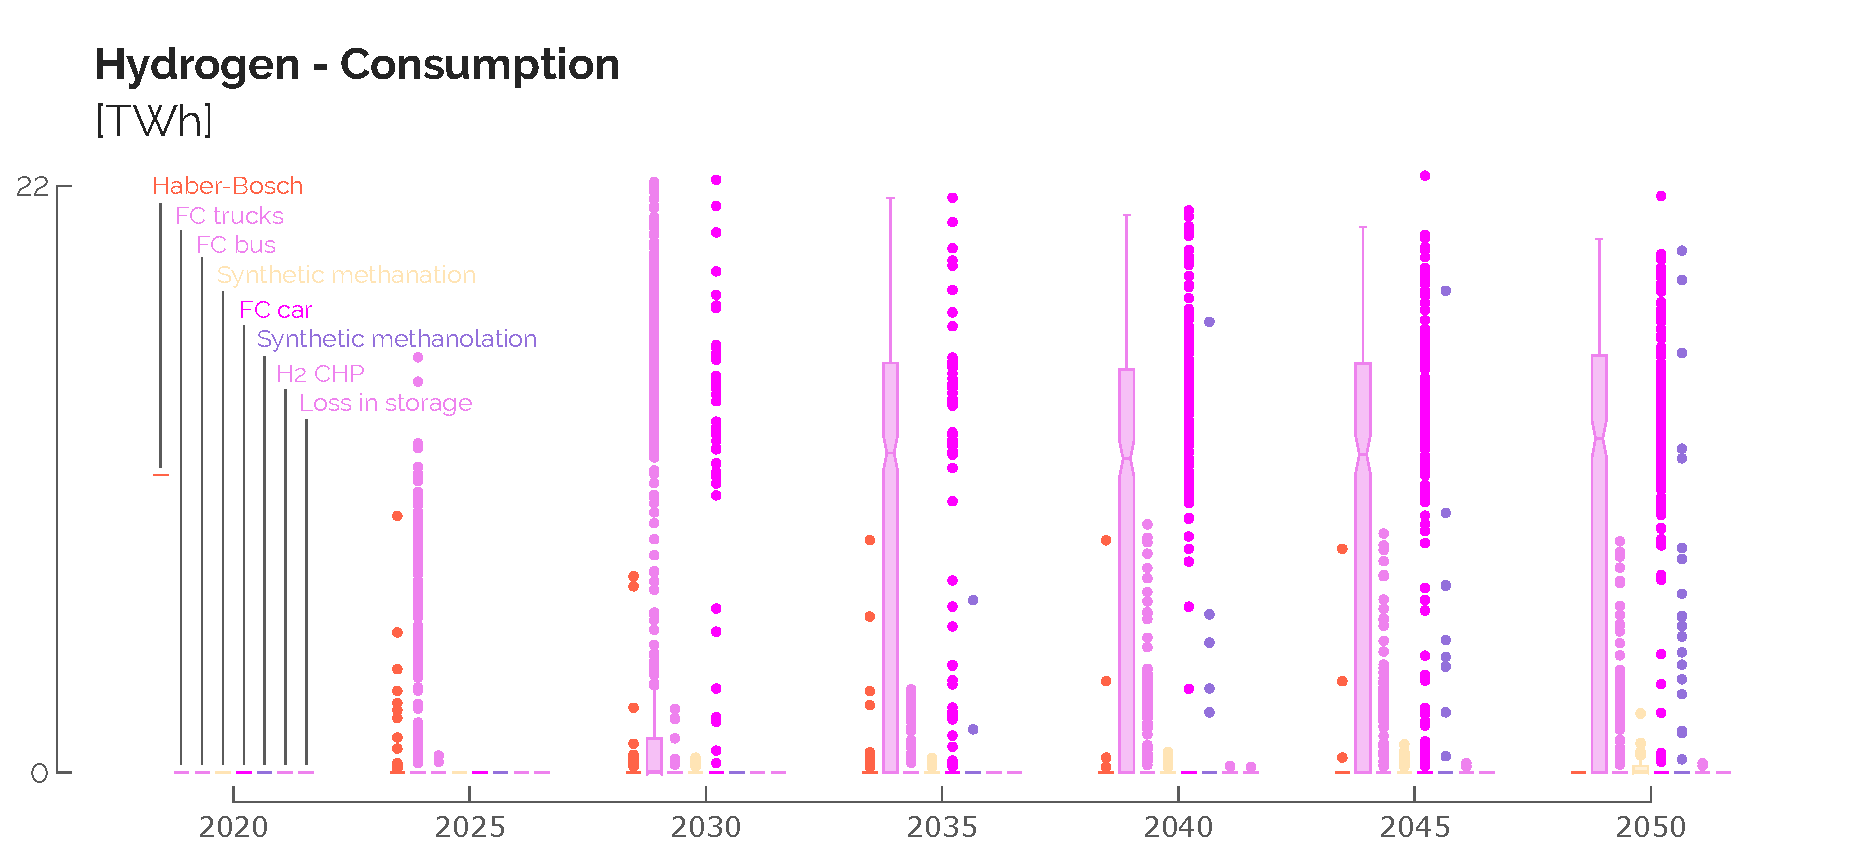
\includegraphics[width=0.49\textwidth]{figures/UQ_H2_Cons.pdf}
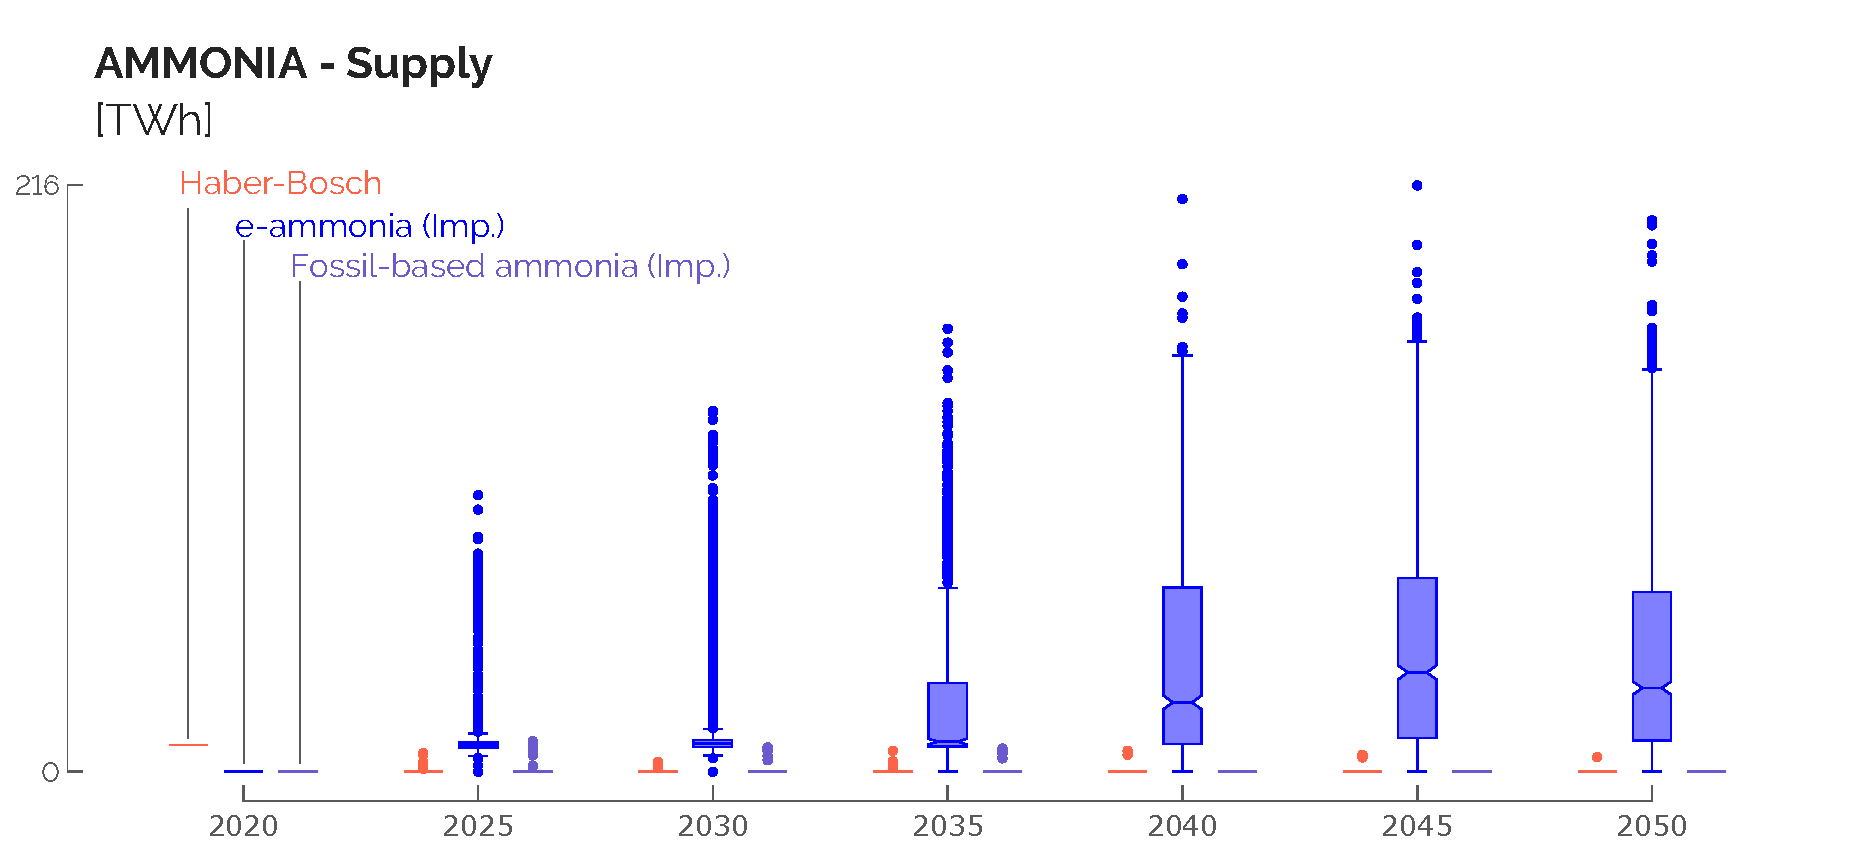
\includegraphics[width=0.49\textwidth]{figures/UQ_Ammonia_Prod.pdf}
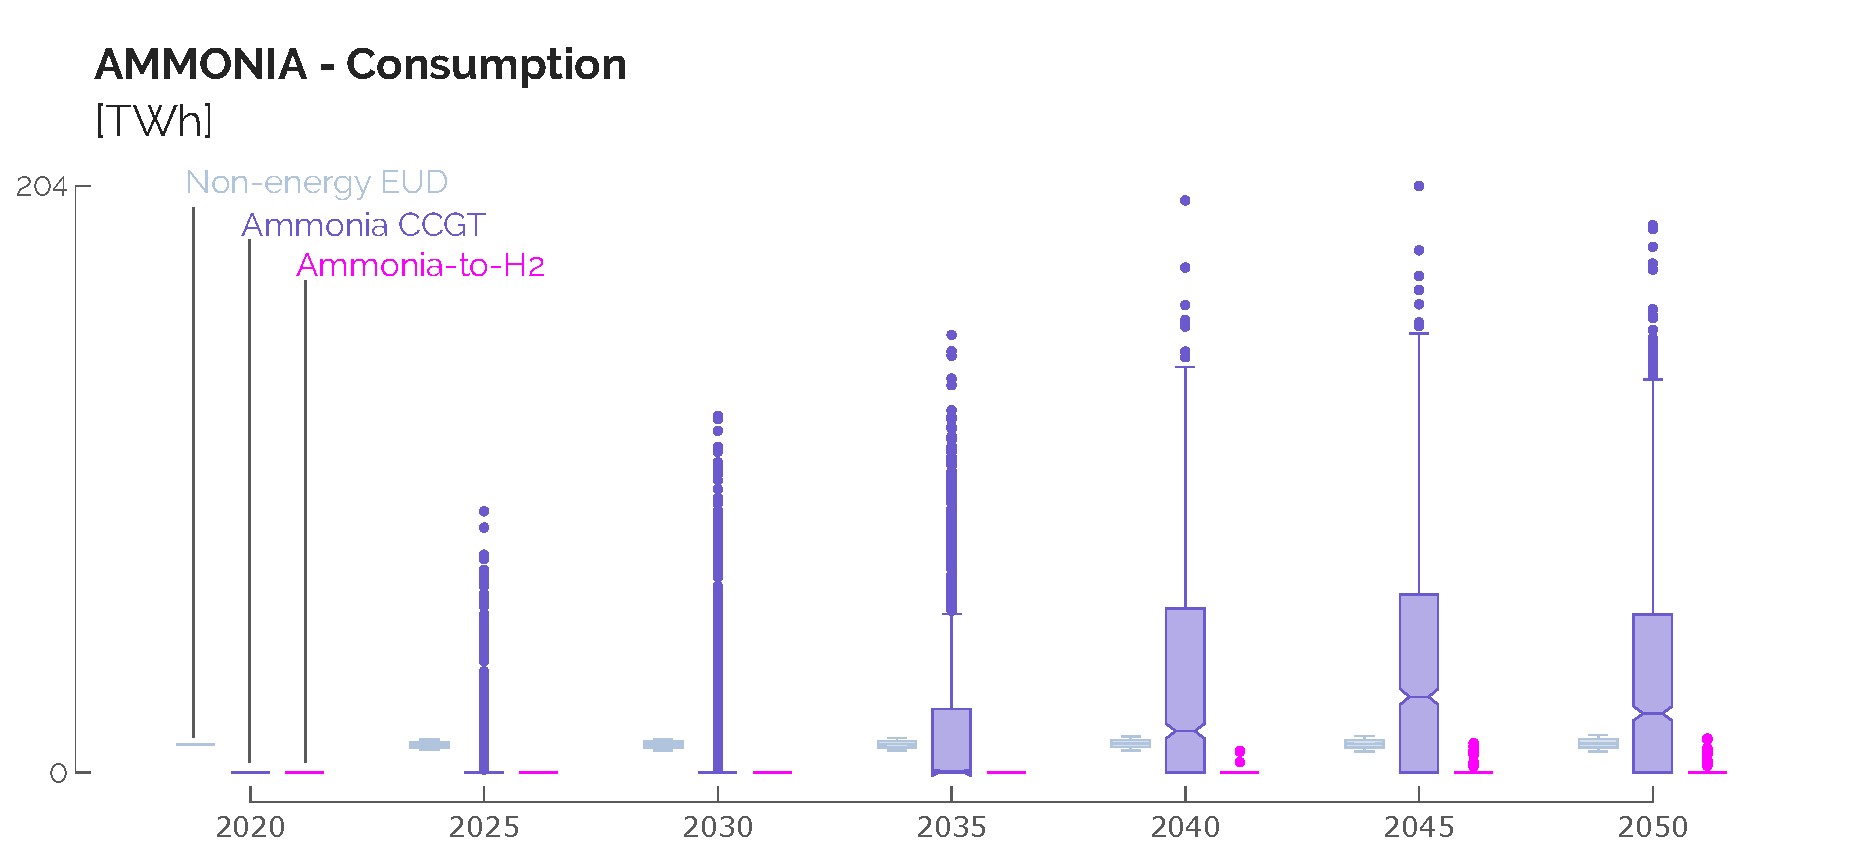
\includegraphics[width=0.49\textwidth]{figures/UQ_Ammonia_Cons.pdf}
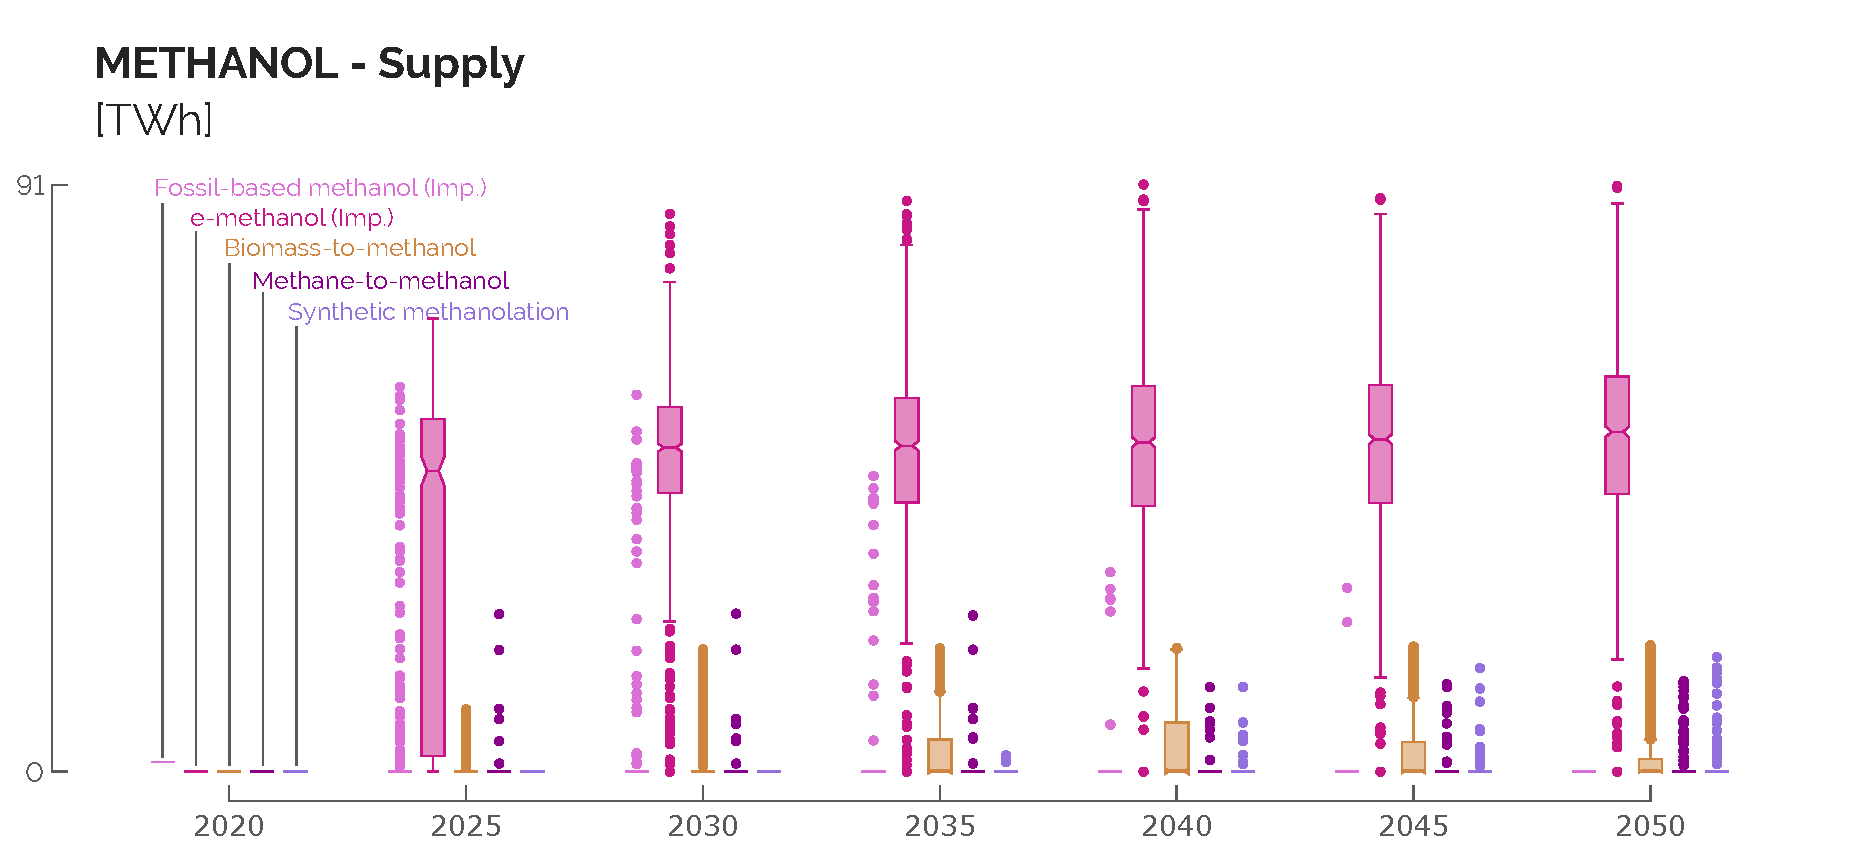
\includegraphics[width=0.49\textwidth]{figures/UQ_Methanol_Prod.pdf}
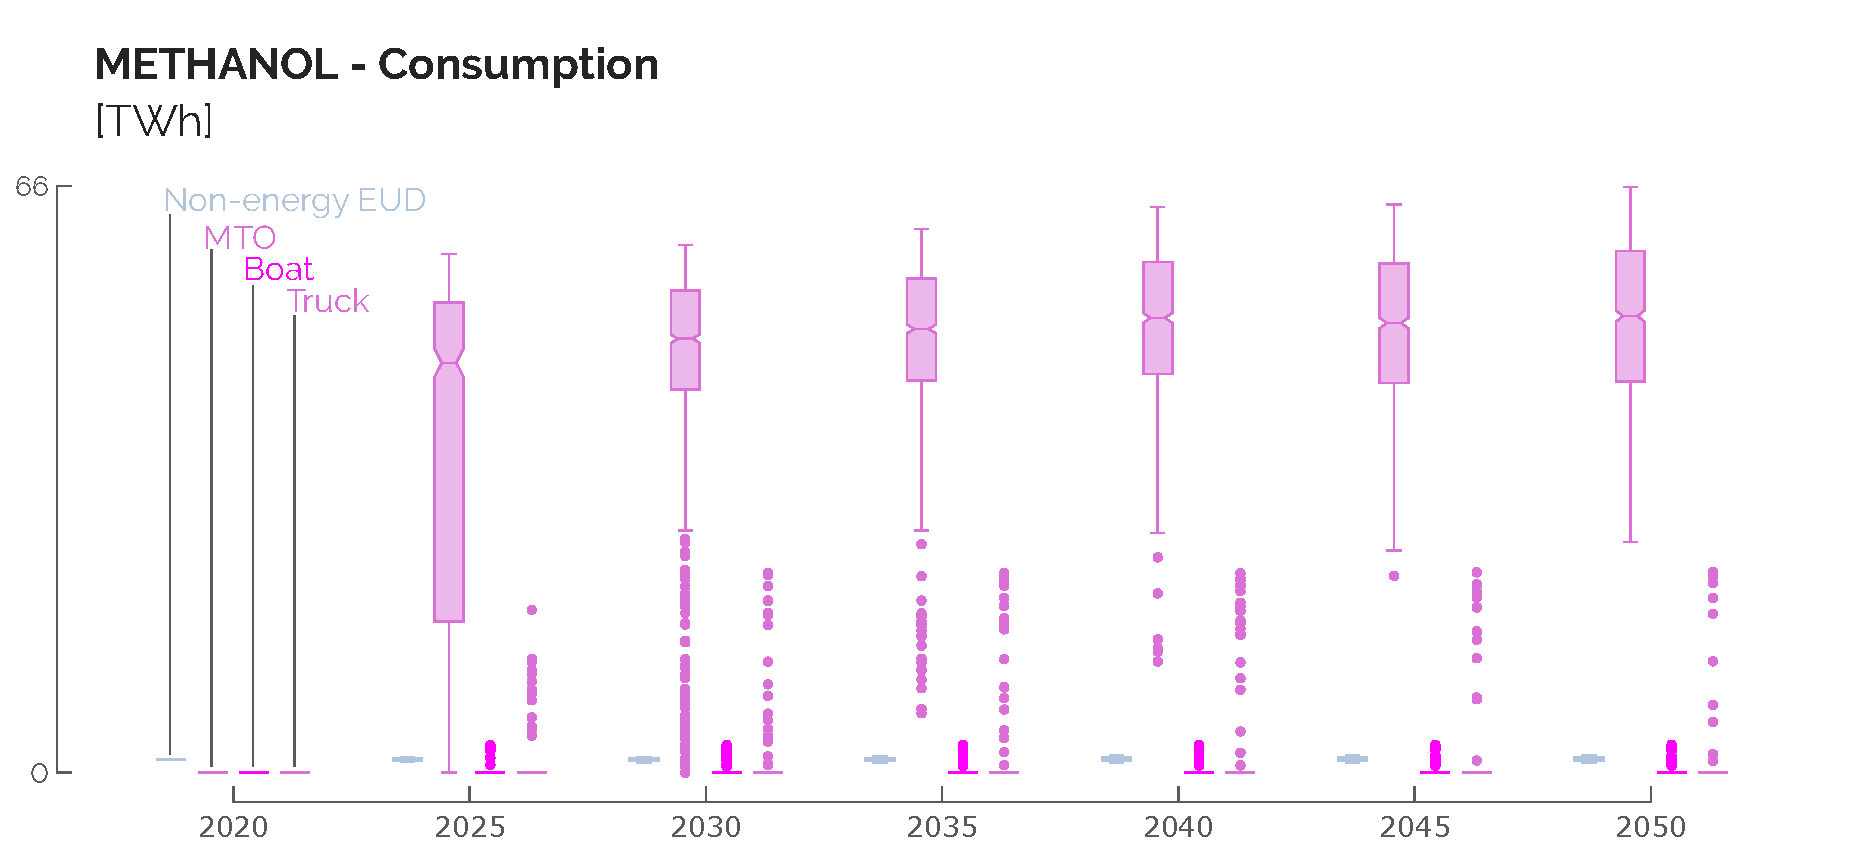
\includegraphics[width=0.49\textwidth]{figures/UQ_Methanol_Cons.pdf}
\caption{Distribution of the different streams of supply and consumption of gas, hydrogen, ammonia and methanol from the \acrfull{GSA}. Abbreviations: \acrfull{CCGT}, \acrfull{CHP}, \acrfull{CNG}, decentralised (DEC), \acrfull{DHN}, \acrfull{EUD}, \acrfull{FC}, \acrfull{HP}, imported (Imp.), industrial (Ind.), \acrfull{MTO}}
\label{fig:results_uq_prod_cons}
\end{figure}




\end{appendices}


\newpage

\section*{Acknowledgement}
Authors acknowledge the support of the Energy Transition Fund of Belgium.

%\section{References}
% If not using biblatex
% To set the bibliography style
%\bibliographystyle{unsrt} 
%\bibliography{bibliography/biblio}{}
% If using biblatex
\printbibliography[heading=bibintoc]
\end{document}
%%%%%%%%% End of the Report %%%%%%%%%